\documentclass[12pt]{report}
\usepackage{multirow}
\usepackage{rotating}
\usepackage{hhline}
\usepackage[]{graphicx}
\usepackage[left=1.5in, right=1in,top=1in,bottom=1in,headheight=6pt, a4paper]{geometry}
\usepackage{titling}
\usepackage{booktabs}
\usepackage[numbers]{natbib}
% \usepackage{biblatex}
%\usepackage{times}
\usepackage{microtype}
\usepackage[utf8x]{inputenc}
\usepackage{xcolor}
\usepackage{datetime2}
\usepackage{tabto}
\usepackage{enumitem}
\usepackage[font=normalsize,tableposition=top]{caption}
\usepackage{etoolbox}\usepackage{setspace}
\usepackage[explicit]{}
\usepackage{algpseudocode, algorithm}
\usepackage{amsmath}
\usepackage{amsfonts}
\usepackage{amssymb}
\usepackage{hyperref}
\usepackage{pgfgantt}
\usepackage{adjustbox}
\usepackage{multicol}
\usepackage{mathptmx}
\usepackage{titlesec}
\usepackage{setspace}
\usepackage{import}
\usepackage{enumitem}
\usepackage{bm}
\usepackage{amsmath, amsfonts}
\usepackage{pdflscape}
\usepackage{everypage-1x}
\usepackage{wrapfig}
\usepackage{scrextend}
\usepackage{etoolbox}
\usepackage{appendix}
\usepackage{multicol}
\usepackage{svg}


\renewcommand\appendixtocname{APPENDIX}
\renewcommand\appendixpagename{APPENDIX}
\renewcommand{\bibname}{REFERENCES}

%\usetikzlibrary{positioning}
% \ganttset{group/.append style={orange},
% milestone/.append style={red},
% progress label node anchor/.append style={text=red}}

\linespread{1.3}
\setlength{\parskip}{6pt}
\setlength{\parindent}{0em}


%--------------------



%------ SET DOCUMENT GEOMETRY ------%
\usepackage{geometry}
\geometry{a4paper, left=1.5in, top=1in, bottom=1in, right=1in}


%------ FORMAT CHAPTER, SECTION, AND SUBSECTION TITLE ------%

 \titleformat{\chapter}
 {\normalfont\centering\fontsize{14}{15}\bfseries}
 {\MakeUppercase{\chaptertitlename} \thechapter}
 {0.5em}
 {\MakeUppercase}

  % \titleformat{\chapter}{
  % \normalfont\fontsize{12}{15}\bfseries
  % }{\thechapter}{1em}{}

  \titleformat{\section}{
  \normalfont\fontsize{12}{15}\bfseries
  }{\thesection}{1em}{}

  \titleformat{\subsection}{
  \normalfont\fontsize{12}{15}\bfseries
  }{\thesubsection}{1em}{}

  % \titlespacing{\chapter}{0pt}{-0.5in}{-0.5em}
  % \titlespacing{\chapter}{0pt}{180pt}{1em}
  \titlespacing{\chapter}{0pt}{-0.5in}{1em}
  \titlespacing{\section}{0pt}{0pt}{-1em}
  % \titlespacing{\section}{0pt}{0pt}{1pt}

  \titlespacing{\subsection}{0pt}{0pt}{-1em}
  % \titlespacing{\subsection}{0pt}{0pt}{2pt}


%------ SET SPACING AND INDENTS ------%
\renewcommand{\baselinestretch}{1.5} 
\setlength{\parindent}{0pt}
\setlength{\parskip}{12pt}


%------ SETUP LINKS ------%
\usepackage{hyperref}
\hypersetup{
    colorlinks,
    citecolor=black,
    filecolor=black,
    linkcolor=black,
    urlcolor=black
}


%------ FORMAT TABLE OF CONTENTS ------%
\usepackage{tocloft}


\cftsetindents{section}{1.4em}{1.75em}
\cftsetindents{subsection}{3.2em}{2.6em}
\setlength{\cftbeforetoctitleskip}{-2.5em}
\setlength{\cftbeforechapskip}{0.25em}

\renewcommand{\cftchapleader}{\dotfill}

\renewcommand{\cftdotsep}{1.5}
\renewcommand{\cftsecfont}{\normalfont}
\renewcommand{\cftsecpagefont}{\normalfont}

\setlength{\cftbeforeloftitleskip}{-2.5em}
\setlength{\cftbeforelottitleskip}{-2.5em}

\setlength{\cftfigindent}{0pt}
\setlength{\cfttabindent}{0pt}

\renewcommand{\cftfigfont}{Figure }
\renewcommand{\cfttabfont}{Table }


%------ FORMAT TABLE CAPTIONS ------%
\usepackage{caption} 
\captionsetup[table]{skip=10pt}



\newcommand{\Lpagenumber}{\ifdim\textwidth=\linewidth\else\bgroup
  \dimendef\margin=0 %use \margin instead of \dimen0
  \ifodd\value{page}\margin=\oddsidemargin
  \else\margin=\evensidemargin
  \fi
  \raisebox{\dimexpr -\topmargin-\headheight-\headsep-0.5\linewidth}[0pt][0pt]{%
    \rlap{\hspace{\dimexpr \margin+\textheight+\footskip}%
    \llap{\rotatebox{90}{\thepage}}}}%
\egroup\fi}
\AddEverypageHook{\Lpagenumber}%


\newcommand{\theinstitute}{Institute of Engineering}
\newcommand{\thecampus}{Lalitpur Engineering College}
\newcommand{\thedepartment}{Department of Computer Engineering}
\newcommand{\thedepartmentAddress}{Kathmandu, Nepal}
\newcommand{\thedepartmentFullAddress}{Chakupat, Lalitpur, Nepal}
\newcommand{\theprogramcoordinator}{Er. Bisikha Subedi}
\newcommand{\theHOD}{Er. Praches Acharya}
\newcommand{\thesupervisor}{Er. Praches Acharya}




\title{\MakeUppercase{Parichaya}: A Digital Identity Ecosystem based on Hyperledger Fabric}
\author{Asim Nepal [LEC075BCT003]
\\Dikshya Kunwar [LEC075BCT005]
\\Kushal Koirala [LEC075BCT020]
\\Nischal Shakya [LEC075BCT010]} 
\date{March, 2023}



\begin{document}
{
	\thispagestyle{empty}
	\centering
	% \normalsize
	  % \begin{large}
   \fontsize{14pt}{14pt}\selectfont
        	\textbf{\MakeUppercase{Tribhuvan University}}\\
        	\textbf{\MakeUppercase{INSTITUTE OF ENGINEERING}}\\[0.5cm]
        	% \includegraphics[width=1.3in]{images/TUlogo.png}\\[0.5cm]
        	% 
\includegraphics[width=3in]{images/LECLogo.png}\\[0.3cm]
        	
\includegraphics[width=3in]{images/LECLogo.jpg}\\[0.3cm]
        	\textbf{\MakeUppercase{Lalitpur Engineering College}}\\
    	\textbf{Kholcha Pokhari, Chakupat, Lalitpur}\\[1.4cm]
        % \end{large}
    	
	  % \begin{normalsize}
    	\textbf{\MakeUppercase{A final year project report on}}\\
        % \end{normalsize}
    	\textbf{"\MakeUppercase{Parichaya}: A Digital Identity Ecosystem based on \\ Hyperledger Fabric"}\\
    	\textbf{[CT 755]}\\[2cm]
    	
	  % \begin{normalsize}
    	\textbf{\MakeUppercase{Submitted To:}}\\
    	{Department of Computer Engineering}\\[1.2cm]
    	\textbf{\MakeUppercase{Submitted By:}}\\
            {
        	{{Asim Nepal (LEC075BCT003)}}\\
        	{{Dikshya Kunwar (LEC075BCT005)}}\\
        	{{Kushal Koirala (LEC075BCT020)}}\\
        	{{Nischal Shakya (LEC075BCT010)}}\\[1.2cm]
        	% {\MakeUppercase{Asim Nepal (LEC075BCT003)}}\\
        	% {\MakeUppercase{Dikshya Kunwar (LEC075BCT005)}}\\
        	% {\MakeUppercase{Kushal Koirala (LEC075BCT020)}}\\
        	% {\MakeUppercase{Nischal Shakya (LEC075BCT010)}}\\[1.2cm]
            }	
     \textbf{\MakeUppercase{Lalitpur, Nepal}}\\
    	\textbf{2023}\\
        % \end{large}
}


{
    \thispagestyle{empty}
    \centering

   \fontsize{14pt}{14pt}\selectfont
        {A Final Year Project Report}\\ 
        {On}\\[1.5cm]

        
         % \begin{LARGE}
            \textbf{"\MakeUppercase{Parichaya}: A Digital Identity Ecosystem based on \\ Hyperledger Fabric"}\\
            \textbf{[CT 755]}\\[2cm]
        % \end{LARGE}
    {Submitted as a partial fulfillment of requirement of the curriculum of Bachelor of Computer Engineering under TU}\\[3cm]
    \textbf{\MakeUppercase{Submitted By:}}\\
    {Asim Nepal}\\
    {Dikshya Kunwar}\\
    {Kushal Koirala}\\
    {Nischal Shakya}\\[2.5cm]
    % \MakeUppercase{Asim Nepal}\\
    % \MakeUppercase{Dikshya Kunwar}\\
    % \MakeUppercase{Kushal Koirala}\\
    % \MakeUppercase{Nischal Shakya}\\[2.5cm]
    
    \textbf{\MakeUppercase{Under Supervision Of:}}\\
    {Er. Praches Acharya}\\[2.5cm]
    % \MakeUppercase{Er. Praches Acharya}\\[2.5cm]
    
        \textbf{April, 2023}\\
% \end{large}
}

\pagenumbering{Roman}
\titlespacing{\chapter}{0pt}{-0.5in}{1em}
\chapter*{\vspace{0.4cm}\centerline{COPYRIGHT \textcopyright}}
\addcontentsline{toc}{chapter}{COPYRIGHT}
\vspace{-1cm}
The authors have agreed that the library, \thedepartment, \theinstitute, \thecampus, may make this project
work freely available for inspection. Moreover the author has agreed that the
permission for extensive copying of this project work for scholarly purpose may be
granted by the professor(s), who supervised the project work recorded herein or, in
their absence, by the Head of the Department, wherein this project work was done. It
is understood that the recognition will be given to the author of this project work and
to the \thedepartment, \theinstitute, \thecampus \ in any use of the material of this project work. Copying of publication or other use of
this project work for financial gain without approval of the \thedepartment, \theinstitute, \thecampus \ and author’s
written permission is prohibited.

Request for permission to copy or to make any use of the material in this project in
whole or part should be addressed to:

\vspace{1cm}

Head\\
\thedepartment\\
\theinstitute, \thecampus\\
\thedepartmentFullAddress



\chapter*{\vspace{0.4cm}\centerline{DECLARATION}}
\addcontentsline{toc}{chapter}{DECLARATION}
\vspace{-1cm}
We declare that the work hereby submitted for Bachelor in Computer Engineering (BCT) at the \theinstitute, \thecampus \ entitled "\textbf{\thetitle}" is our own work and has not been previously submitted by
us at any university for any academic award.
We authorize the \theinstitute, \thecampus \ to lend this project work
to other institutions or individuals for the purpose of scholarly research.

\vspace{1cm}

% {Asim Nepal (LEC075BCT003)} \hspace{0.5em}\rule{0.4\textwidth}{0.4pt}\\[1em]
% {Dikshya Kunwar (LEC075BCT005)}  \hspace{0.5em}\rule{0.4\textwidth}{0.4pt}\\[1em]
% {Kushal Koirala (LEC075BCT020)} \hspace{0.5em}\rule{0.4\textwidth}{0.4pt}\\[1em]
% {Nischal Shakya (LEC075BCT010)} \hspace{0.5em}\rule{0.4\textwidth}{0.4pt}\\[1em]
% \textbf{Date:} March, 2023
{Asim Nepal (LEC075BCT003)}\\
{Dikshya Kunwar (LEC075BCT005)}\\
{Kushal Koirala (LEC075BCT020)}\\
{Nischal Shakya (LEC075BCT010)}\\[1em]
\textbf{Date:} April, 2023


% \newgeometry{left=1.5in, top=2.5in, bottom=1in, right=1in}
% \chapter*{\centerline{RECOMMENDATION}}
\chapter*{\vspace{0.4cm}\centerline{CERTIFICATE OF APPROVAL}}
\addcontentsline{toc}{chapter}{CERTIFICATE OF APPROVAL}
\vspace{-1cm}
The undersigned certify that they have read and recommended to the \textbf{\thedepartment, \thecampus} for acceptance, a project work entitled “\textbf{\thetitle}”, submitted by \textbf{Asim Nepal, Dikshya Kunwar, Kushal Koirala and Nischal Shakya} in partial fulfillment of the requirement
for the award of the degree of “\textbf{Bachelor in Computer Engineering}”.
\vspace{1.4cm}
\begin{multicols}{2}
\rule{0.4\textwidth}{0.4pt}\\
\textbf{Project Supervisor}\\
\thesupervisor\\
\thedepartment\\ 
\thecampus\\
\vfill
\columnbreak
\rule{0.4\textwidth}{0.4pt}\\
\textbf{External Examiner}\\
{Prof. Dr. Subarna Shakya}\\
{Institute of Engineering}\\
{Pulchowk Campus}
\end{multicols}
\vspace{0.4cm}
\begin{multicols}{2}
\rule{0.4\textwidth}{0.4pt}\\
\textbf{Project Co-ordinator}\\
\theprogramcoordinator \\
\thedepartment\\ 
\thecampus\\
\columnbreak
\vfill
\rule{0.4\textwidth}{0.4pt}\\
\textbf{Head of the Department} \\
\thesupervisor\\
\thedepartment\\ 
\thecampus
\end{multicols}\\[1em]

April, 2023







% \restoregeometry
% old-----
% \vspace{1cm}
% \rule{0.5\textwidth}{0.4pt}\\
% \textbf{Project Coordinator}\\
% \theprogramcoordinator\\
% \thedepartment\\ 
% \thecampus\\
% \vspace{1cm}
% \rule{0.5\textwidth}{0.4pt}\\
% \textbf{Project Supervisor}\\
% \thesupervisor\\
% Head of the Department \\
% Department of Computer Engineering\\
% Lalitpur Engineering College\\
% s

% \newgeometry{left=1.5in, top=2.5in, bottom=1in, right=1in}
% \chapter*{\centerline{RECOMMENDATION}}
\chapter*{\vspace{0.4cm}\centerline{DEPARTMENTAL ACCEPTANCE}}
% \addcontentsline{toc}{chapter}{RECOMMENDATION}
\addcontentsline{toc}{chapter}{DEPARTMENTAL ACCEPTANCE}
\vspace{-1cm}
The project work entitled “\textbf{\thetitle}”, submitted by \textbf{Asim Nepal, Dikshya Kunwar, Kushal Koirala, Nischal Shakya} in
partial fulfillment of the requirement for the award of the degree of “\textbf{Bachelor of Computer Engineering}” has been accepted as
a genuine record of work independently carried out by the students in the department.

\vspace{5cm}

% \begin{addmargin}[5.5cm]{0em}
\rule{0.62\textwidth}{0.4pt}\\
\textbf{\theHOD}\\
Head of the Department\\
\thedepartment,\\
\thecampus,\\
\theinstitute, Tribhuvan University,\\
Nepal.
% \end{addmargin}

\restoregeometry




\chapter*{\vspace{0.4cm}\centerline{ACKNOWLEDGEMENT}}
\addcontentsline{toc}{chapter}{ACKNOWLEDGEMENT}
\vspace{-1cm}

This project work would not have been possible without the guidance and the help of
several individuals who in one way or another contributed and extended their
valuable assistance in the preparation and completion of this study.


First and foremost, We would like to express our sincere gratitude to our supervisor, \textbf{\thesupervisor}, of for providing invaluable guidance, insightful comments, meticulous suggestions, and encouragement throughout the duration of
this project work. We are really grateful to our project coordinator, \textbf{\theprogramcoordinator}, for coordinating the project works and for her suggestions and advice which has helped us to complete our project easily and effectively on time. 

We are overwhelmed in all humbleness and gratefulness to acknowledge our depth to all those who have helped us to put these ideas, well above the level of simplicity and into something concrete. 

We are also grateful to our classmates and friends for offering us advice and moral
support. To our family, thank you for encouraging us in all of our pursuits and
inspiring us to follow our dreams. We are especially grateful to our parents, who
supported us emotionally, believed in us and wanted the best for us.


%==============================Abstract Page=================================================
\thispagestyle{plain} 
\chapter*{\vspace{0.4cm}\centerline{ABSTRACT}}
\addcontentsline{toc}{chapter}{ABSTRACT}

% Abstract (200 to 250 Words)
\vspace{-1cm}
In the current era, every field of a human’s life has been digitized to some extent. Identity documents like Rastriya Parichaya Patra (National identity card), Driving License or Citizenship card is still in primitive stage. Citizens must carry their physical documents anywhere, increasing the risk of its loss. The reason for the lack of advancement in this filed is due to lack of interest of government to adapt with time and due to problems like frauds and identity theft that may arise if authentication is not done well. The risk of data modification by malicious user is also a problem that may be occur with standard form of storage systems. 
The titled project "Parichaya: A Digital Identity Ecosystem based on Hyperledger Fabric " intends to bring the technological capability of identity documents on par with other fields by creating an ecosystem where governmental bodies and citizens can store documents and access it as per their needs with the confidence that their files are not being tampered or manipulated and is authenticated to meet the utmost standard required for sensitive and essential documents because of the use of Hyperledger which is a which is a permission based blockchain distributed system and data stored in Hyperledger is tamper-proof and immutable because each block of data is connected with other data in the order it was entered to store the information. 



\par
\textbf{Keywords:} \textit{Digital Identity, Blockchain, Hyperledger Fabric.}
%=============================================================================================
% (a) Inclusion of three to four Keywords (Lexicographical Order)
\newpage

%=================TOC=========================================================================

\cftsetindents{section}{1.5em}{2.1em}
\cftsetindents{subsection}{3.6em}{3.1em}

\chapter*{\vspace{0.4cm}\centerline{TABLE OF CONTENTS}}

\addcontentsline{toc}{chapter}{TABLE OF CONTENTS}
\vspace{-1cm}
\def\contentsname{\empty}
\tableofcontents
\clearpage




\chapter*{\vspace{0.4cm}\centerline{LIST OF FIGURES}}
\addcontentsline{toc}{chapter}{LIST OF FIGURES}
\def\listfigurename{\empty}
\newcommand*{\noaddvspace}{\renewcommand*{\addvspace}[1]{}}
\addtocontents{lof}{\protect\noaddvspace}
\vspace{-1cm}
\listoffigures
\clearpage

% \chapter*{\centerline{LIST OF TABLES}}
% \addcontentsline{toc}{chapter}{LIST OF TABLES}
% \def\listtablename{\empty}
% \addtocontents{lot}{\protect\noaddvspace}
% \listoftables
% \clearpage




%================Abbreviation Page=====================================
\chapter*{\vspace{0.4cm}\centerline{LIST OF ABBREVIATIONS}}
\addcontentsline{toc}{chapter}{LIST OF ABBREVIATIONS}

% ABBR\hspace:   ABBREVIATIONS\\
\vspace{-1cm}



\begin{tabular}{l@{\hspace{3cm}}p{15cm}}
AML  & Anti-Money Laundering		\\
API  & Application Programming interfaces		\\
BFT & Byzantine Fault Tolerant \\
BPDIMS  & Blockchain-based Personal Data and Identity Management\\
&   System\\
CA  & Certificate Authority		\\
CFT & Crash Fault Tolerant \\
CIS  & Center for Internet and Society \\
CTZ  & Citizenship        \\
DFD  & Data Flow Diagram		\\
DLT & Distributed Ledger Technology \\
DSL & Domain Specific Language \\
DVL  & Driving License        \\
gRPC  & Google Remote Procedure Call		\\
ICT  & Information and Communications Technology	\\
ID  & Identity Document	\\
IEEE & Institute of Electrical and Electronics Engineers	\\
IT  & Information Technology		\\
JWT  & JSON Web Token		\\
KYC  & Know Your Customer		\\
MSP  & Membership Service Provider \\
NIN  & National Identity Number  \\
NID  & National Identity     \\
OTP  & One-Tme Password		\\
PoW  & Proof of Work \\
QR Code & Quick Response Code      \\
TPS  & Transaction Processing System		\\

\end{tabular}

%===============================================================================



\newpage
% =============================================================================


\pagenumbering{arabic}

%=====================Report Body=============================================


\chapter{INTRODUCTION}
% (20% of Proposal Length)
\pagenumbering{arabic}




\section{Background}
Blockchain technology is a decentralized, digital ledger that is used to record transactions across a network of computers. One of the key features of blockchain technology is that it is secure and tamper-proof, as each block in the chain contains a record of previous transactions and is linked to the previous block through a cryptographic hash. Identity management is the process of creating, maintaining, and managing identities for individuals and organizations. With the increasing need for secure, decentralized digital identities, blockchain technology has emerged as a potential solution for identity storage and management. 

Blockchain technology has the potential to provide a secure and decentralized digital identity system for individuals and organizations in Nepal as well. By using a blockchain-based digital identity system, personal information can be stored and verified in a tamper-proof manner, which can help prevent identity fraud and ensure that individuals have control over their personal data. Additionally, blockchain technology can enable faster and more efficient verification of identities for financial transactions, government activities, and other important processes. Overall, a blockchain-based digital identity system can help improve security, efficiency, and transparency in Nepal. Hyperledger Fabric can be used for digital identity management by creating a permissioned blockchain network that stores and manages digital identity information. The network would be composed of authorized participants, such as government agencies, financial institutions, and other organizations that need to verify the identity of individuals.

\section{Motivation}
One of the primary motivations of our project is to enhance security and prevent identity fraud. By storing the national identity, citizenship, and driving license information on a blockchain, the risk of fraudulent activity is reduced. This is because the data is stored in an immutable and tamper-proof ledger, making it much harder for hackers to access or alter the data.Another motivation is to provide transparency and accessibility. By using a decentralized blockchain network, the data can be accessed and verified by banks and other authorized parties quickly and efficiently. By providing a secure and decentralized way for individuals to verify their identity, the project can help underserved populations access financial services that they might not have been able to access otherwise.

\section{Problem Statement}
There is a huge problem of authenticity in today’s world. Even the mobile banking and various wallet applications in Nepal authenticates it’s user by matching the user’s input with their physical documents, which must be provided by the user. This is a waste of time and manpower resources. Another problem is the ability to handle different types of physical documents, such as driver's licenses, passports, national ID cards, etc.
The government of Nepal and other institutions require  personal documents for identifications and other formal procedures. But, carrying a copy of such sensitive documents for everywhere is not convenient or safe. We might not always have access to required documents as well. There is also high possibility of losing such personal information.
All the digitized information of the citizen of Nepal are store in one particular place "Singha durbar". The information stored is in centralized form, so if any of the central data is compromised all of our information will be on the hand of malicious actors. 

\section{Objectives}

 \begin{itemize}

    \item To improve the efficiency and speed of identity verification and authentication processes.
    \item To provide a tamper-proof and immutable record of identity information that can be used for various purposes, and to enable self-sovereign identity management.
   
\end{itemize}

% \section{Assumptions}
% \begin{itemize}
%     \item The document issued by Government Organizations is authenticated and valid.
%     \item Each citizen  has national identity number already allocated to them and every other identity documents is associated with it.
% \end{itemize}


\section{Scope of Project}

A primary assumption that the document issued by Government Organizations is authenticated and valid, and each citizen  has national identity number already allocated to them, is required. This project can be used by the citizen for secure and tamper-proof storage of their identities and personal information. This project can be used as a secure decentralized way to store and manage personal information, which can help address issues related to identity verification and fraud prevention. This project can also help to improve the access to financial and other services for individuals and businesses, particularly in rural or under-served areas.

This project can also provide secure way for individuals to control and share their personal information with various organizations, such as banks, hospitals, and schools. It can also be used by many service providing institutions which requires our personal information to provide services to us. The institution like bank requires our citizenship for creating a bank account. Similarly, offices require our certificates of qualification to provide us a job. Universities requires our grades to give us admission. Hence, all these sensitive information can be used by different institution to provide us the services. A situation might occur where we might not always have easy access to these physical documents. But these days everyone carries their smartphones wherever they go. This project allows storing these documents in a smartphone, making it more accessible and easier to share.

\section{Potential Project Applications}
Some of the potentials of our system are:\\
\textbf{Banking and financial services}\\
     The ability to securely store and share identity information on a blockchain can streamline the process of accessing financial services. This can lead to faster processing times, reduced paperwork, and increased accessibility of services for under served populations.

\textbf{Healthcare}\\
     Storing patient identities and medical records on a blockchain can improve the efficiency and security of healthcare systems. Medical professionals can quickly and easily verify patient identities, access medical histories, and securely share medical data across different providers.

\textbf{Government services}\\
    A blockchain-based identity system can streamline the process of accessing government services such as voting, social services, and tax filing. This can increase efficiency, reduce fraud, and improve accountability. 
   % \subsection{Supply chain management}
   %   The ability to securely verify the identity of suppliers and manufacturers on a blockchain can improve transparency and traceability in supply chains. This can help reduce fraud, improve quality control, and enhance consumer confidence.

\textbf{Identity verification}\\
 A blockchain-based identity system can be used to verify the identities of individuals in various industries such as transportation, education, and hospitality. This can improve security and reduce the risk of fraud.





\section{Organisation of Project Report}
The material in this project report is organised into six chapters. Chapter 1 provides  the  introduction  to our  project.  Here  we  have  discussed about  the  need  of  the project,  background  introduction,  motivation  for  the project, scopes, some assumption and the objective of the project. Chapter 2 is the literature review  of  the  project.  It  contains  the  information related to the previous work done in the field of identity storage and sharing and various research paper for blockchain. Chapter 3 is the requirement analysis report of the project where is detail study of functional and non functional requirement of the project and  feasibility study of the project.  Chapter 4 describes the requirement to run and operate the system. It includes the  overall  working principle and various requirement to run the system and how it implemented in our project. Chapter 5 contains the visual outcomes and describes the discussion and analysis of the project. The results are displayed according to different phase. Chapter 6 provides the overall summary of the project, and also describes the further improvement that can be done in the project.



\chapter{LITERATURE REVIEW}

A 2018 paper named “Medusa: Powered Log Storage System” demonstrates a log based storage system based on Hyperledger. The proposed system,” Medusa” is designed for log-based auditing on critical data of enterprise and government agencies. This system yields superior performance in low latency and non-real-time batch processing scenarios\cite{wang2018medusa}.


In 15 September 2020, Yang Liu, Debiao, Mohammad S. Obaidat, Neeraj Kumar, Muhammad Khurram Khan, Kim-Kwang Raymond Choo published an article on “Journal of Network and Computer Applications”. In their paper, they provided an in-depth review of existing blockchain-based identity management papers and patents published between May 2017 and January 2020\cite{liu2020blockchain}.
 

In November 2020, M. Kuperberg published a journal in IEEE titled Blockchain-Based Identity Management: A survey from the Enterprise and Ecosystem Perspective. The paper was a systematic, criteria-driven survey of the solutions and technologies for this growing field and their comparison with the capabilities of established solutions. It included an extensive set of requirements covering ecosystem aspects, end-user functionality, mobility and overhead aspects, compliance/liability, EU regulations, standardization, and integration\cite{kuperberg2019blockchain}.

BPDIMS is a 2019 paper that discusses the benefits of using blockchain to handle user centered personal data management. It uses blockchain due to its immutability and high data integrity. The user data is stored in encrypted form using symmetric-key cryptography and the encryption key of user distributed over different key keepers using threshold cryptographic methods. This increases the security of the system and decreases the likelihood of data leakage\cite{faber2019bpdims}.

A 6 October 2021, Chang Soo Sung and Joo Yeon Park published article on “Journal of Enterprise Information Management”. Their study explores the adoption of a blockchain-based identity management system using a literature review and an actual design case intended for use by the government sector\cite{sung2021understanding}. They found that blockchain-based identity management systems can significantly improve transparency, accountability, and reliability in the user control of one’s own data while reducing the time and cost needed to deliver public services, as well as increasing administrative efficiency.

 2019 paper on “Blurring the Lines between Blockchains and Database Systems: The Case of Hyperledger Fabric”, researchers identified a strong similarity of the case of Hyperledger Fabric and distributed database systems in general. These similarities are analyzed in detail and used to transition mature techniques from the context of database systems to fabric. Transaction recording is done to remove serialization conflicts and early aborts of transactions that have no chance to commit\cite{sharma2019blurring}. 

Aadhar system was launched in India in 2010 to digitize identity. It is based on the principle of openness, linearity, strong security and vendor neutrality. It uses Api based loosely coupled modules from day one, encapsulated in reusable Api driven and must have an automatic test suite. The code base should be simple and minimal to avoid inconsistent information access\cite{dalwai2014aadhaar}.

 Research ICT Africa and the Centre for Internet and Society (CIS) partnered in 2020 and 2021 to investigate, map, and report on the state of digital identity ecosystems in 10 African countries. The project looked at local, digitized ID systems in Ghana, Kenya, Lesotho, Mozambique, Nigeria, Rwanda, South Africa, Tanzania, Uganda, and Zimbabwe\cite{ngwenya2021digital}. The research took place within parameters set by an Evaluation Framework for Digital Identities, which was developed by CIS to assess the alignment of digital identity systems for compliance with international rights and data protection norms. The Framework evaluated certain aspects of the existing governance and implementation mechanisms of digital identity in their respective and unique contexts.
 
 In the paper "Digital Identity Using Hyperledger Fabric as a Private Blockchain-Based System" published on 2023, an approach model is proposed for a private blockchain-based software application that converts supported documents into a digital format using Hyperledger fabric, which is one of the popular blockchain technologies. In addition, a verification method using face and text recognition technologies is proposed to ensure the credibility of information access. The main purpose is to keep all the personal documents, such as ID, license, and birth certificate, in one place and accessible at all times, subsequently, reducing the risk of losing or misplacing them during regular activities\cite{odeh2023digital}.

 A 2022 paper on "An International Federal Hyperledger Fabric Verification Framework for Digital COVID-19 Vaccine Passport" proposes an architecture that can verify DVPs across countries and organizations and protect personal data privacy under the encryption technology and identity the control scheme provided by Hyperledger Fabric, which prevents unauthorized personnel from being protected from viewing other people’s data.This study takes Hyperledger Fabric as the proposed architecture\cite{shih2022international}.

 In a 2022 paper titled , In this paper, a novel IBPRE scheme, DOM-IBPRE scheme is proposed and demonstrated, which is achieved by combining IBPRE, blockchain and the inter planetary file system (IPFS) technology. The scheme can avoid the complexity of certificate management, enhance the security of big data storage and ameliorate the efficiency of big data sharing. In addition, a single PKG is replaced by multi trusted authority in our scheme, the problem that the malicious attack on the PKG results in the leak of the private key of each user in conventional IBPRE scheme is solved\cite{he2021efficient}. At the same time,we also assessed the security performance of the scheme by Chosen-Plaintext Attack (CPA) based on a modified DBDH problem in the standard model and simulated our scheme with Pairing Based Cryptography (PBC) library, by comparing with other PRE schemes, our scheme has the better performance in computation .

 To store digital identity data remotely with the proper security standard required for these documents, Blockchain is a suitable technique as the data stored in it is tamper-proof and immutable. Among various blockchain, hyperledger fabric outperforms other blockchain in low latency and non-real time batch processing scenarios and is comparable to centralized IT systems. This research contains noteworthy information for anyone that work in the field of blockchain or identity storage. This research will also be helpful to us for the completion of the project.   
\chapter{REQUIREMENT ANALYSIS}
\section{Functional Requirements}
Functional requirements are product features or functions that developers must implement to enable users to accomplish their tasks. Generally, functional requirements describe system behavior under specific conditions. The functional requirements for our project are given below:
\begin{itemize}[itemsep=-4pt, topsep=-8pt]
    \item The web app user should be able to register documents of citizens into the blockchain.
    \item The web app user should be able to search and update the documents of the citizen. 
    \item Users should be able to view their document details in their mobile app.
    \item User should be able to share their documents to another app user through QR code.
    \item User should be able to scan the QR codes generated by third party applications through their mobile app to share their identity details.
    \item Users should be able to scan the QR codes to view the documents shared by other users.
    \item Users should be able to view a transparent log of all their app activity.
\end{itemize}

\section{Non-Functional Requirements}
Non-functional requirements are a set of specifications that describe the system's operation capabilities and constraints and attempt to improve its functionality. The non-functional requirements required for our project are given below:
\begin{itemize}[itemsep=-4pt, topsep=-8pt]
\item The applications should be user-friendly and intuitive for ease of use. 
\item The application should perform with efficient throughput and response time.
\item The system should be scalable and should accommodate a growing user base.
\item The project should provide a tamper proof and secure digital identity storage.
\item The system should be able to handle all types of identity documents issued by the government of Nepal.

% \item The project should provide a high quality digital identity management system.
\end{itemize}


\section{Feasibility Study}
\subsection{Economic Feasibility}
To determine the economic feasibility of this project, the cost associated with developing and launching the application must be evaluated. The costs associated with this project are mostly related to costs of developing the project with the utmost security and cost of maintaining the server. This project reduces the cost of any citizen by eliminating the need for physical identity documents. It also streamlines the identity verification process, reducing the time and resources required for identity verification.

\subsection{Operational Feasibility}
The system proposed has mobile application and web application with helpful user interfaces, so the end-users wouldn't have problem operating the required application with ease. Though, there are potential risks like data breach or privacy risks, the potential benefits outweighs it. The application has the potential to provide a variety of valuable services to citizens that helps to solve physical document identification and authentication. This makes the system practical for the users as it can be implemented in their day-to-day life.

\subsection{Technical Feasibility}
Development of this project required significant resources, including financial, human, and technological resources. The development team needed access to a range of hardware and software resources, including servers and cyber security tools. An inspection to whether this system can be implemented with the available tools and experts shows an absolute requirements of at least two or more servers with decent computing and storage capability, and also multiple software developers with good knowledge of Hyperledger Fabric and frameworks for developing the required web and mobile applications.

% The titled project “Parichaya” has the potential to provide various benefits like increased security, convenience and cost savings. Usage of “ Hyperledger Fabric” to store digital identity documents makes the documents tamper proof and immutable increasing security of the documents. The project is scalable and can accommodate a growing user base. The application is user-friendly and intuitive and provides secure digital identity storage. Hence, the project if properly executed can provide a high quality digital identity management system.




\section{Software Requirements}

\textbf{Hyperledger Fabric}\newline
  Hyperledger Fabric is an open-source enterprise-grade distributed ledger technology platform that provides a modular architecture designed to support various use cases requiring high degrees of confidentiality, scalability, and flexibility. Hyperledger Fabric is used in this project to set up a test network of private blockchain. A private blockchain is designed to be accessible only to a specific group of participants. Surely single point failures can be contained using any of the public blockchains made in networks like Ethereum. It would even provide greater efficiency and cost savings compared to traditional centralized databases, as it eliminates the need for intermediaries and streamlines data exchange among participants. However, our system handles with the confidential documents of the citizens, and a blockchain where anyone can join the network and participate in the consensus process would not be ideal. Rather, it would seem logical to use a blockchain where access to the network and the ability to participate in the block creation and validation is restricted to approved entities (in our case, two organizations ‘Parichaya’ and ‘Nepal Government’)\cite{manevich2019endorsement}.
One of the key features of using Hyperledger Fabric in our system is its support for private channels, which allows different groups of network participants to transact in a private and confidential manner. This means that multiple government bodies or institutes can be used as different organizations in the network. Thus, a secure environment is created where these organizations can communicate and transfer with each other in private. Hyperledger Fabric also possesses the ability to tailor the network to meet specific business needs, meaning, there is flexibility in the number of peers involved, the CA used by each organization and the number of organizations itself. So, expansion of our system to include other government bodies would not pose any problems. 
% \end{itemize}
% \begin{itemize}

\textbf{Docker Compose} \newline
Docker Compose is a tool that allows developers to define and run multi-container Docker applications. It is used to define and manage the services and dependencies of an application as a set of Docker containers, providing a way to easily configure and manage complex, multi-container applications. Since our system uses Hyperledger Fabric, it contains various different entities like peers, certificate authorities, ordering services, and databases, working together in a network, it would be better to run each of these entities in individual docker containers. The docker compose helps in easier management, connections, networking and configuration of each of these individual docker containers. Analogically thinking, each of the docker containers are like musical notes, and the docker compose is like a composer, which manages the musical notes in way to provide the required music. Consequently, Docker allows developers to package an application and all its dependencies into a single unit that can be deployed on any system running the Docker engine. So, the Parichaya Django backend has also been placed in docker containers. This makes it easier to manage and scale applications, as we can move them between different environments without having to worry about compatibility issues.\cite{bhat2022understanding}

\textbf{Flutter}\newline
A project based on the storage of citizenship, national identity, and driving license requires a secure and reliable way to store and share sensitive documents. Flutter, being a cross-platform framework, offers a cost-effective and time-efficient way to create a mobile application that works seamlessly on both Android and iOS devices. Its pre-built widgets and tools allow developers to create a beautiful and responsive user interface that is consistent across different devices\cite{tashildar2020application}. Moreover, Flutter's built-in security features, such as encryption and secure storage, ensure that sensitive information is protected from unauthorized access. This makes it a suitable option for creating a mobile application that securely stores and shares sensitive documents like citizenship, national identity, and driving license. Integrating this application with banks' identity verification systems can significantly speed up the process of opening and managing financial accounts. With Flutter, developers can create an application that allows users to securely store their government-issued documents on their devices and share them with banks when required. Overall, Flutter offers a robust and secure solution for creating a mobile application that stores and shares sensitive documents while providing a seamless user experience across different platforms.

% \end{itemize}

% \begin{itemize}
    \textbf{React JS}\newline
   Our project involves the issuance of sensitive documents like citizenship, national identity, and driving licenses through a government portal, using ReactJS can be a valuable tool for developing the front-end interface of our application. ReactJS is a popular front-end framework that allows developers to build dynamic and responsive user interfaces. With ReactJS, developers can create reusable components and build an interactive user interface that allows authorized persons of the government to issue sensitive documents securely. ReactJS also has state management features that make it easier to handle complex user interactions and manage the application's data flow.
   Moreover, ReactJS's virtual DOM allows for faster rendering and better performance, ensuring a smooth user experience. This is particularly important for applications that involve sensitive information, where the user experience should be seamless and efficient \cite{aggarwal2018modern}.
 \newpage
 \textbf{Node JS}\newline
 In Hyperledger Fabric, chaincode (smart contracts) are In Hyperledger Fabric, the business logic that defines how peer organizations interact with the ledger, is contained in a smart contract. The structure that contains the smart contract, called chaincode, is installed on the relevant peers, approved by the relevant peer organizations, and committed on the channel. After these smart contracts have been committed, client applications can be used to invoke transactions on the chaincode, via the Fabric Gateway Application. In Parichaya, chaincode is written in Node.js using the Hyperledger Fabric SDK supported for it. The gateway applications each runs a node server that provides a set of APIs that developers can use to interact with the Fabric network and create, deploy, and invoke chaincode. 
The Node.js SDK for Hyperledger Fabric also includes a client application called the Fabric CA Client. We have used this client application for managing identities and certificates for nodes and clients in the blockchain network. It enables users to create, register, and enroll identities, and to manage the associated certificates. Although, all the required logics can be written in chaincode, we  have simplified the process, dividing the complex and simple logics into two. The chaincode only contains basic read and write operations. Further, we have used Node.js among others for developing chaincode in Hyperledger Fabric for several reasons. First, it is a popular programming language with a large developer community and many available libraries and frameworks. Second, Node.js is well-suited for developing asynchronous applications, which is important in a distributed system like Hyperledger Fabric. Finally, Node.js is easy to learn and has a low barrier to entry, making it an accessible option for developers who are new to blockchain development.
In summary, Node.js is an important technology for building blockchain applications on Hyperledger Fabric. Its SDK provides the necessary APIs for developers to interact with the blockchain network, and the Fabric CA Client enables users to manage identities and certificates.

 \textbf{Django}\newline
 Django Rest Framework makes it easy to create APIs that can be consumed by a wide range of clients, including web browsers, mobile devices, and other applications. We have used django rest framework to create multiple endpoints which interacts with the Parichaya mobile application and the node servers. The purpose of Django in our app is for simplification of the complexities that comes along with the blockchain. Mostly, it helps to separate the business logic of the system with the basic read and write operations in the blockchain. The mobile users doesn’t interact with the blockchain directly but interacts with it through the endpoints created in DRF, which subsequently invokes the required functions of the chaincode. Further, additional end-user features and complex logic like authentications, websocket connections, and many more are written in Django so as to keep a distinct separative line between the business logics and the blockchain read write operations written in the chaincode.
In summary, Django Rest Framework is an important tool to easily create APIs that can be consumed by the clients. In our system, it acts as a middleman for the communication between the end users and the blockchain’s chaincode. It contains complex logics for authentications, websocket connections, and many more.




\section{Hardware Requirements}

To run and maintain the Hyperledger Fabric test network, a device with high processing prowess is required. Basic computer having RAM even up to 16 GB is not able to handle it. Moreover, in our system, the docker containers are huge in size as it contains all of the entities of the test network, which includes all of the user’s document data along with multiple images as well. Additionally, there is also a Django server which requires to be operated simultaneously. So, a device having large processing and storage capability is required for the system to work properly.

% \include{3Feasibility/feasibilitystudy}
%\chapter{THEORETICAL BACKGROUND}

\section{Hyperledger Fabric}
Hyperledger Fabric is an open source enterprise-grade permissioned distributed ledger technology (DLT) platform, designed for use in enterprise contexts, that delivers some key differentiating capabilities over other popular distributed ledger or blockchain platforms.It has a highly modular and configurable architecture, enabling innovation, versatility and optimization for a broad range of industry use cases.\newline
Fabric supports smart contracts authored in general-purpose programming languages such as Java, Go and Node.js, rather than constrained domain-specific languages (DSL). \newline
The Fabric platform is also permissioned, meaning that, unlike with a public permissionless network, the participants are known to each other, rather than anonymous and therefore fully untrusted. This means that while the participants may not fully trust one another (they may, for example, be competitors in the same industry), a network can be operated under a governance model that is built off of what trust does exist between participants, such as a legal agreement or framework for handling disputes.\newline
One of the most important of the platform’s differentiators is its support for pluggable consensus protocols that enable the platform to be more effectively customized to fit particular use cases and trust models. 
Fabric can leverage consensus protocols that do not require a native cryptocurrency to incent costly mining or to fuel smart contract execution. Avoidance of a cryptocurrency reduces some significant risk/attack vectors, and absence of cryptographic mining operations means that the platform can be deployed with roughly the same operational cost as any other distributed system.\newline
The combination of these differentiating design features makes Fabric one of the better performing platforms available today both in terms of transaction processing and transaction confirmation latency, and it enables privacy and confidentiality of transactions and the smart contracts (what Fabric calls “chaincode”) that implement them.
\section{Assets}
Assets can range from the tangible (real estate and hardware) to the intangible (contracts and intellectual property). Hyperledger Fabric provides the ability to modify assets using chaincode transactions. Assets are represented in Hyperledger Fabric as a collection of key-value pairs, with state changes recorded as transactions on a Channel ledger. Assets can be represented in binary and/or JSON form. Digital identity documents, which are stored in JSON format, are the asset in context of this project.
\section{Ledger}
The ledger is the sequenced, tamper-resistant record of all state transitions in the fabric. State transitions are a result of chaincode invocations (‘transactions’) submitted by participating parties. 
Each transaction results in a set of asset key-value pairs that are committed to the ledger as create, update, or delete operation is executed. 
In Hyperledger Fabric, a ledger consists of two distinct, though related, parts – a world state and a blockchain. 
Firstly, there’s a world state – a database that holds current values of a set of ledger states. The world state makes it easy for a program to directly access the current value of a state rather than having to calculate it by traversing the entire transaction log. Ledger states are, by default, expressed as key-value pairs. The world state can change frequently, as states can be created, updated and deleted.
Secondly, there’s a blockchain – a transaction log that records all the changes that have resulted in the current world state. Transactions are collected inside blocks that are appended to the blockchain – enabling you to understand the history of changes that have resulted in the current world state. The blockchain data structure is very different to the world state because once written, it cannot be modified; it is immutable.\newline
It’s helpful to think of it as one logical ledger existing for each channel in the network. In reality, each peer in a channel maintains its own copy of the ledger – which is kept consistent with every other peer’s copy through a process called consensus. The term Distributed Ledger Technology (DLT) is often associated with this kind of ledger – one that is logically singular, but has many identical copies distributed across a set of network nodes (peers and the ordering service).
\section{Chaincode (Smart Contract)}
Chaincode is software defining an asset or assets, and the transaction instructions for modifying the asset(s). In other words, it’s the business logic. Chaincode enforces the rules for reading or altering key-value pairs or other state database information. Chaincode functions execute against the ledger’s current state database and are initiated through a transaction proposal. Chaincode execution results in a set of key-value writes (write set) that can be submitted to the network and applied to the ledger on all peers.
\section{Consensus}
Consensus is defined as the full-circle verification of the correctness of a set of transactions comprising a block. Consensus is achieved ultimately when the order and results of a block’s transactions have met the explicit policy criteria checks. These checks and balances take place during the lifecycle of a transaction, and include the usage of endorsement policies to dictate which specific members must endorse a certain transaction class, as well as system chaincodes to ensure that these policies are enforced and upheld. It is a broader term overarching the entire transactional flow, which serves to generate an agreement on the order and to confirm the correctness of the set of transactions constituting a block. The consensus mechanism depends on the ordering service used.
\section{Raft}
Raft is the go-to ordering service choice for Hyperledger Fabric. Fabric implementation of the Raft protocol uses a “leader and follower” model, in which a leader is dynamically elected among the ordering nodes in a channel and that leader replicates messages to the follower nodes. Because the system can sustain the loss of nodes, including leader nodes, as long as there is a majority of ordering nodes (what’s known as a “quorum”) remaining, Raft is said to be “crash fault tolerant” (CFT). In other words, if there are three nodes in a channel, it can withstand the loss of one node (leaving two remaining). If you have five nodes in a channel, you can lose two nodes (leaving three remaining nodes). This feature of a Raft ordering service is a factor in the establishment of a high availability strategy for the ordering service.
\section{Endorsement policy}
Endorsement policy defines the peer nodes on a channel that must execute transactions attached to a specific chaincode application, and the required combination of responses (endorsements). A policy could require that a transaction be endorsed by a minimum number of endorsing peers, a minimum percentage of endorsing peers, or by all endorsing peers that are assigned to a specific chaincode application. Policies can be curated based on the application and the desired level of resilience against misbehavior (deliberate or not) by the endorsing peers. A transaction that is submitted must satisfy the endorsement policy before being marked as valid by committing peers.
\section{Security & Membership Services}
Hyperledger Fabric underpins a transactional network where all participants have known identities. Public Key Infrastructure is used to generate cryptographic certificates which are tied to organizations, network components, and end users or client applications. As a result, data access control can be manipulated and governed on the broader network and on channel levels. This “permissioned” notion of Hyperledger Fabric, coupled with the existence and capabilities of channels, helps address scenarios where privacy and confidentiality are paramount concerns.
\section{MSP}
Certificate Authorities issue identities by generating a public and private key which forms a key-pair that can be used to prove identity. This identity needs a way to be recognized by the network, which is where the MSP comes in. For example, a peer uses its private key to digitally sign, or endorse, a transaction. The MSP is used to check that the peer is allowed to endorse the transaction. The public key from the peer’s certificate is then used to verify that the signature attached to the transaction is valid. Thus, the MSP is the mechanism that allows that identity to be trusted and recognized by the rest of the network.




\chapter{METHODOLOGY}
\section{Theoretical Background}
\subsection{Blockchain}
In general terms, a blockchain is an immutable transaction ledger, maintained within a distributed network of peer nodes. These nodes each maintain a copy of the ledger by applying transactions that have been validated by a consensus protocol, grouped into blocks that include a hash that bind each block to the preceding block.

\subsection{Permissioned vs Permissionless Blockchains}
Popular blockchain technologies like Bitcoin and Ethereum fall into a class of blockchain that we would classify as public permissionless blockchain technology. Basically, these are public networks where virtually anyone can participate, and every participant is anonymous.

In such a situation, the immutability of the blockchain's state up to a certain depth is the only possible foundation for trust. In order to mitigate this lack of trust, permissionless blockchains typically use a "mined" native cryptocurrency or transaction fees to provide economic incentive to offset the extraordinary costs of taking part in a byzantine fault-tolerant consensus based on "proof of work" (PoW).

Permissioned blockchains, on the other hand, operate a blockchain among a set of known, identified, and often vetted participants operating under a governance model that yields a certain degree of trust. A permissioned blockchain provides a way to secure the interactions among a group of entities that have a common goal but may not fully trust each other. By relying on the identities of the participants, a permissioned blockchain can use more traditional crash-fault-tolerant (CFT) or byzantine fault-tolerant (BFT) consensus protocols that do not require costly mining.

Furthermore, there is less chance of malicious code being purposefully introduced by a participant via a smart contract in such a permissioned environment. First, the participants are known to one another, and all actions, whether submitting application transactions, modifying the configuration of the network, or deploying a smart contract, are recorded on the blockchain following an endorsement policy that was established for the network and relevant transaction type. Rather than being completely anonymous, the guilty party can be easily identified, and the incident can be handled in accordance with the terms of the governance model.

\subsection{Hyperledger Fabric}
Hyperledger Fabric is an open source enterprise-grade permissioned distributed ledger technology (DLT) platform, designed for use in enterprise contexts, that delivers some key differentiating capabilities over other popular distributed ledger or blockchain platforms.It has a highly modular and configurable architecture, enabling innovation, versatility and optimization for a broad range of industry use cases.

Fabric supports smart contracts authored in general-purpose programming languages such as Java, Go and Node.js, rather than constrained domain-specific languages (DSL).

The Fabric platform is also permissioned, meaning that, unlike with a public permissionless network, the participants are known to each other, rather than anonymous and therefore fully untrusted. This means that while the participants may not fully trust one another (they may, for example, be competitors in the same industry), a network can be operated under a governance model that is built off of what trust does exist between participants, such as a legal agreement or framework for handling disputes.

One of the most important of the platform’s differentiators is its support for pluggable consensus protocols that enable the platform to be more effectively customized to fit particular use cases and trust models. Fabric can leverage consensus protocols that do not require a native cryptocurrency to incent costly mining or to fuel smart contract execution. Avoidance of a cryptocurrency reduces some significant risk/attack vectors, and absence of cryptographic mining operations means that the platform can be deployed with roughly the same operational cost as any other distributed system.

The combination of these differentiating design features makes Fabric a better choice both in terms of transaction processing and transaction confirmation latency, and it enables privacy and confidentiality of transactions and the smart contracts that implement them\cite{manevich2019endorsement}.
\subsection{Assets}
Assets can range from the tangible (real estate and hardware) to the intangible (contracts and intellectual property). Hyperledger Fabric provides the ability to modify assets using chaincode transactions. Assets are represented in Hyperledger Fabric as a collection of key-value pairs, with state changes recorded as transactions on a Channel ledger. Assets can be represented in binary and/or JSON form. Digital identity documents, which are stored in JSON format, are the asset in context of this project.
\subsection{Ledger}
The ledger is the sequenced, tamper-resistant record of all state transitions in the fabric. State transitions are a result of chaincode invocations (‘transactions’) submitted by participating parties. 
Each transaction results in a set of asset key-value pairs that are committed to the ledger as create, update, or delete operation is executed. 
In Hyperledger Fabric, a ledger consists of two distinct, though related, parts – a world state and a blockchain. 
Firstly, there’s a world state – a database that holds current values of a set of ledger states. The world state makes it easy for a program to directly access the current value of a state rather than having to calculate it by traversing the entire transaction log. Ledger states are, by default, expressed as key-value pairs. The world state can change frequently, as states can be created, updated and deleted.
Secondly, there’s a blockchain – a transaction log that records all the changes that have resulted in the current world state. Transactions are collected inside blocks that are appended to the blockchain – enabling you to understand the history of changes that have resulted in the current world state. The blockchain data structure is very different to the world state because once written, it cannot be modified; it is immutable.\newline
It’s helpful to think of it as one logical ledger existing for each channel in the network. In reality, each peer in a channel maintains its own copy of the ledger – which is kept consistent with every other peer’s copy through a process called consensus. The term Distributed Ledger Technology (DLT) is often associated with this kind of ledger – one that is logically singular, but has many identical copies distributed across a set of network nodes (peers and the ordering service).
\subsection{Chaincode (Smart Contract)}
Chaincode is software defining an asset or assets, and the transaction instructions for modifying the asset(s). In other words, it’s the business logic. Chaincode enforces the rules for reading or altering key-value pairs or other state database information. Chaincode functions execute against the ledger’s current state database and are initiated through a transaction proposal. Chaincode execution results in a set of key-value writes (write set) that can be submitted to the network and applied to the ledger on all peers.
\subsection{Consensus}
Consensus is defined as the full-circle verification of the correctness of a set of transactions comprising a block. Consensus is achieved ultimately when the order and results of a block’s transactions have met the explicit policy criteria checks. These checks and balances take place during the lifecycle of a transaction, and include the usage of endorsement policies to dictate which specific members must endorse a certain transaction class, as well as system chaincodes to ensure that these policies are enforced and upheld. It is a broader term overarching the entire transactional flow, which serves to generate an agreement on the order and to confirm the correctness of the set of transactions constituting a block. The consensus mechanism depends on the ordering service used.
\subsection{Raft}
Raft is the go-to ordering service choice for Hyperledger Fabric. Fabric implementation of the Raft protocol uses a “leader and follower” model, in which a leader is dynamically elected among the ordering nodes in a channel and that leader replicates messages to the follower nodes. Because the system can sustain the loss of nodes, including leader nodes, as long as there is a majority of ordering nodes (what’s known as a “quorum”) remaining, Raft is said to be “crash fault tolerant” (CFT). In other words, if there are three nodes in a channel, it can withstand the loss of one node (leaving two remaining). If you have five nodes in a channel, you can lose two nodes (leaving three remaining nodes). This feature of a Raft ordering service is a factor in the establishment of a high availability strategy for the ordering service\cite{honar2021hyperledger}.
\subsection{Endorsement policy}
Endorsement policy defines the peer nodes on a channel that must execute transactions attached to a specific chaincode application, and the required combination of responses (endorsements). A policy could require that a transaction be endorsed by a minimum number of endorsing peers, a minimum percentage of endorsing peers, or by all endorsing peers that are assigned to a specific chaincode application. Policies can be curated based on the application and the desired level of resilience against misbehavior (deliberate or not) by the endorsing peers. A transaction that is submitted must satisfy the endorsement policy before being marked as valid by committing peers\cite{androulaki2019endorsement}.
\subsection{Security \& Membership Services}
Hyperledger Fabric underpins a transactional network where all participants have known identities. Public Key Infrastructure is used to generate cryptographic certificates which are tied to organizations, network components, and end users or client applications. As a result, data access control can be manipulated and governed on the broader network and on channel levels. This “permissioned” notion of Hyperledger Fabric, coupled with the existence and capabilities of channels, helps address scenarios where privacy and confidentiality are paramount concerns.
\subsection{Membership Service Provider}
Certificate Authorities issue identities by generating a public and private key which forms a key-pair that can be used to prove identity. This identity needs a way to be recognized by the network, which is where the MSP comes in. For example, a peer uses its private key to digitally sign, or endorse, a transaction. The MSP is used to check that the peer is allowed to endorse the transaction. The public key from the peer’s certificate is then used to verify that the signature attached to the transaction is valid. Thus, the MSP is the mechanism that allows that identity to be trusted and recognized by the rest of the network.


\section{System Architecture}
\subsection{Test network} 
\vspace{10pt}
\begin{figure}[H]
\centerline{\includesvg[inkscapelatex=false,width=1\columnwidth]{images/methodology/TestArchitecture.svg}}
\caption{Architecture of the Test Network}
\label{fig: example}
\end{figure}
Hyperledger Fabric is used in this project to set up a test network of private blockchain. This test network is simulated in containers using Docker Compose. This test network is configured to contain two organizations, ’Parichaya’ and ’Nepal Government’. 
Parichaya represents the organization that interacts with the blockchain to provide digital identity services through the Parichaya App. Nepal Government represents the organization that interacts with the blockchain to maintain the digital record of government issued identity documents.

\textbf{Certificate Authority} \newline
Each organization has their own certificate authorities, CA1 for Parichaya and CA2 for Nepal Government. These CAs are responsible for dispensing certificates that can be used to identify components as belonging to an organization and also to sign transactions to indicate that an organization endorses the transaction result – a precondition of it being accepted onto the ledger. 

\textbf{Peers and Channels} \newline
Hyperledger has a concept of creating a channel where multiple organizations can collaborate to maintain a shared copy of ledgers to keep record of digital assets. In our testnet, we have two organizations, ’Parichaya’ and ’Nepal Government’, who agree on a channel configuration to jointly collaborate on a channel named “digital\_identity”.
For this both organizations host one peer each and both these peers are connected to this “digital\_identity” channel. These peers are a fundamental element of the network because they host ledgers and chaincode (which contain smart contracts) and are therefore one of the physical points at which organizations connect to the channel. 

\textbf{Chaincode} \newline
In Hyperledger Fabric, the business logic that defines how peer organizations interact with the ledger (for example, a transaction that adds a new category in a driving license record), is contained in a smart contract. The structure that contains the smart contract, called chaincode, is installed on the relevant peers, approved by the relevant peer organizations, and committed on the channel. In this way, we can consider a chaincode to be physically hosted on a peer but logically hosted on a channel. In our testnet, we have three chaincodes, nationalIdentity\_chaincode'', “citizenship\_chaincode” and “drivingLicense\_chaincode”, installed on every peer. “nationalIdentity\_chaincode'' contains the smart contracts for storing and updating the details of the National Identity Card. “citizenship\_chaincode" contains the smart contracts related to Citizenship Certificates. And “drivingLicense\_chaincode" contains the smart contracts related to Driving License. An endorsement policy has also been set for these chaincode, stating that both “Parichaya” and “Nepal Government” must endorse any transaction.

\textbf{State Database} \newline
Various data update transactions are appended to the distributed ledger on a regular basis. In such a situation, querying the entire ledger to get the latest state of the data is very computationally expensive. So instead a global state is maintained to keep the record of the latest state of the data in the ledger and such state is stored in the state database.\newline
World state data is stored in a state database for efficient reads and queries from chaincode. Both organizations maintain an instance of a database for this purpose.
CouchDB is used as the state database in our test network.

\textbf{Ordering Service} \newline
The ordering service gathers endorsed transactions from applications and orders them into transaction blocks, which are subsequently distributed to every peer node in the channel. At each of these committing peers, transactions are recorded and the local copy of the ledger updated appropriately. A single node Raft ordering service is configured with a maximum of 10 transactions per block and maximum elapsed duration for a block is set to 2 seconds.
% \end{itemize}
\subsection{The Gateway}
\vspace{15 pt}
\begin{figure}[H]
\centerline{\includesvg[inkscapelatex=false, angle=90, width=1.3\columnwidth]{images/methodology/GatewayArchitecture.svg}}
\caption{Architecture of the Gateway Application}
\label{fig: GatewayArchitecture.svg}
\end{figure}
\newpage
Just like peers and orderers, gateway application has an identity that associates it with an organization. In our testnet, one gateway application is associated with “Parichaya” Organization and another gateway application is associated with “Nepal Government” Organization. Both of these applications are then connected to the digital\_identity channel. 

Because Fabric is a permissioned network, blockchain participants need a way to prove their identity to the rest of the network in order to transact on the network. Hence, only after the gateway application has registered and enrolled with its associated organization’s Certificate Authority (CA) and received back necessary cryptographic material, can they use it to authenticate into the blockchain network. 

Hyperledger Fabric provides Node SDK with various APIs available to interact with the chaincode. Our gateway application leverages these APIs to create gRPC connection with the blockchain and perform various read/write operations.

To create a simple interaction mechanism with the blockchain we have wrapped these SDK APIs with our own set of APIs so that these read-write operations can be performed with a simple set of REST API calls. These REST APIs from the node server can be called by other applications to interact with the private blockchain.
\subsection{Karmachari App}
\vspace{15 pt}
\begin{figure}[H]
\centerline{\includesvg[inkscapelatex=false,width=1\columnwidth]{images/methodology/KarmachariArchitecture.svg}}
\caption{Architecture of the Karmachari App}
\label{fig: KarmachariArchitecture.svg}
\end{figure}
The Karmachari web application is connected to the blockchain through the Gateway Application for “Nepal Government”. This application will allow government officials to record and update the user identity details of National Identity Card, Citizenship Certificate and Driving License in the private blockchain.
% \newpage

\subsection{Parichaya App}
\vspace{15 pt}
\begin{figure}[H]
\centerline{\includesvg[inkscapelatex=false,width=1\columnwidth]{images/methodology/ParichayaArchitecture.svg}}
\caption{Architecture of the Parichaya App}
\label{fig: ParichayaArchitecture.svg}
\end{figure}
Parichaya mobile app allows a user to view all their identity documents stored by the government in the blockchain and also to share their documents or details with others through qr code. All of the data and services required by the mobile app are facilitated by the Parichaya backend server. This backend server can interact with the private blockchain through the Gateway Application for Parichaya.
\newpage
\begin{figure}[H]
\centerline{\includesvg[inkscapelatex=false,angle=90, width=1.6\columnwidth]{images/methodology/SystemArchitecture.svg}}
\caption{Architectural overview of the entire system}
\label{fig: SystemArchitecture.svg}
\end{figure}
\newpage
\section{Design and Implementation Details}
\vspace{15pt}
\subsection{Transaction Flow in blockchain}
\vspace{22pt}
\begin{figure} [H]
    \centering
    % 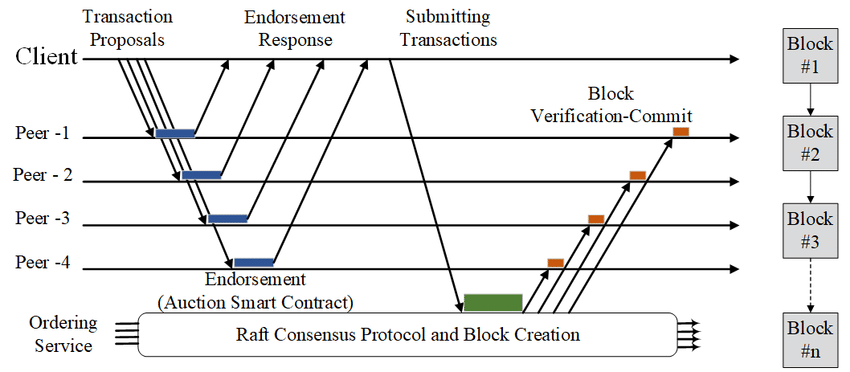
\includegraphics[width = 1\columnwidth]{images/methodology/TransactionFlow.jpg}
  \centerline{\includesvg[inkscapelatex=false, width=1\columnwidth]{images/methodology/TransactionFlow.svg}}
    \caption[Transaction flow in Hyperledger fabric]{Transaction flow in Hyperledger fabric}
    \label{fig:TransactionFlow.jpg}
\end{figure}

\textbf{Transaction initiation} \newline
Any transaction initiated by the gateway application targets the peers, who are the representative of the respective gateway applications. Peer of “Parichaya” is the target peer for the gateway application of “Parichaya” and Peer of “Nepal Government” is the target peer for the gateway application of “Nepal Government”.

For this, a transaction proposal is constructed first. The proposal is a request to invoke a chaincode function with certain input parameters, with the intent of reading and/or updating the ledger. The gateway application leveraging the Node SDK provided by hyperledger fabric utilizes one of the available API’s to generate the transaction proposal.

The SDK serves as a shim to package the transaction proposal into the properly architected format (protocol buffer over gRPC) and takes the application’s cryptographic credentials to produce a unique signature for this transaction proposal. The SDK submits the transaction proposal to a target peer, which will manage the transaction submission on behalf of the gateway application. The target peer first forwards the transaction proposal to other peers for execution, as required by the endorsement policy.\\ \newline

\textbf{Verification of Signature and Execution of transaction by Endorsing Peers} \newline
Both the endorsing peers, “Parichaya” and “Nepal Government” verify that the transaction proposal is well formed,  it has not been submitted already in the past (replay-attack protection),  the signature is valid (using the MSP), and  that the submitter (Gateway Application) is properly authorized to perform the proposed operation on that channel (digital\_identity channel). The endorsing peers take the transaction proposal inputs as arguments to the invoked chaincode’s function. The chaincode is then executed against the current state database to produce transaction results including a response value, read set, and write set (i.e. key/value pairs representing an identity document to create or update). No updates are made to the ledger at this point. The set of these values, along with the endorsing peer’s signature is passed back as a “proposal response” to the target peer.

\textbf{Inspection of proposal responses} \newline
The target peer verifies the proposal responses are the same prior to proceeding with the transaction submission. The architecture is such that even if a transaction is submitted without this check, the endorsement policy will still be checked and enforced when each peer validates transactions prior to committing them in the ledger.

\textbf{Assembly of endorsements into a transaction by target peer} \newline
The target peer “broadcasts” the transaction proposal and response within a “transaction message” to the ordering service. The transaction contains the Channel ID, the read/write sets, and a signature from each endorsing peer. The ordering service does not need to inspect the entire content of a transaction in order to perform its operation, it simply receives transactions, orders them, and creates blocks of transactions per channel.

\textbf{Transaction validation and commitment} \newline
The blocks of transactions are “delivered” to all peers on the channel. The transactions within the block are validated to ensure endorsement policy is fulfilled and to ensure that there have been no changes to ledger state for read set variables since the read set was generated by the transaction execution. Transactions in the block are tagged as being valid or invalid.\\\\

\textbf{Ledger update} \newline
Each peer appends the block to the channel’s chain, and for each valid transaction the write sets are committed to the current state database. An event is emitted by each peer to notify the gateway application that the transaction (invocation) has been immutably appended to the chain, as well as notification of whether the transaction was validated or invalidated.




\subsection{Implementation Details of Karmachari Web App}
\vspace{15pt}
    \begin{figure}[H]
\centerline{\includesvg[inkscapelatex=false,width=1\columnwidth]{images/methodology/KarmachariUsecase.svg}}
\caption{Use case Diagram of Karmachari Web App}

\label{fig: KarmachariUsecase.svg}
\end{figure}


Karmachari Web App provides an interface for the government officials to record and update the identity details of the users in the private blockchain. Initially, the users need to log in with their username and password. The credentials provided are then verified by the backend server before the user gets access to the main dashboard. Once the user is logged in, they can register the National Identity, Citizenship and Driving License of the users. They can also search for the required documents using the National Identity Number linked with it. Moreover, the users can update the searched document if necessary. \\\\
    

\textbf{Authentication}\newline
    Authentication process of the government officials on the web application is based on JWT authentication. For the login process in the web app, the user is required to input their username and password. The credentials are then forwarded to the node backend server for authentication through an API request. The backend server verifies the credentials and generates a JWT which is then returned back to the user as a response. On receiving the token, the user is logged in to the web application. The web app then attaches this authentication token with all other subsequent requests made by the web app to the backend.

\textbf{Registration of Documents} \newline
The government officials, after authentication, can fill the documents of the users on the Karmachari web app for registration. Initially, the officials have to fill the forms of national identity documents among others, as it acts as a base for all other documents. The form is validated during the filling process itself. The Karmachari web app then sends the document details to the Fabric gateway, which invokes a function on the smart contract to register the national identity document. However, for other documents, the government officials have to first enter the associated National Identity Number, The karmachari web app sends this number to the Fabric gateway which invokes a function on smart contract to check where the received National Identity Number exists on the blockchain or not. If it exists, the government officials are able to fill the form. Again, the form is validated during the process. Finally, the Karmachari web app sends the document details to the Fabric gateway, which invokes a function on the smart contract to register the required document.
    \begin{figure}[H]
\centerline{\includesvg[inkscapelatex=false,width=0.45\columnwidth]{images/methodology/RegisterNID.svg}}
\caption{Register NID}

\label{fig: example}
\end{figure}
   \begin{figure}[H]
\centerline{\includesvg[inkscapelatex=false,width=0.45\columnwidth]{images/methodology/RegisterLicense.svg}}
\caption{Register License}

\label{fig: RegisterLicense.svg}
\end{figure}

   \begin{figure}[H]
\centerline{\includesvg[inkscapelatex=false,width=0.45\columnwidth]{images/methodology/RegisterCitizenship.svg}}
\caption{Register Citizenship}

\label{fig: example}
\end{figure}

   
\textbf{Searching and Updating Documents}\newline
To search for any documents in the web app, the user needs to provide the National Identity Number of the user and select the document type the user is searching for. The web app then sends an API request to the backend server to check if the document exists, which in turn invokes a smart contract function in the blockchain through gRPC to check if the document exists. A response is then sent back to the web app. If the document exists, the details of the document are shown to the user. Else, an error is shown. The user can also update the details of the shown document if necessary. If the details are updated, the updated details are sent to the backend server which then overwrites the details of the document stored in the blockchain by invoking a smart contract function.\newline
Government official’s authentication on the web application is based on JWT authentication. The user inputs their username and password which is forwarded to the node backend server. The server verifies the credentials and generates a JSON Web Token. The server provides the token to the user as a response and the user is logged in to the web application. The user can then fill the forms (National Identity) of users into the blockchain storage through the server.
\begin{figure}[H]
\centerline{\includesvg[inkscapelatex=false,width=0.45\columnwidth]{images/methodology/SearchAndUpdate.svg}}
\caption{Search And Update Documents}

\label{fig: SearchAndUpdate.svg}
\end{figure}

\subsection{Implementation Details of Parichaya app}
\vspace{15pt}
\begin{figure}[H]
\centerline{\includesvg[inkscapelatex=false,width=1\columnwidth]{images/methodology/MobileUsecase.svg}}
\caption{Use Case Diagram of Parichaya App}
\label{fig: MobileUsecase.svg}
\end{figure}
Parichaya Mobile App provides an interface for users to view and share their identity document details. The user requires to be authenticated in the mobile app through their National Identity Number and mobile number.This process includes the user receiving an OTP in their registered mobile number. The user is authenticated if the input OTP is verified by the backend server. After authentication, users can view their government issued documents, online or offline. Moreover, users can share their identity details to other users or third party applications through QR code. Consequently, the users can also view other user’s identity details by scanning the QR code using the application’s scanner.\\ \\ 

\textbf{Authentication} \newline
The authentication process begins when the user provides their National Identity Number to the mobile app. The number is then forwarded to the Parichaya backend server and subsequently to the Fabric gateway application. The Fabric gateway invokes a function in the smart contract providing the number it received from the user. The function checks if the number exists in the blockchain and returns a response to the Fabric gateway. The response traverses all the way back to the mobile application, which shows an error or shows the next step of the authentication process depending on the response. The user then provides their Mobile Number, associated with their National Identity Card. The mobile number and the national identity number are forwarded to the Parichaya backend server, which requests for the National Identity Details of the given NIN to the Fabric gateway. The gateway invokes another function which provides the National Identity Details of the given NIN. This response traverses back to the Parichaya backend, where the mobile number it received is compared with the one in the National Identity Details. This is to check that the mobile number being used is indeed the mobile number that is linked with the National Identity Card. If it is verified, then an OTP is generated and sent to the given mobile number. The user is required to input the OTP, which is forwarded to the Parichaya backend. If the OTP is verified, an auth token is generated and sent as the response to the mobile app. The received token is then stored in the mobile database as all the future interactions with the Parichaya backend requires it for authentication. Finally, for app lock purposes, the user is required to set up a four digit pin code, which is stored in the mobile database as well. After the completion of each of these steps, the user is finally logged in to the mobile app.
    
\textbf{Fetching Documents}\newline
In the first login, a request for the government issued documents is sent to the Parichaya backend, including the NIN and the auth token. If the token has not expired, the same request is sent to the Fabric gateway. This invokes a function which returns a response containing all the available documents associated with the NIN. After the Parichaya backend obtains the response, it creates card images of each of the documents, front and back, for a better visual representation. The mobile app finally receives the documents along with the document images. The received documents and images are stored in the mobile database for offline viewing. Current date and time of the fetch request is also stored to sync the data in the mobile database with the data in the blockchain.\newline
For other subsequent logins, the user just has to input the pin code that was previously set. Users can also opt to enable biometric login options, which can be enabled from the settings of the mobile app. After verification, if there is no internet connection, the documents stored in the mobile database are shown, else if there is internet connection, then a syncing process is initiated. The syncing process starts by requesting for the last updated date and time of documents to the Parichaya backend, which includes sending the NIN and the auth token. If the token is valid, the mobile app acquires the date and time of the last update, which is compared to the one stored in the mobile database. If the mobile stored date and time is more recent than the fetched date and time, the currently stored documents in the mobile app are shown, else the process of document fetch is initiated.
  \begin{figure}[H]
\centerline{\includesvg[inkscapelatex=false,height=0.6\paperheight]{images/methodology/MobileActivity.svg}}
\caption{Activity Diagram Of Login Process in Parichaya App}

\label{fig: MobileActivity.svg}
\end{figure}
  \begin{figure}[H]
\centerline{\includesvg[inkscapelatex=false,width=1\columnwidth]{images/methodology/MobileAuthenticationSequence.svg}}
\caption{Authentication and Data Fetching Process in Parichaya App}

\label{fig: example}
\end{figure}


\textbf{Sharing Identity Details to Third Party Application} \newline
To send details to the third party web client, the user has to click on the apply with Parichaya button. This initiates a websocket connection between the web client and the Parichaya backend server. However, the web client has to be registered into the backend with their name, domain, logo and requesting identity fields. In other words, the backend has to recognize the third party client application before it can make a websocket connection. Otherwise, the request to establish the websocket connection is rejected by the Parichaya backend. After the initialization of websocket connection, the Parichaya backend responds with the request id. The web client generates a QR code using this request id. The user requires the Parichaya mobile app to scan the QR code, and once the QR code is scanned, the Parichaya app requests the Parichaya backend with the obtained request id for the details of the document requester and the requested fields. This is for the full transparency of the users data being shared. The user then chooses to either approve or deny this request after viewing the details of the document requester and the requested fields. If the user chooses to deny the request, the websocket connection closes by sending a denied message to the web client. If the user chooses to approve the request, the Parichaya backend requests for all the required user details to the Fabric gateway which invokes a function in the smart contract that responds with the required details. Finally, the Parichaya backend sends the user’s details to the web client. The websocket connection is then closed with an approved request message shown on the Parichaya app. \\


\begin{figure}[H]
\centerline{\includesvg[inkscapelatex=false,width=1\columnwidth]{images/methodology/ThirdpartyQRSequence.svg}}
\caption{Sharing Identity Details to Third Party Application}

\label{fig: ThirdpartyQRSequence.svg}
\end{figure}

\textbf{Sharing Identity Details to Other Parichaya App Users} \newline
Users can send either their verified age or driving license to other Parichaya app users. To send the details, the user needs to click on the generate QR code button on either one of the documents. This will initiate a websocket connection between the Parichaya app and the Parichaya backend server. After initialization, the Parichaya app sends a request including the type of document required to the Parichaya backend, which in turn responds with a permit id. A QR code is generated with the received permit id. Other users can scan the QR code to get the permit id. The receiving user’s Parichaya app then proceeds to get a request for the document details with the permit id  and the auth token to the Parichaya backend. The Parichaya backend then verifies the permit id and the token, and proceeds to send the request for the required document to the Fabric gateway application. This invokes a function in the smart contract which responds with the required documents, and it is traversed back to the Parichaya backend. The document details are sent to the receiving user, and the receiving user’s name is sent to the primary user. After the details have been shared, the user can exit the page, which closes the websocket connection.
\begin{figure}[H]
\centerline{\includesvg[inkscapelatex=false,width=1\columnwidth]{images/methodology/QRToShareSequence.svg}}
\caption{Sharing Identity Details to other Parichaya App User}

\label{fig: QRToShareSequence.svg}
\end{figure}


% \section{Dataset Explanation}

% \section{Description of Algorithms}



% \section{Verification and Validation Procedures}
\chapter{RESULTS AND ANALYSIS}


% (20\% of Report Length)

% a. Showcase the output at various intermediate stages of the project pipeline

% b. Use proper data visualizing techniques to present the output

% c. Figures and tables must be accompanied by an explanation

\section{User Interface}

\subsection{Mobile Application}

\textbf{Initial Login}\\
Initially, a user should provide National Identity Number along with the Mobile Number that is linked to their National Identity Card.
\begin{multicols}{2}
        \begin{figure}[H]
        \centering
        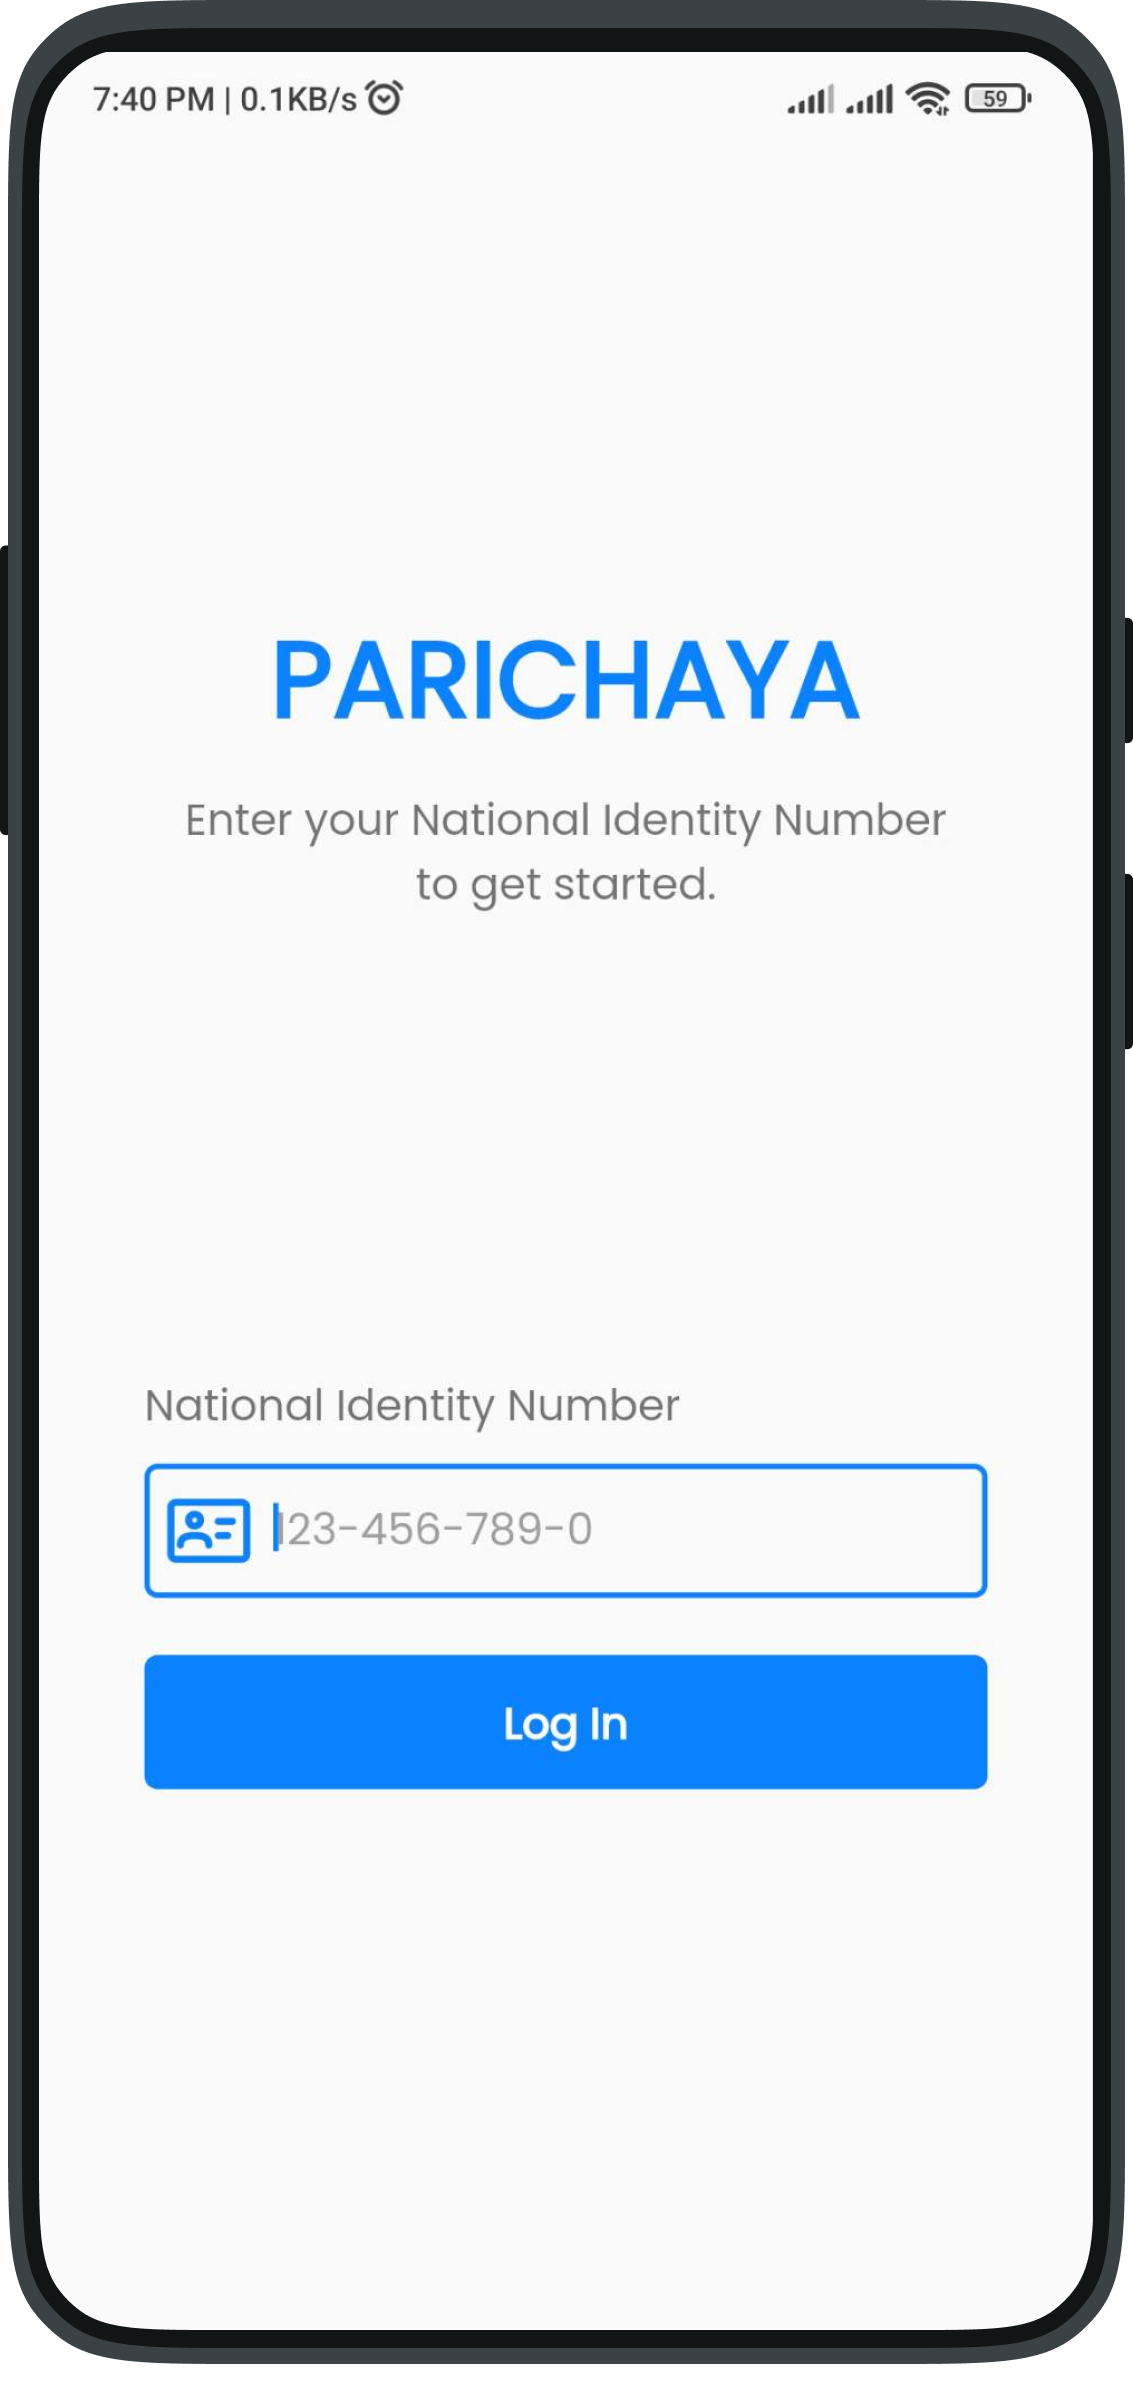
\includegraphics[width=0.6\linewidth]{images/results/mobile/LoginNIN.png}
        \caption[Enter NIN Screen]{Enter NIN Screen}
        \label{fig:LoginNIN.png}
        \end{figure}

      \begin{figure}[H]
            \centering
            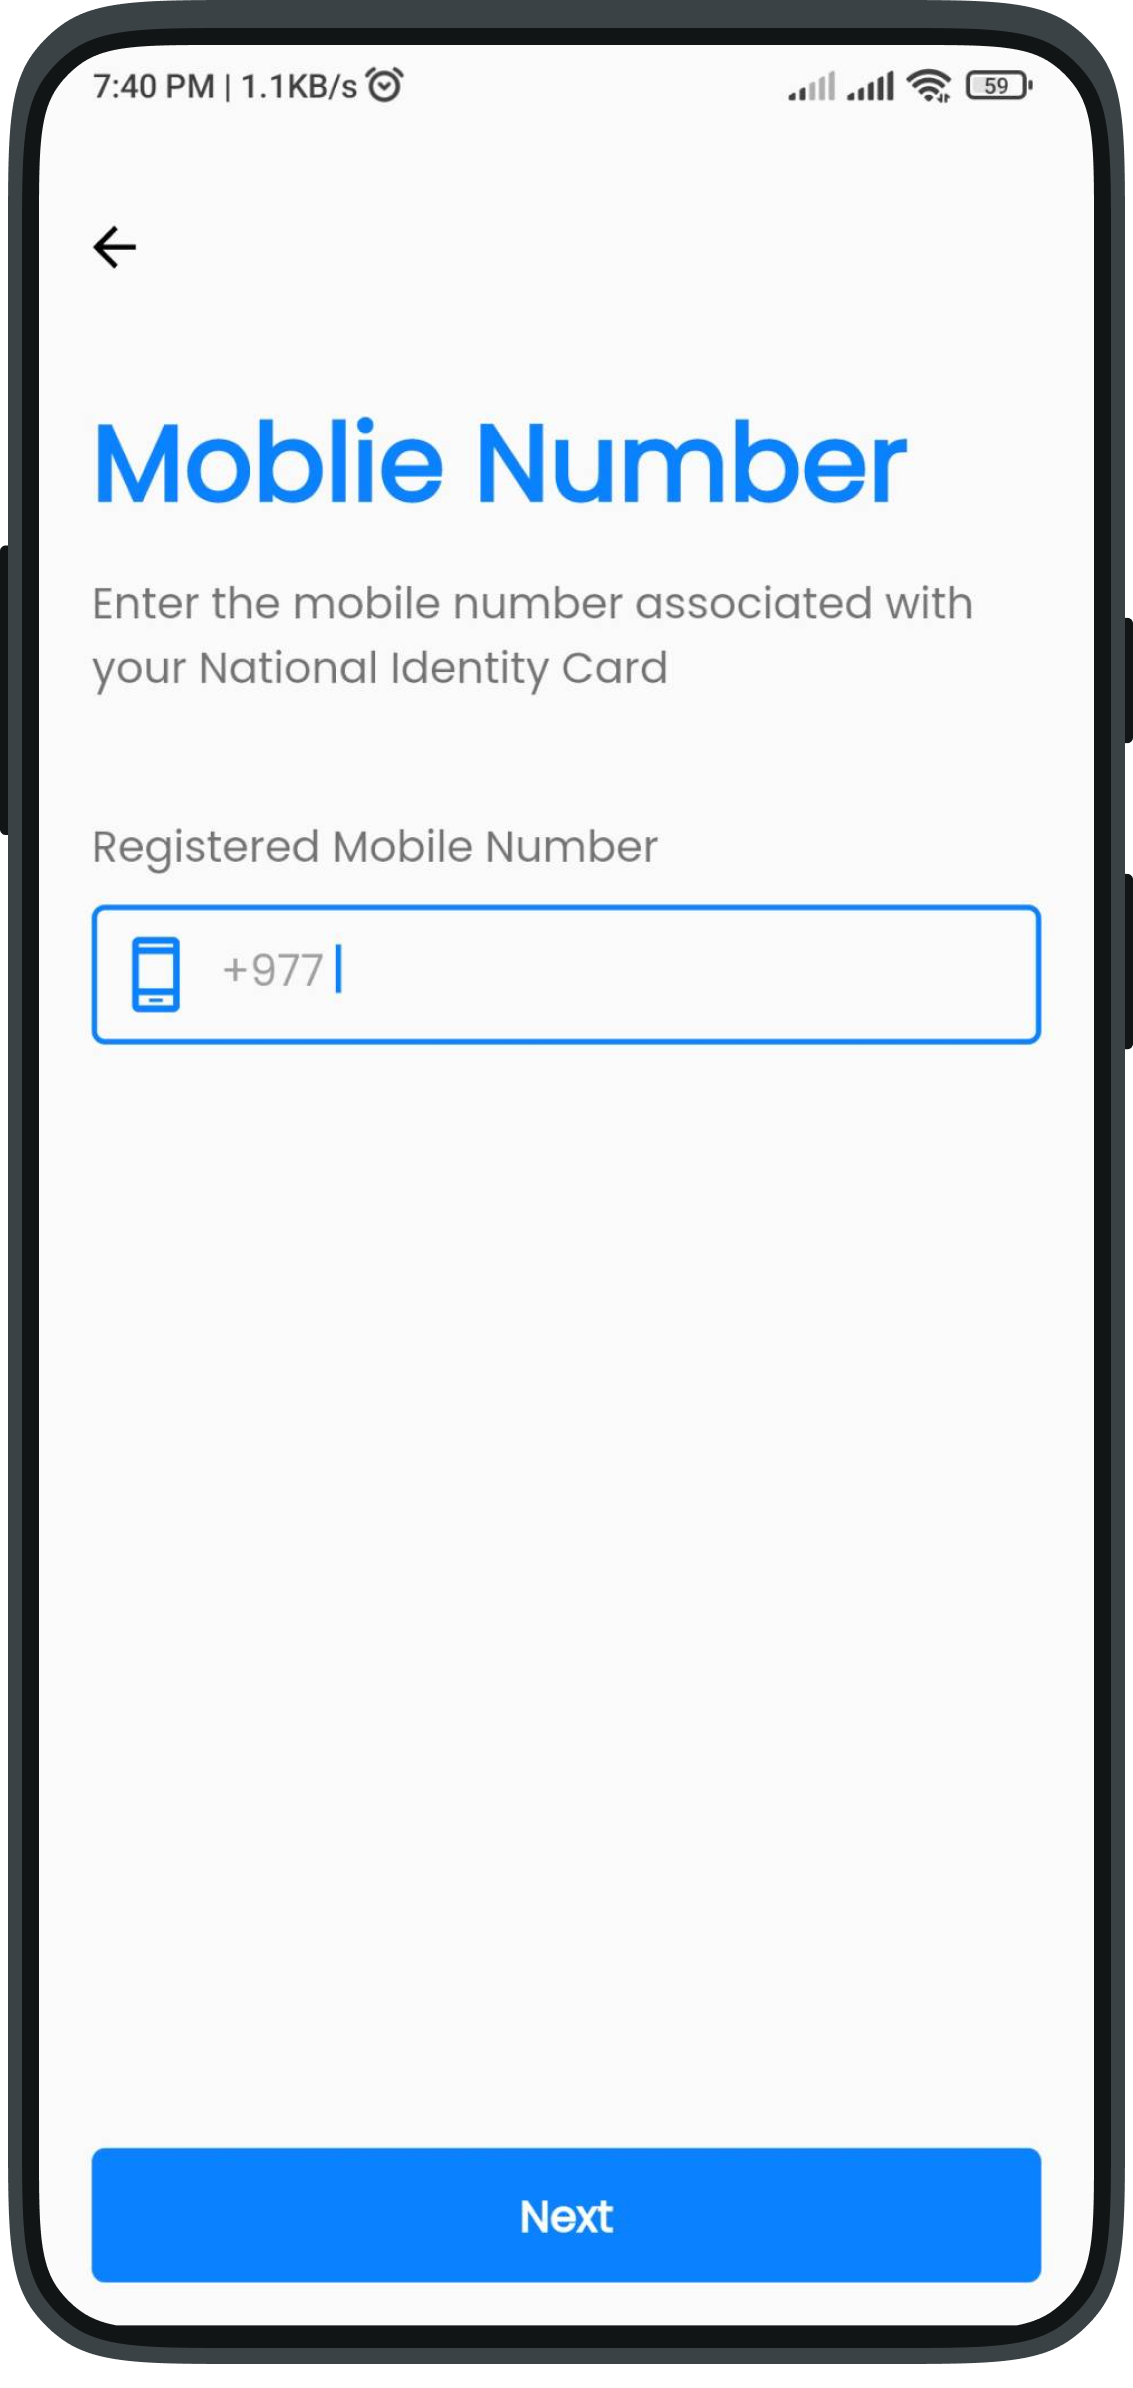
\includegraphics[width=0.6\linewidth]{images/results/mobile/MobileNumber.png}
            \caption[Enter Mobile Number Screen]{Enter Mobile Number Screen}
            \label{fig:MobileNumber.png}
            \end{figure}
\end{multicols}
\textbf{OTP Verification}\\
    If both of the number exist, an OTP is sent to the mobile number given by the user for verification. In case of an error, OTP can be resent to the user. 
    \newpage
    \begin{multicols}{2}
        \begin{figure}[H]
        \centering
        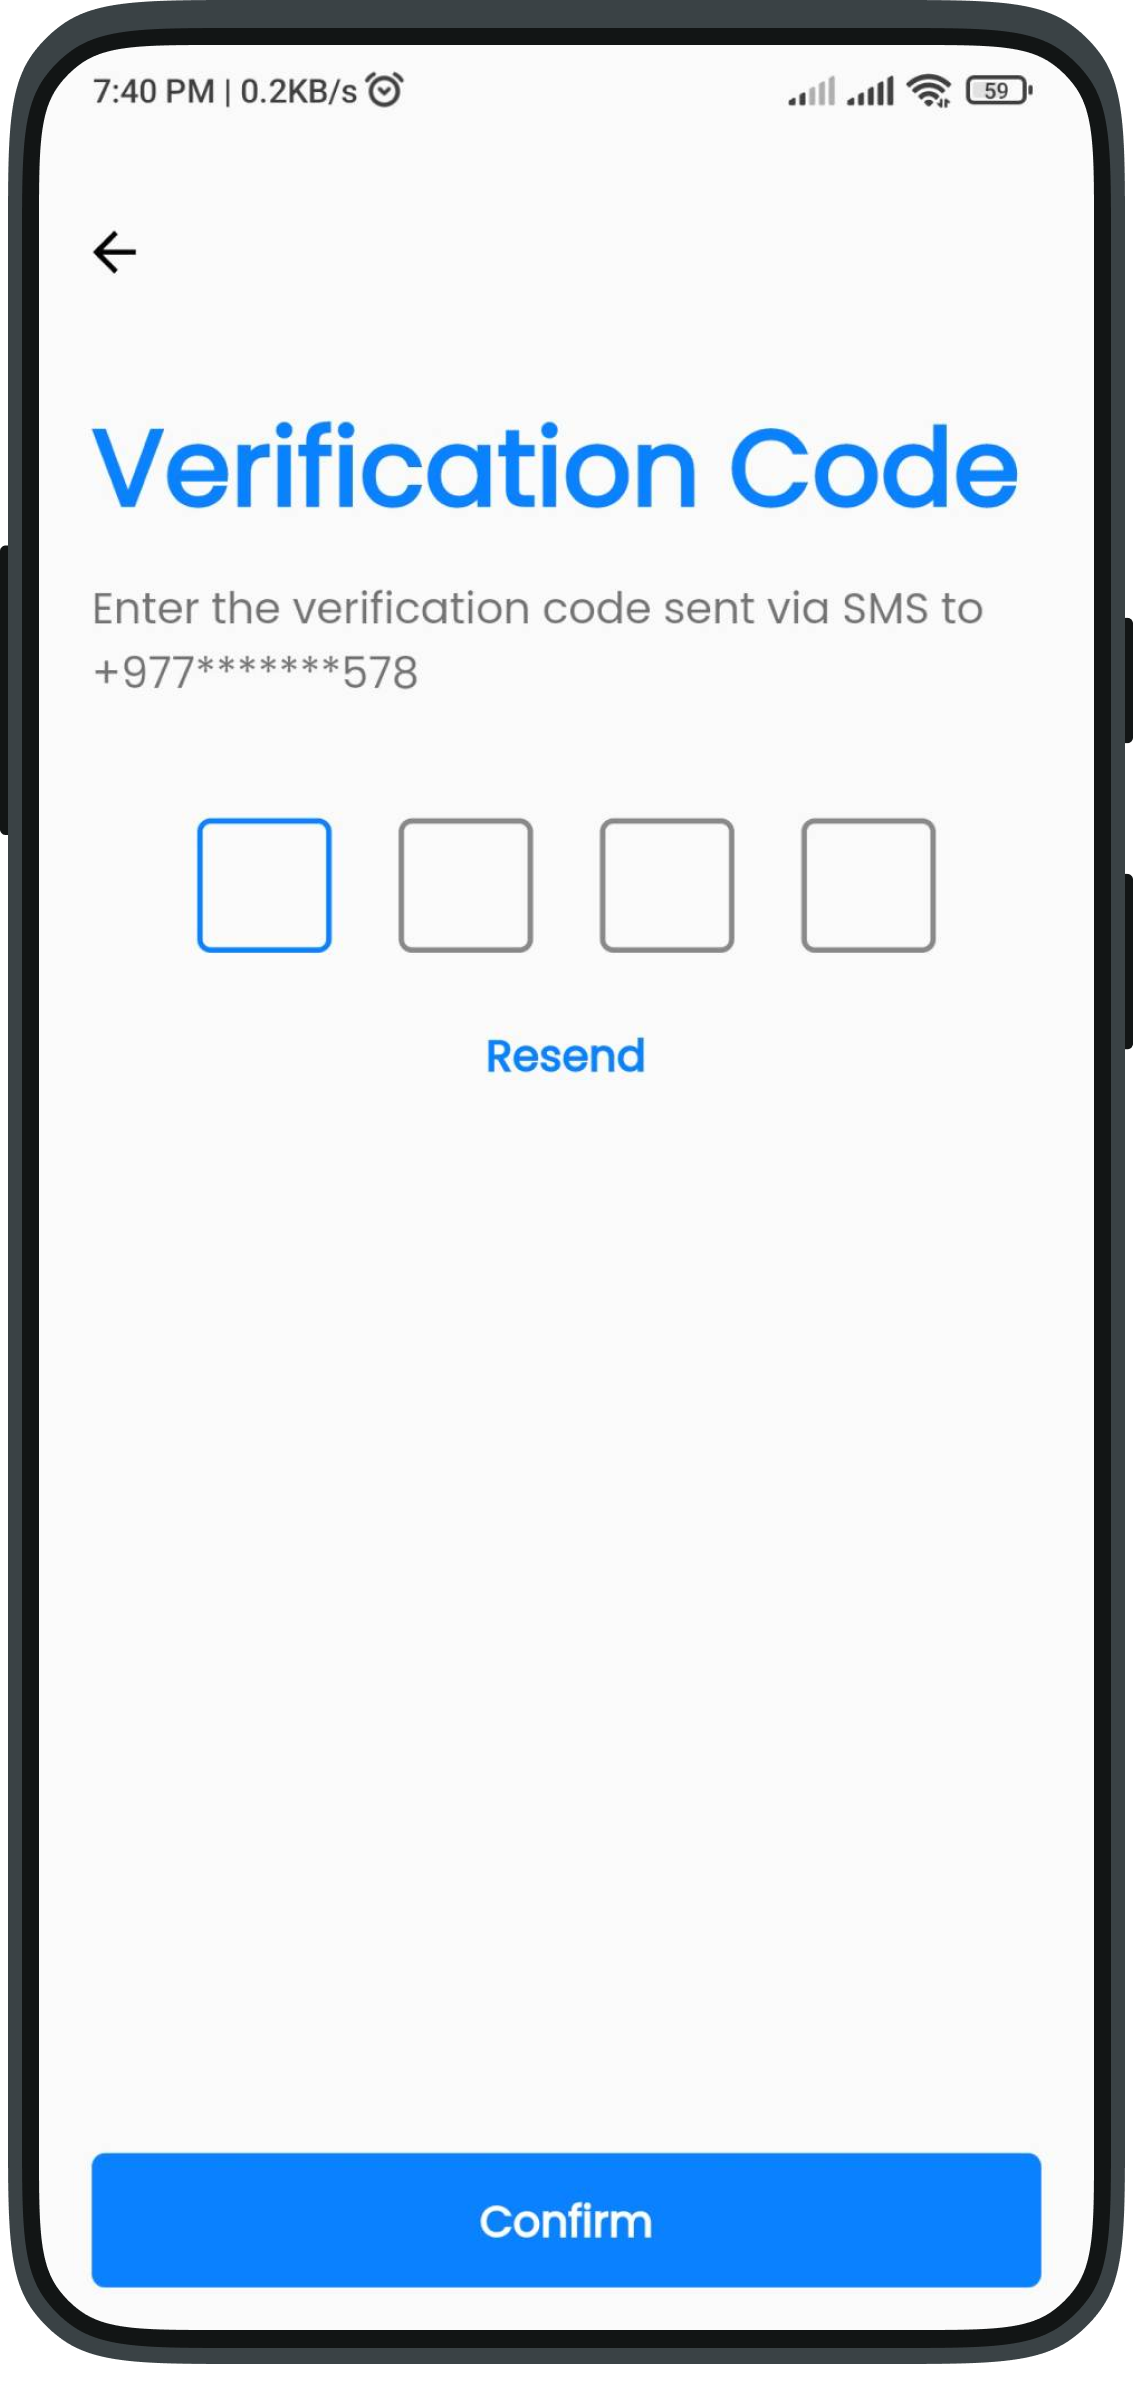
\includegraphics[width=0.6\linewidth]{images/results/mobile/OTP.png}
        \caption[Enter OTP Screen ]{Enter OTP Screen}
        \label{fig:OTP.png}
        \end{figure}
           \begin{figure}[H]
        \centering
        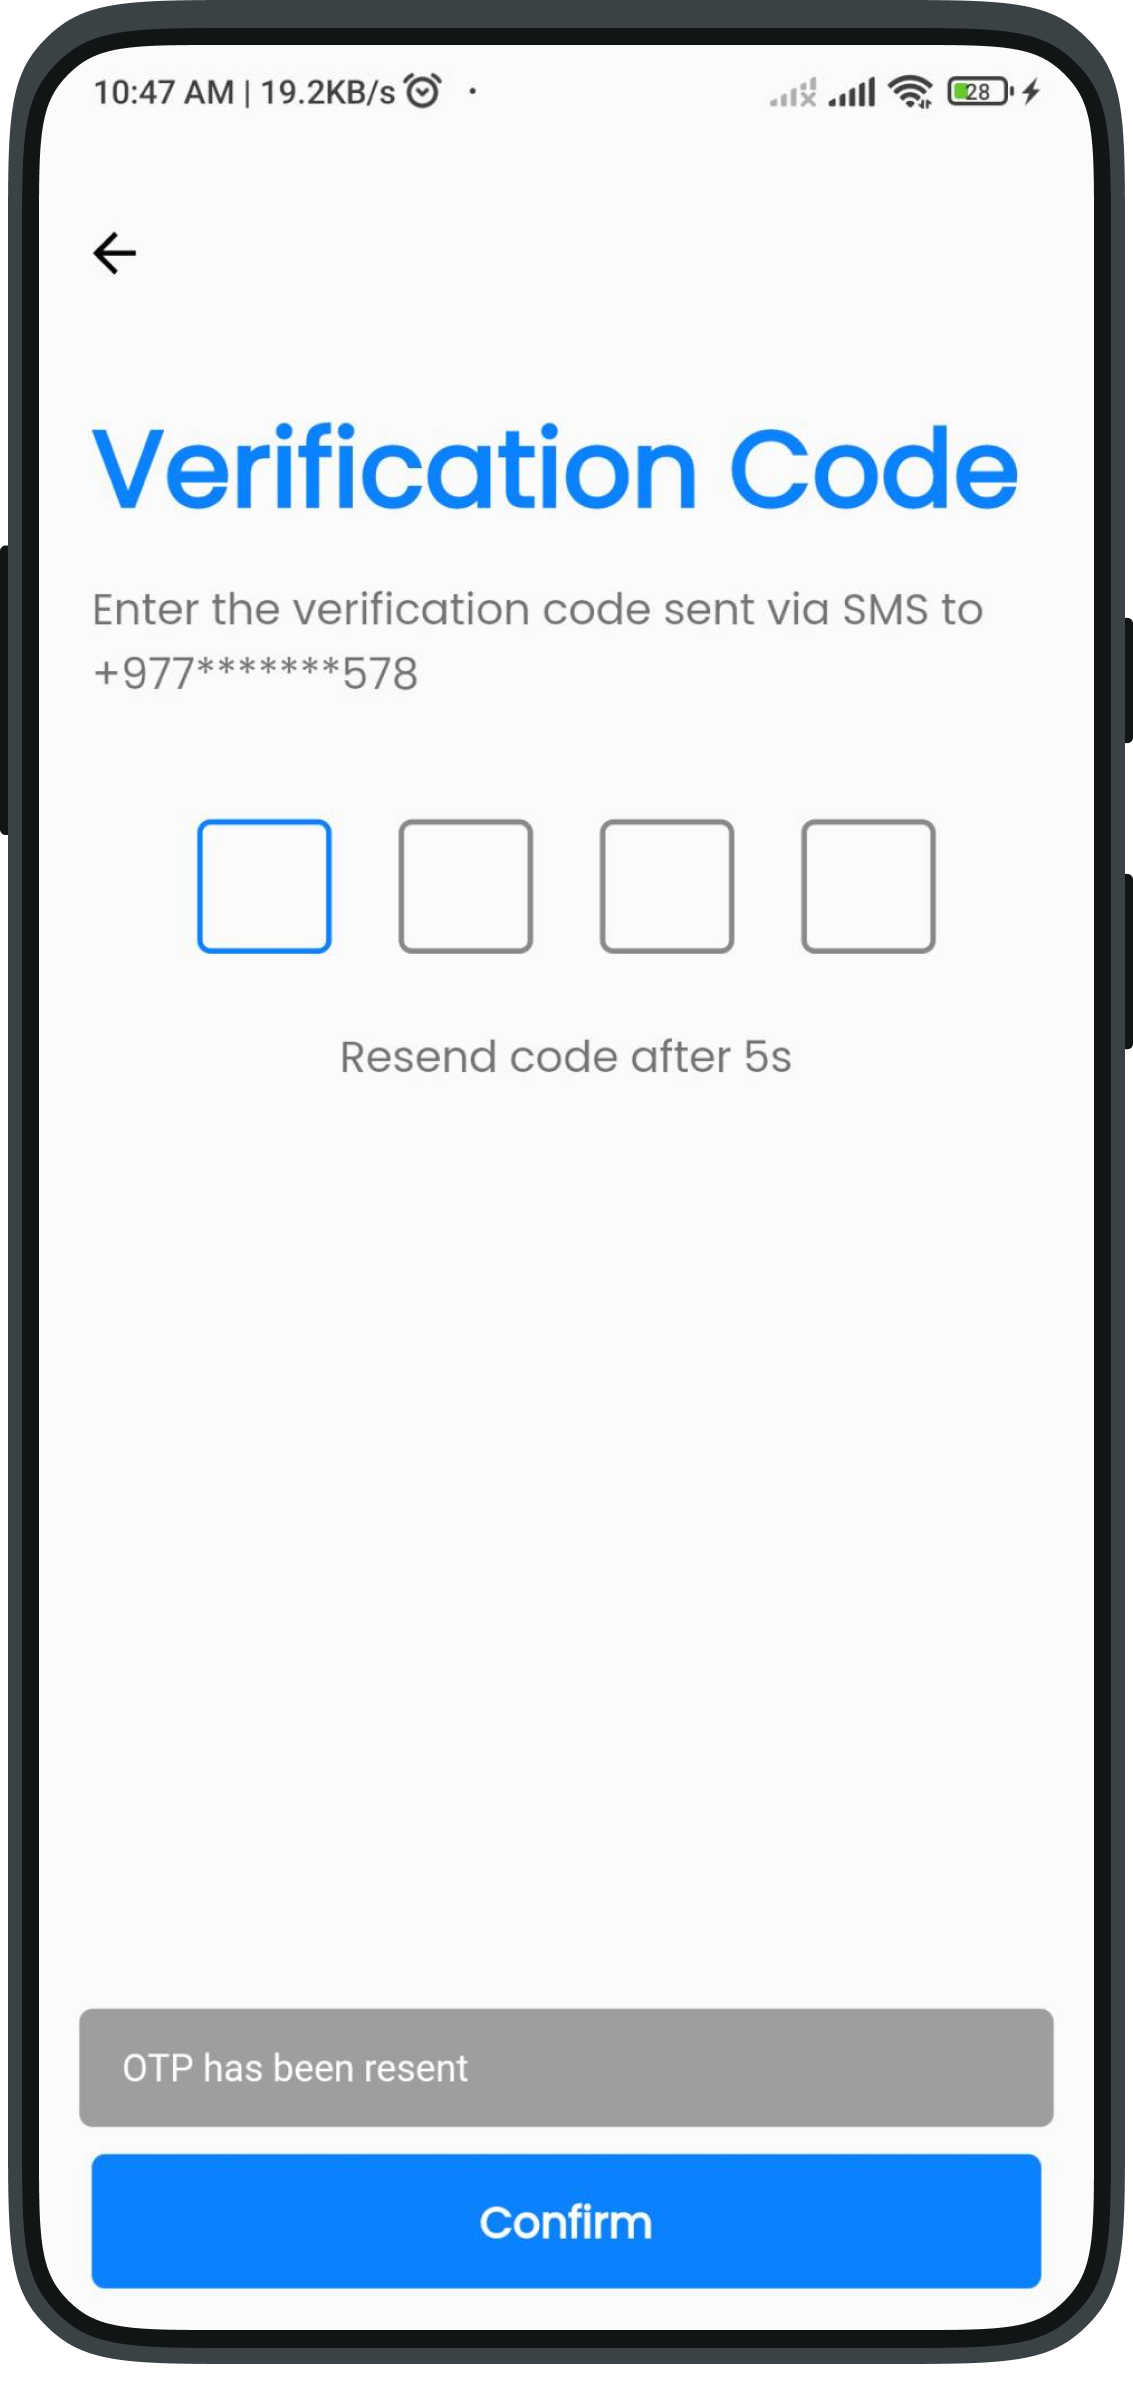
\includegraphics[width=0.6\linewidth]{images/results/mobile/OTPResend.png}
        \caption[Resend OTP Screen]{Resend OTP Screen}
        \label{fig:OTPResend.png}
        \end{figure}
        \end{multicols}

\textbf{Setting up MPIN}\\
    After validating the OTP, user can set up a pin which can be used for all other subsequent logins by the user.
    \begin{figure}[H]
    \centering
    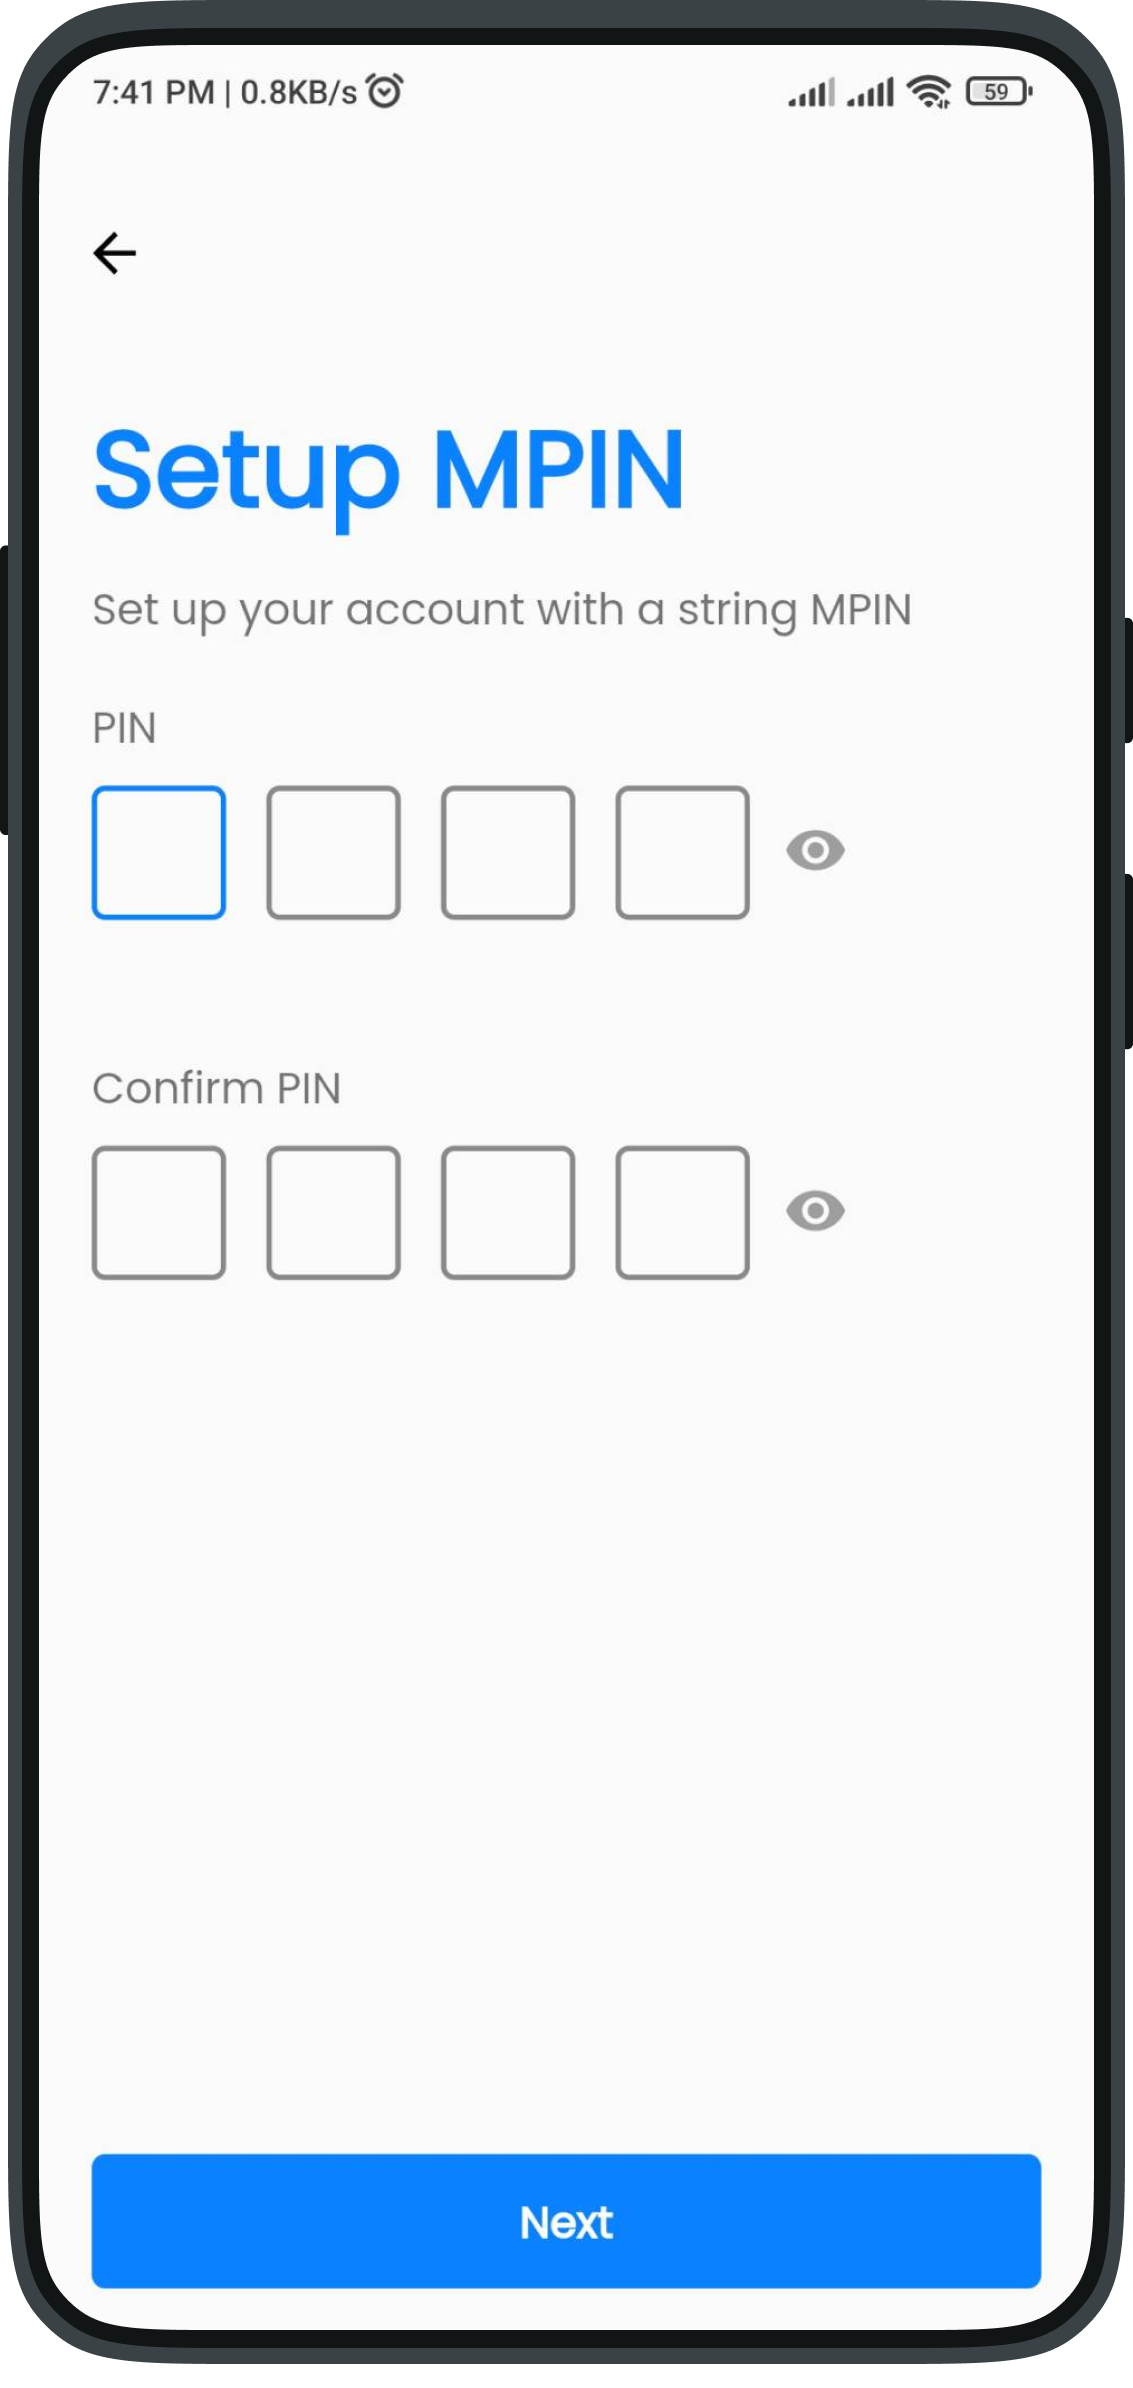
\includegraphics[width=0.3\linewidth]{images/results/mobile/SetupMPIN.png}
    \caption[Setup Pin]{Setup Pin}
    \label{fig:SetupMPIN.png}
    \end{figure}

\newpage
\textbf{Login with MPIN or Fingerprint}\\
    When user reopens the application, they are prompt to enter the mpin set during the initial login. They can also enable biometric login and use their fingerprint to login with instead of entering the mpin.
       \begin{figure}[H]
        \centering
        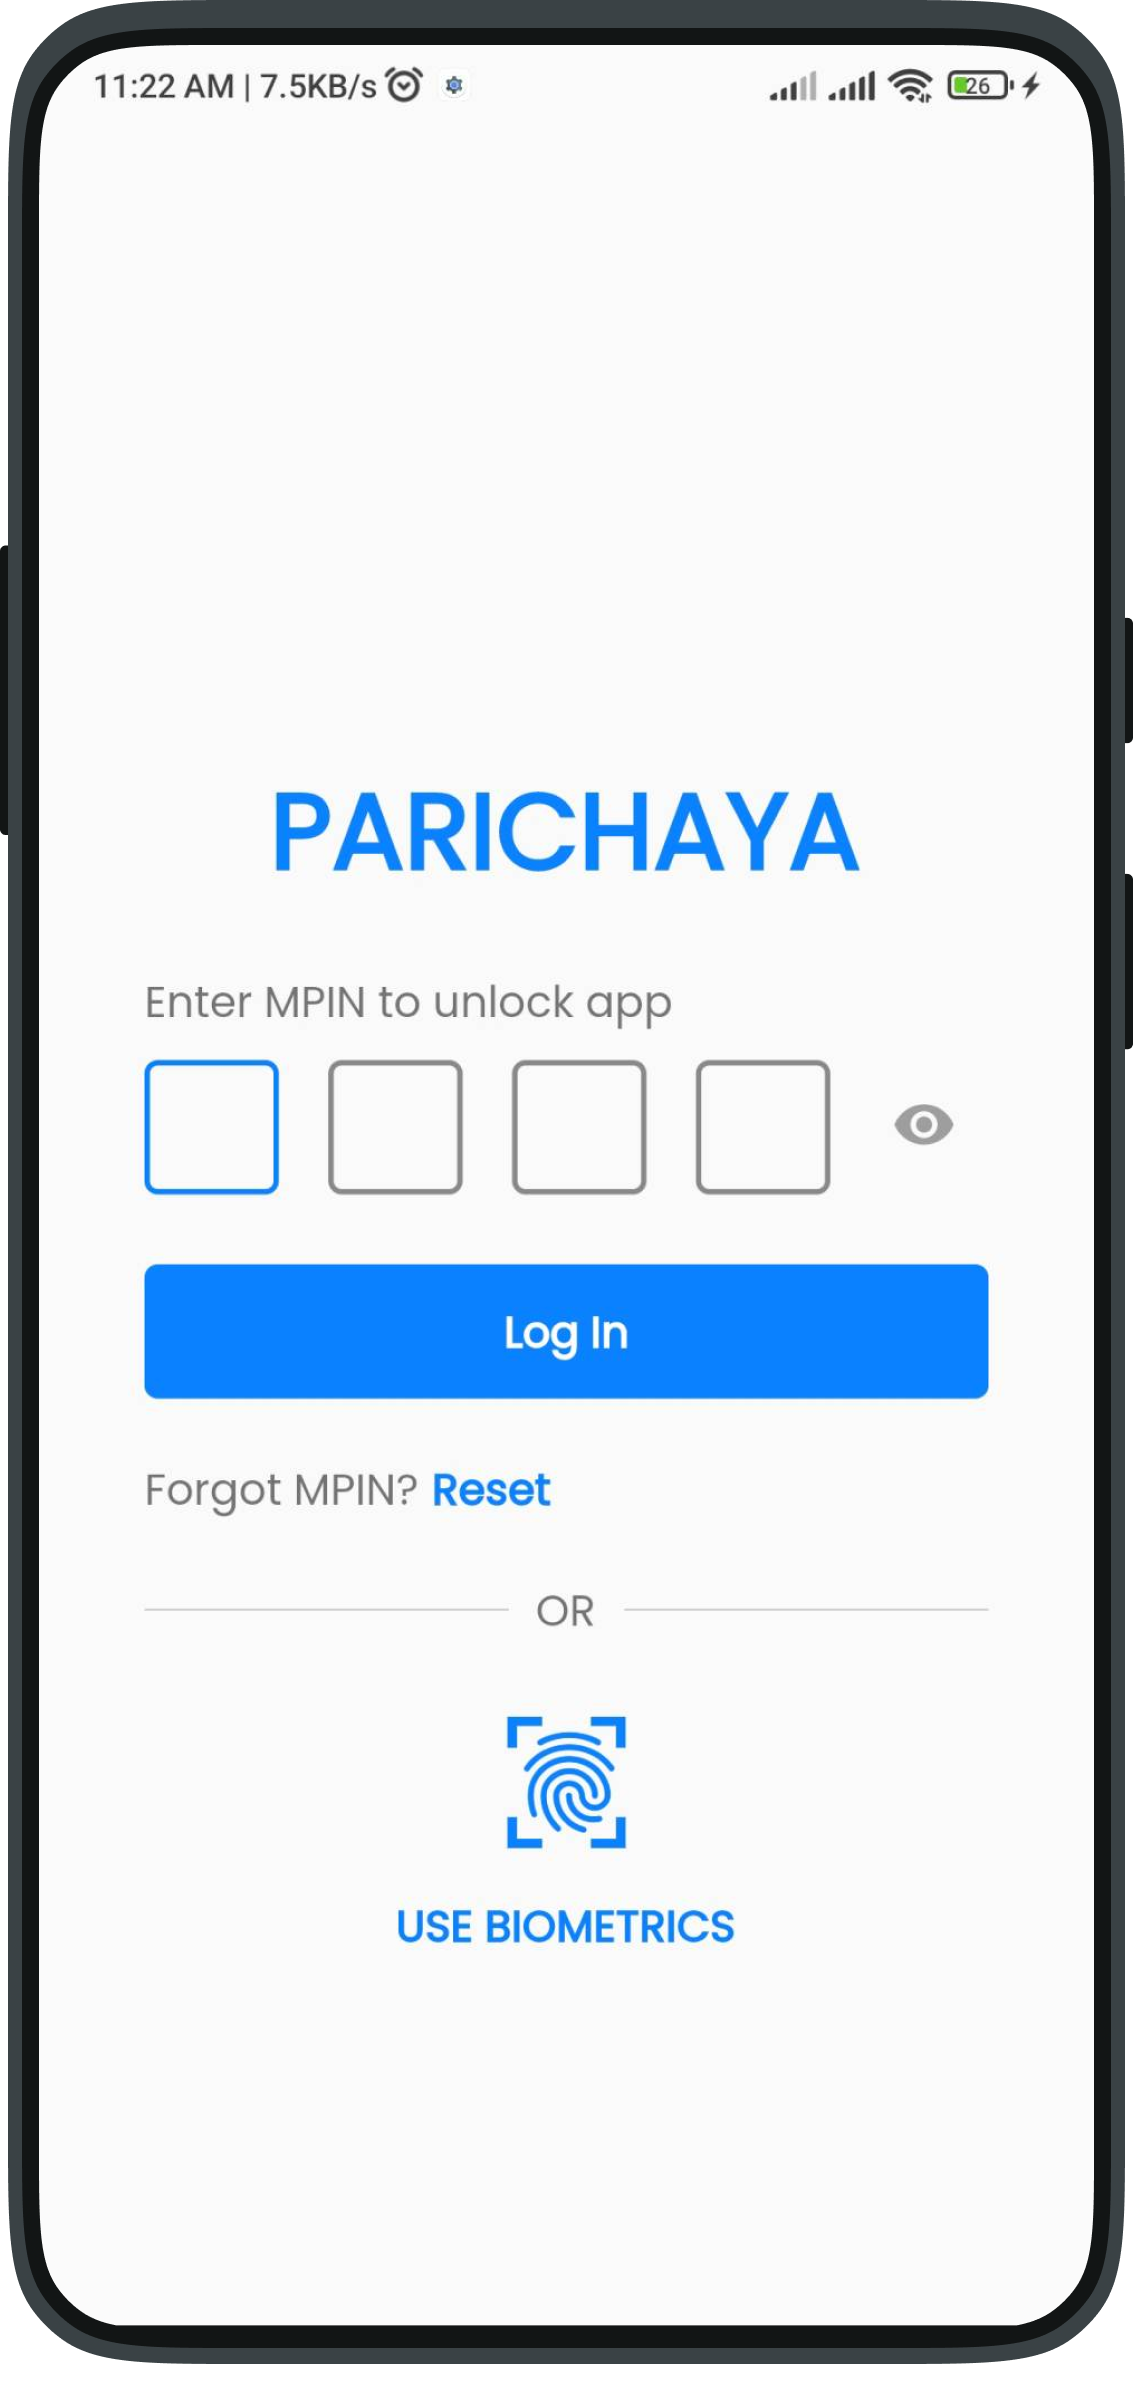
\includegraphics[width=0.3\linewidth]{images/results/mobile/LoginScreen.png}
        \caption[Login with MPIN Screen]{Login with MPIN Screen}
        \label{fig:LoginScreen.png}
        \end{figure}
    
\textbf{Forgot MPIN}\\
    In case the user forgets the mpin, they can opt to reset the mpin by entering the OTP sent to their mobile number. 
    \newpage
    \begin{multicols}{2} 
        \begin{figure}[H]
        \centering
        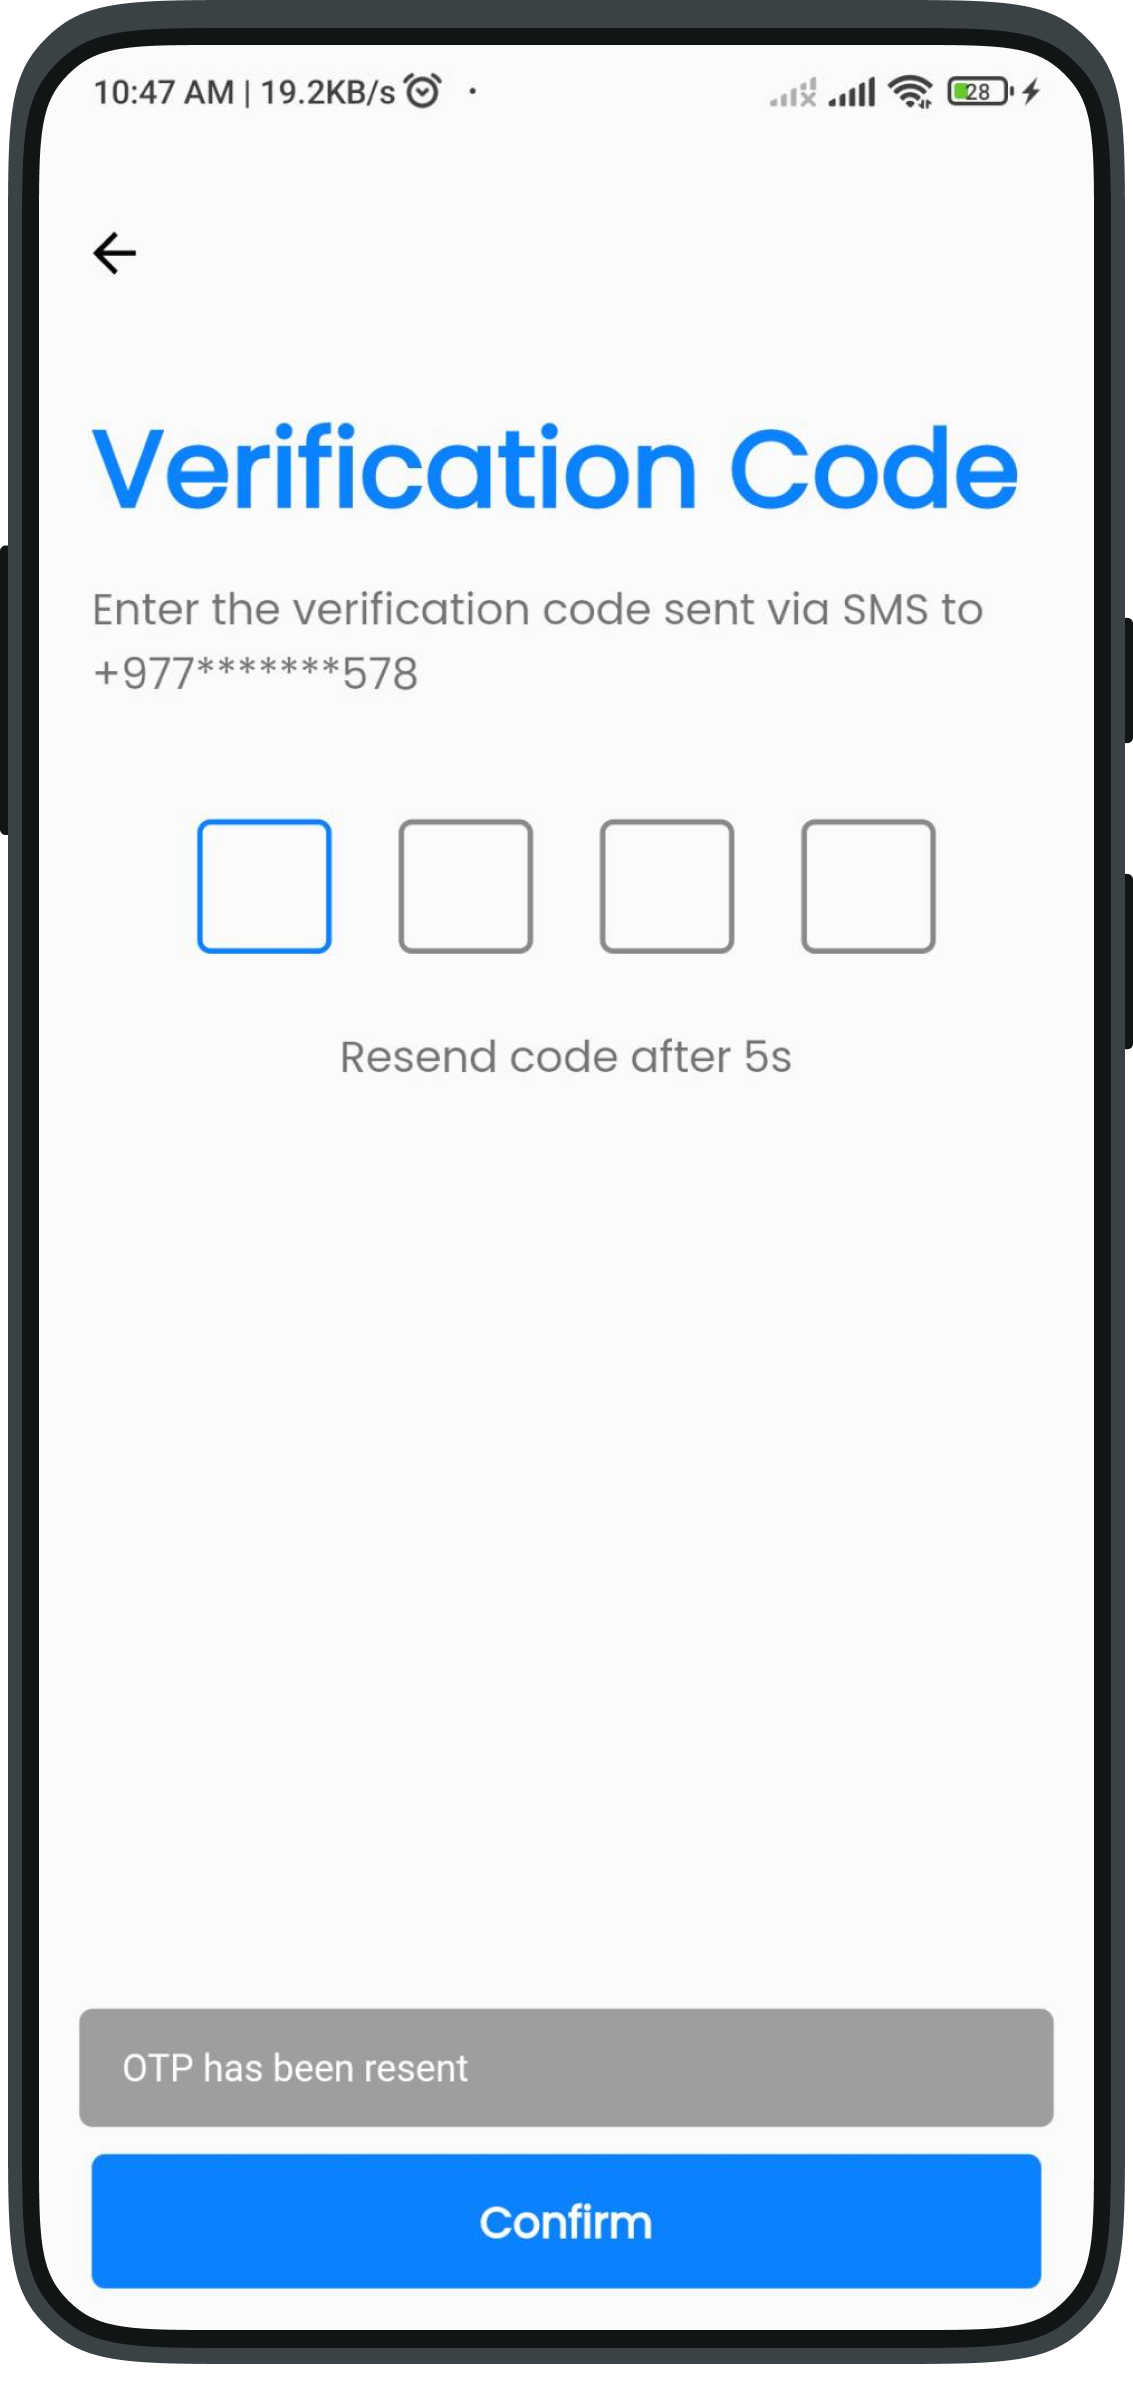
\includegraphics[width=0.6\linewidth]{images/results/mobile/OTPResend.png}
        \caption[Reset MPIN OTP Screen]{Reset MPIN OTP Screen}
        \label{fig:OTPResend.png}
        \end{figure}
        \begin{figure}[H]
        \centering
        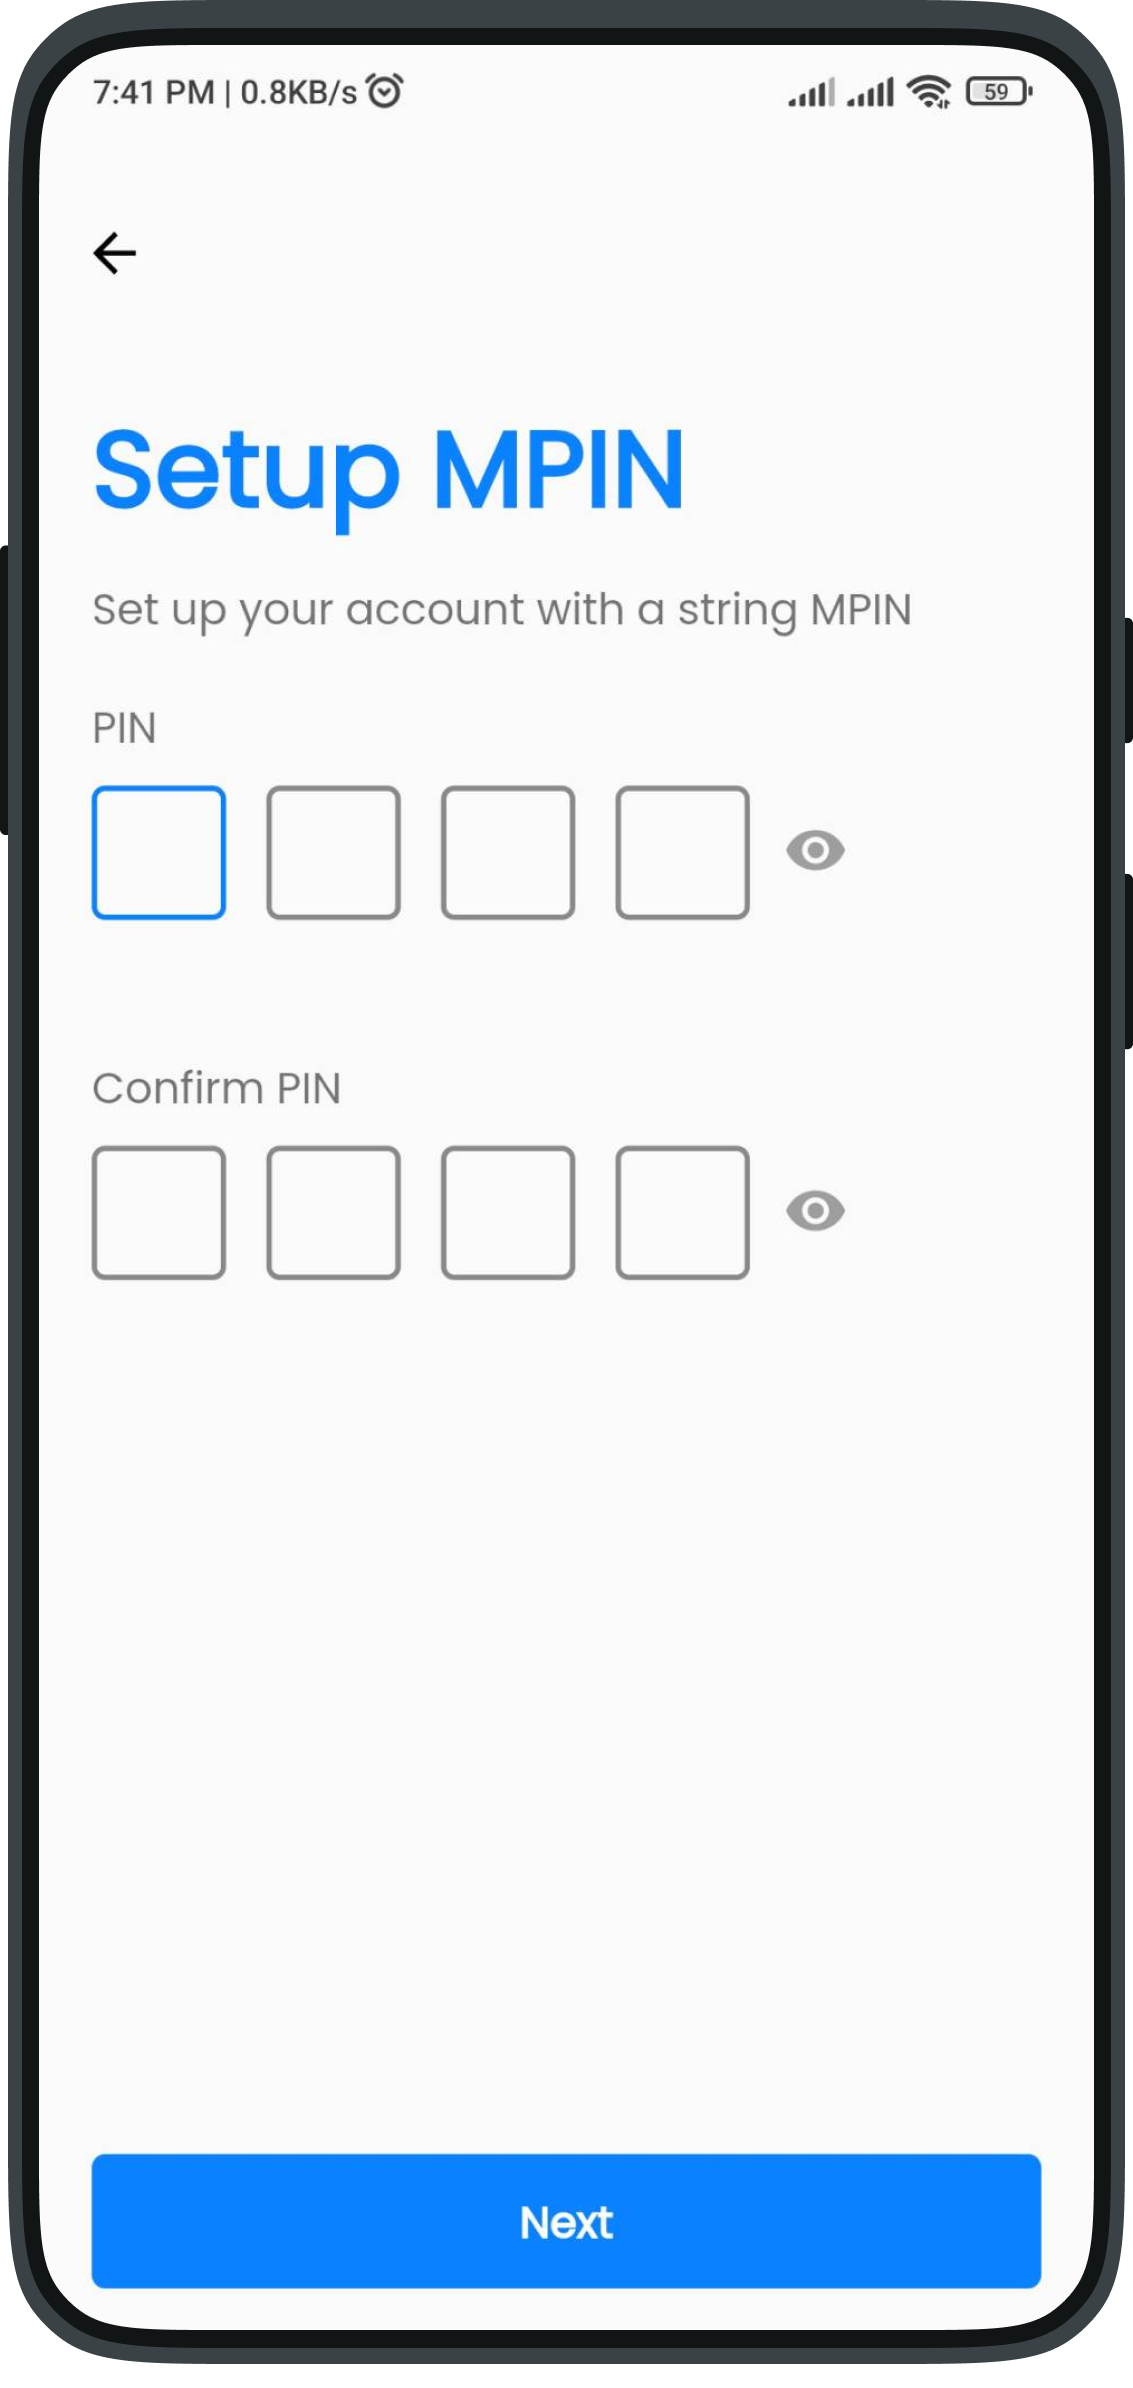
\includegraphics[width=0.6\linewidth]{images/results/mobile/SetupMPIN.png}
        \caption[Reset MPIN Screen]{Reset MPIN Screen}
        \label{fig:SetupMPIN.png}
        \end{figure}
      \end{multicols}
      
\textbf{Document View}\\
After completion of login process, user is navigated to the homescreen. Here, user can view the details of their documents and it's related card images.
\begin{multicols}{2}
    \begin{figure}[H]
        \centering
        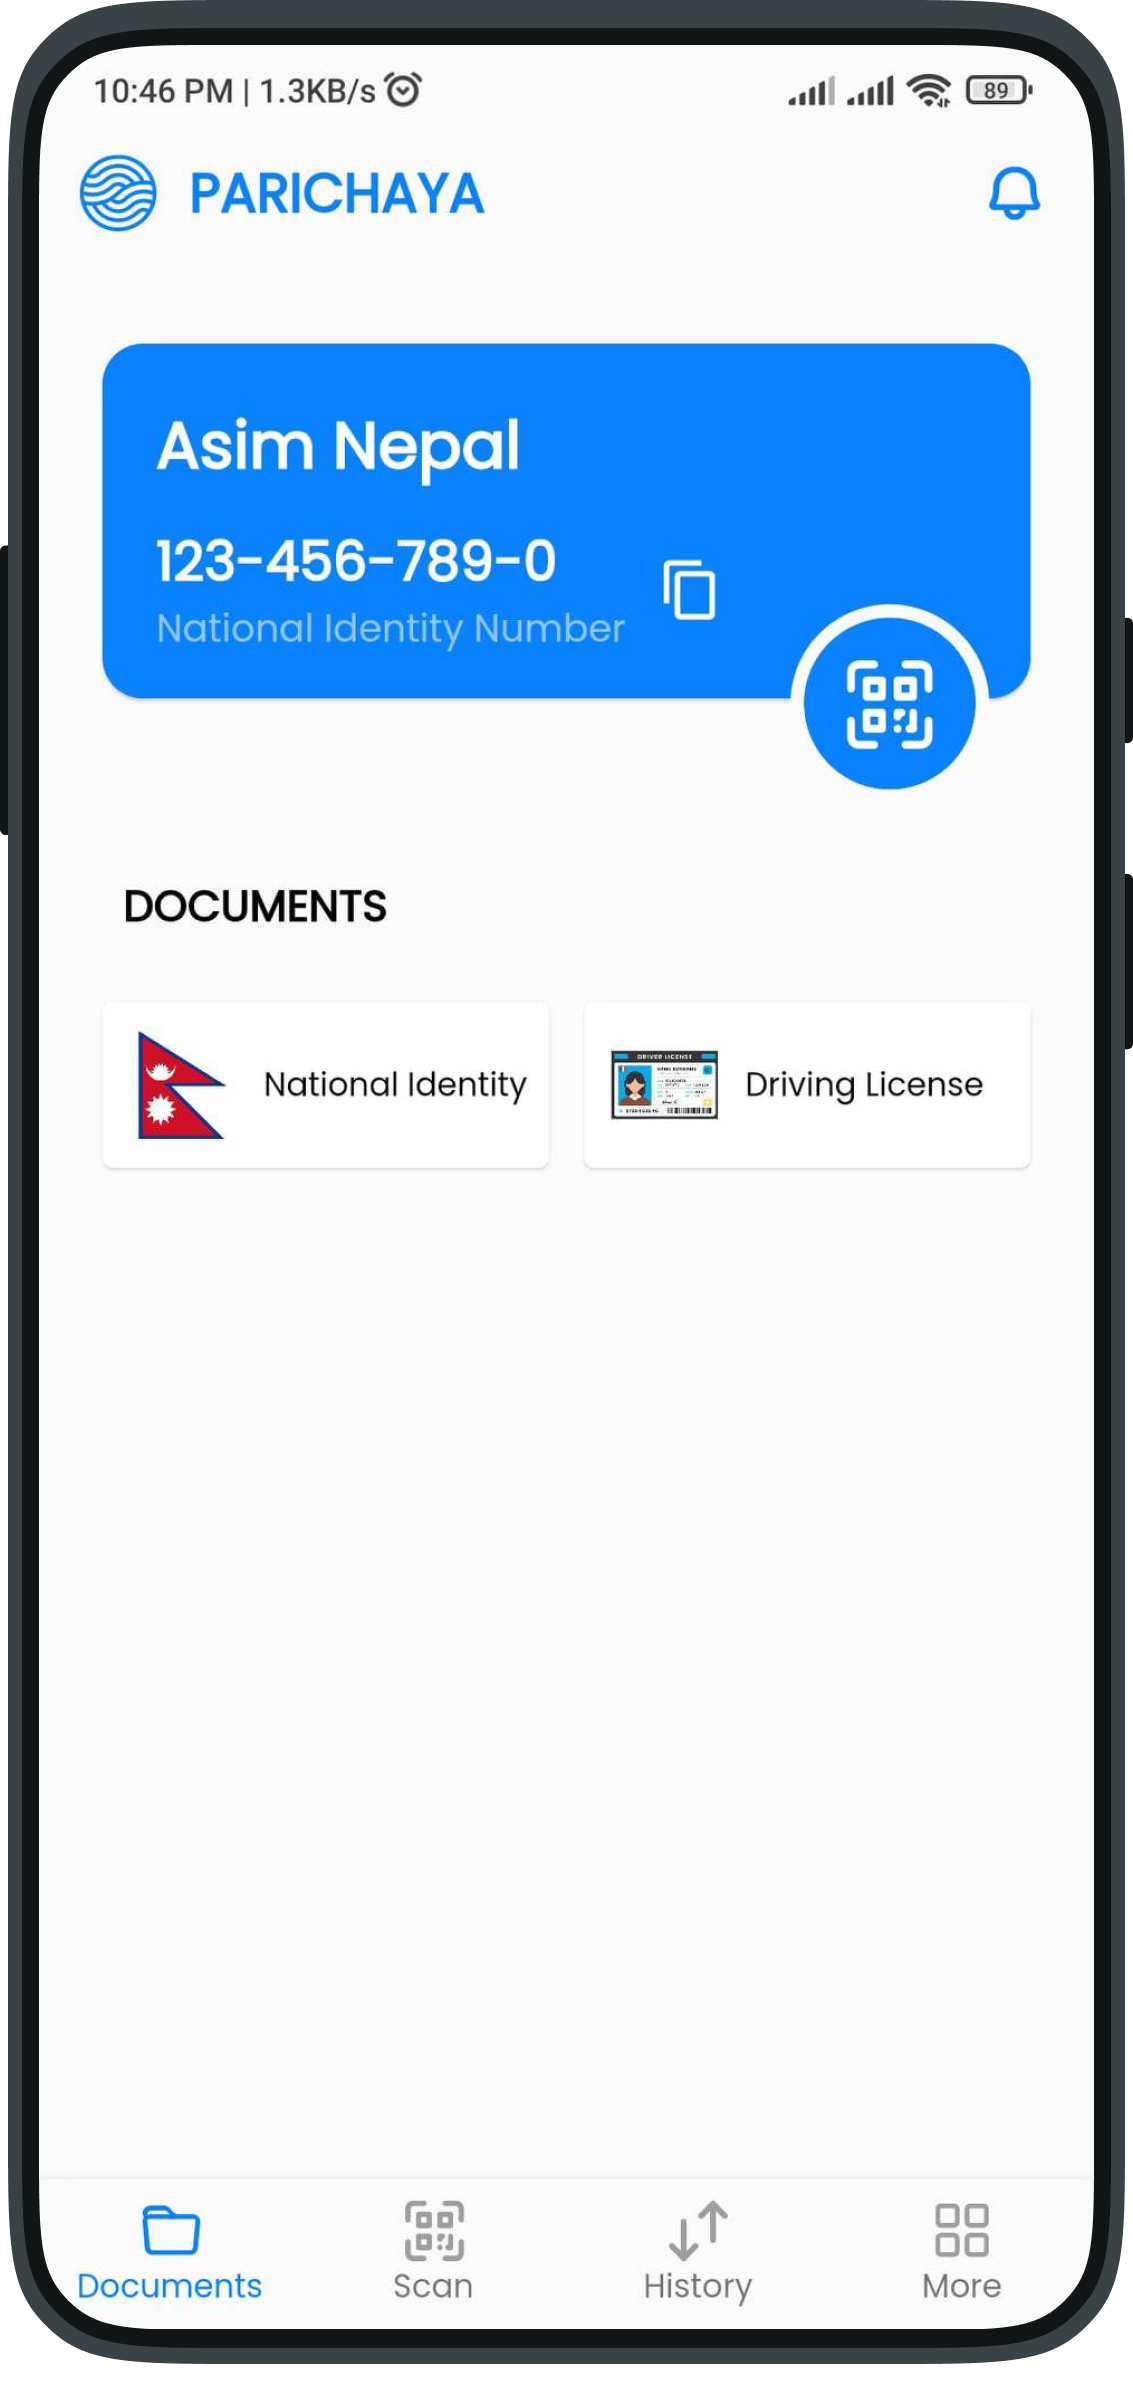
\includegraphics[width=0.6\linewidth]{images/results/mobile/Home.png}
        \caption[Document List View]{Document List View}
        \label{fig:Home.png}
        \end{figure} 
    \begin{figure}[H]
        \centering
        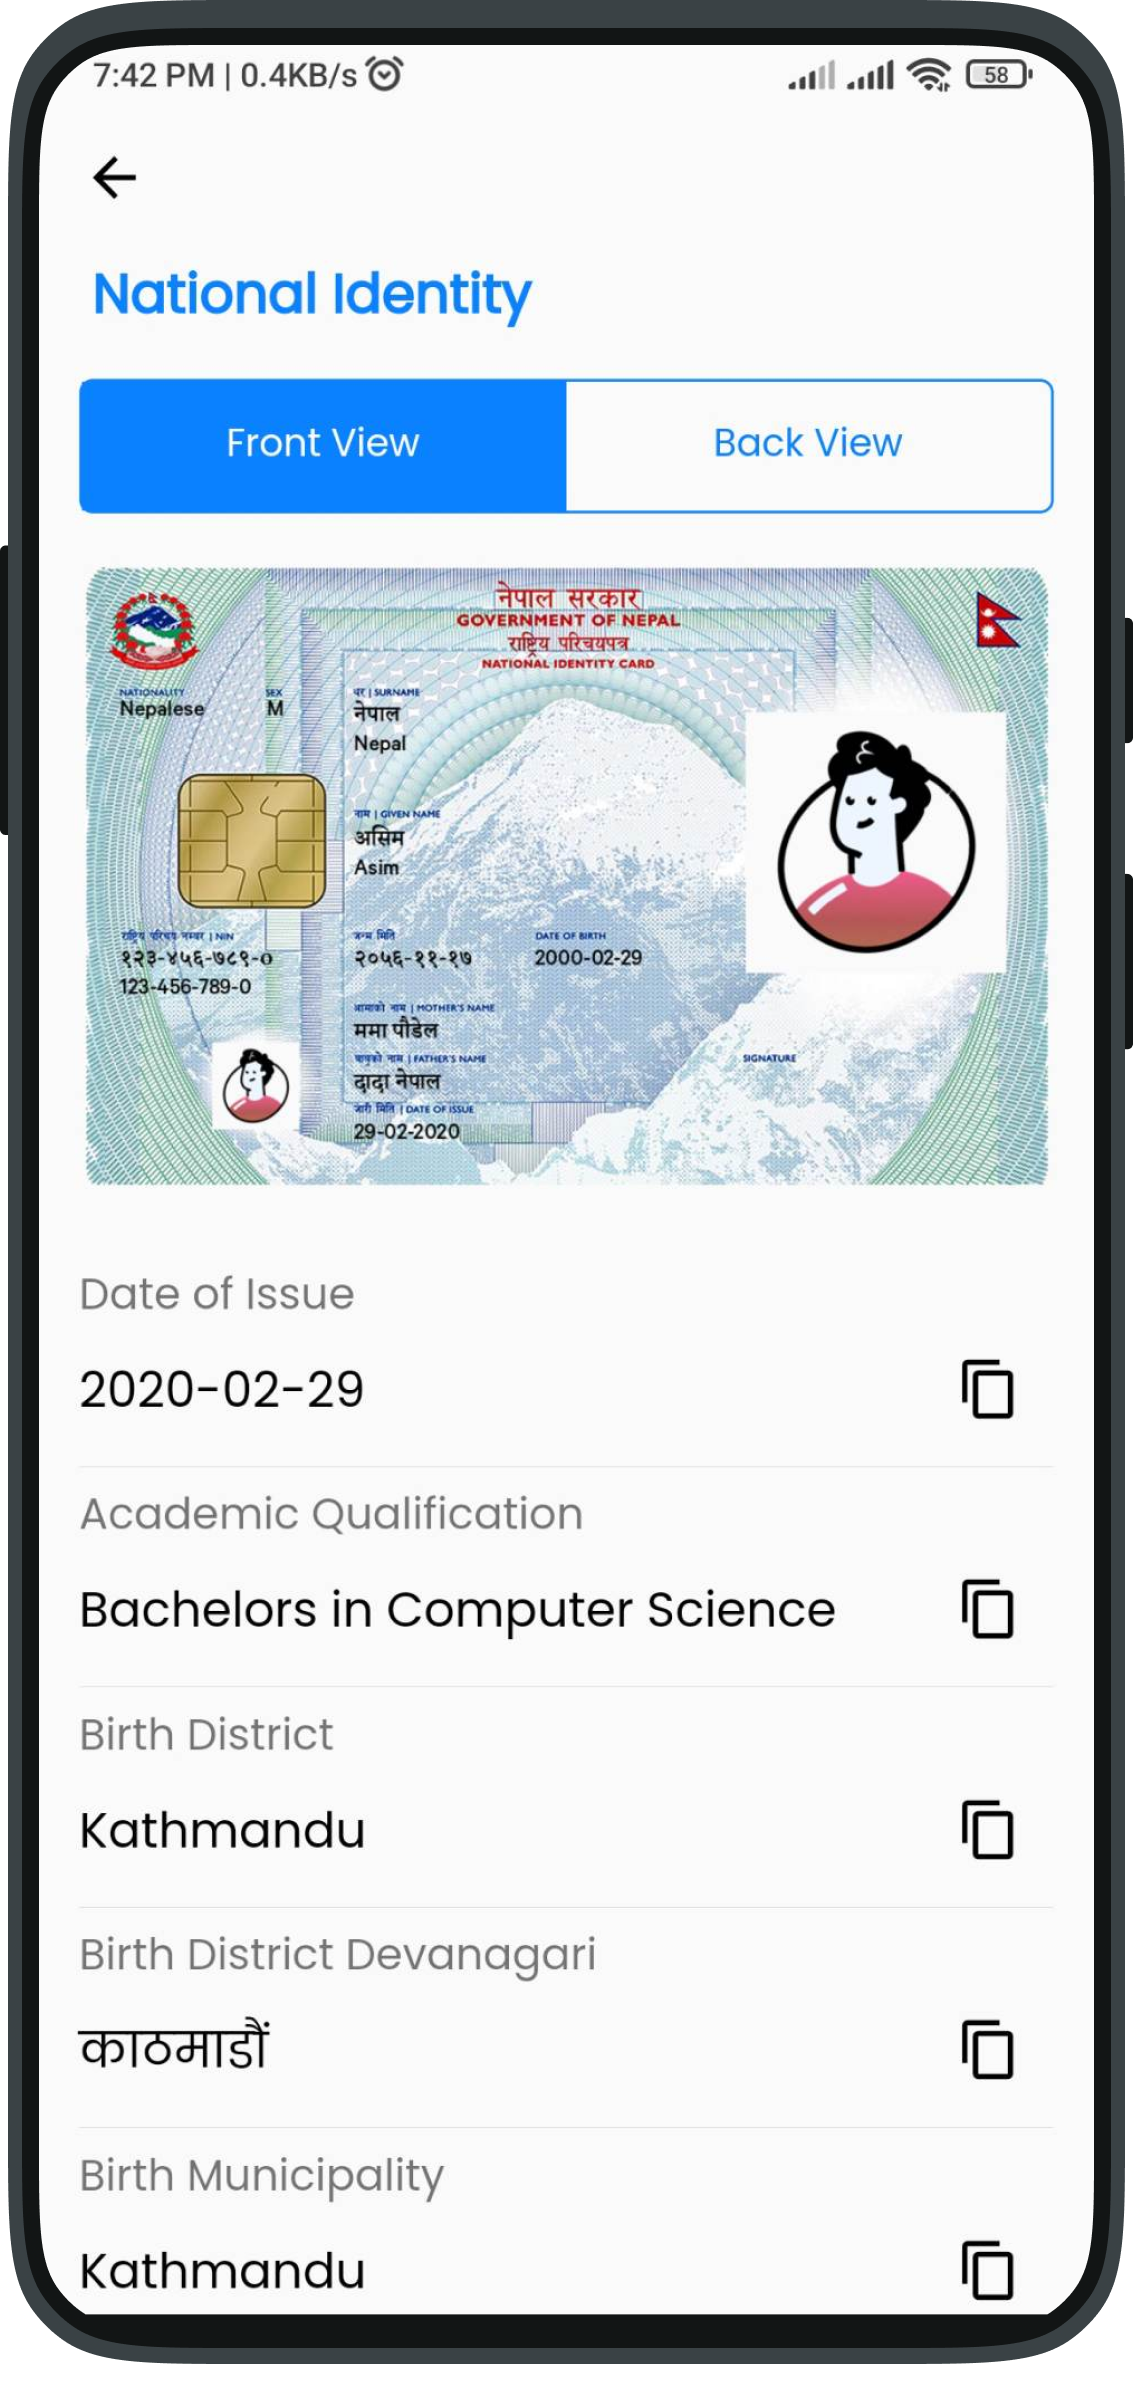
\includegraphics[width=0.6\linewidth]{images/results/mobile/NationalIdentity.png}
        \caption[Document Detail View ]{Document Detail View}
        \label{fig:NationalIdentity.png}
        \end{figure}     
\end{multicols}

\textbf{Document Share}\\
        User can share their driving license information to the traffic officer. Traffic police can either view it in user's phone or they can scan a QR code which contains driving license information.
        \begin{multicols}{2}
           \begin{figure}[H]
        \centering
        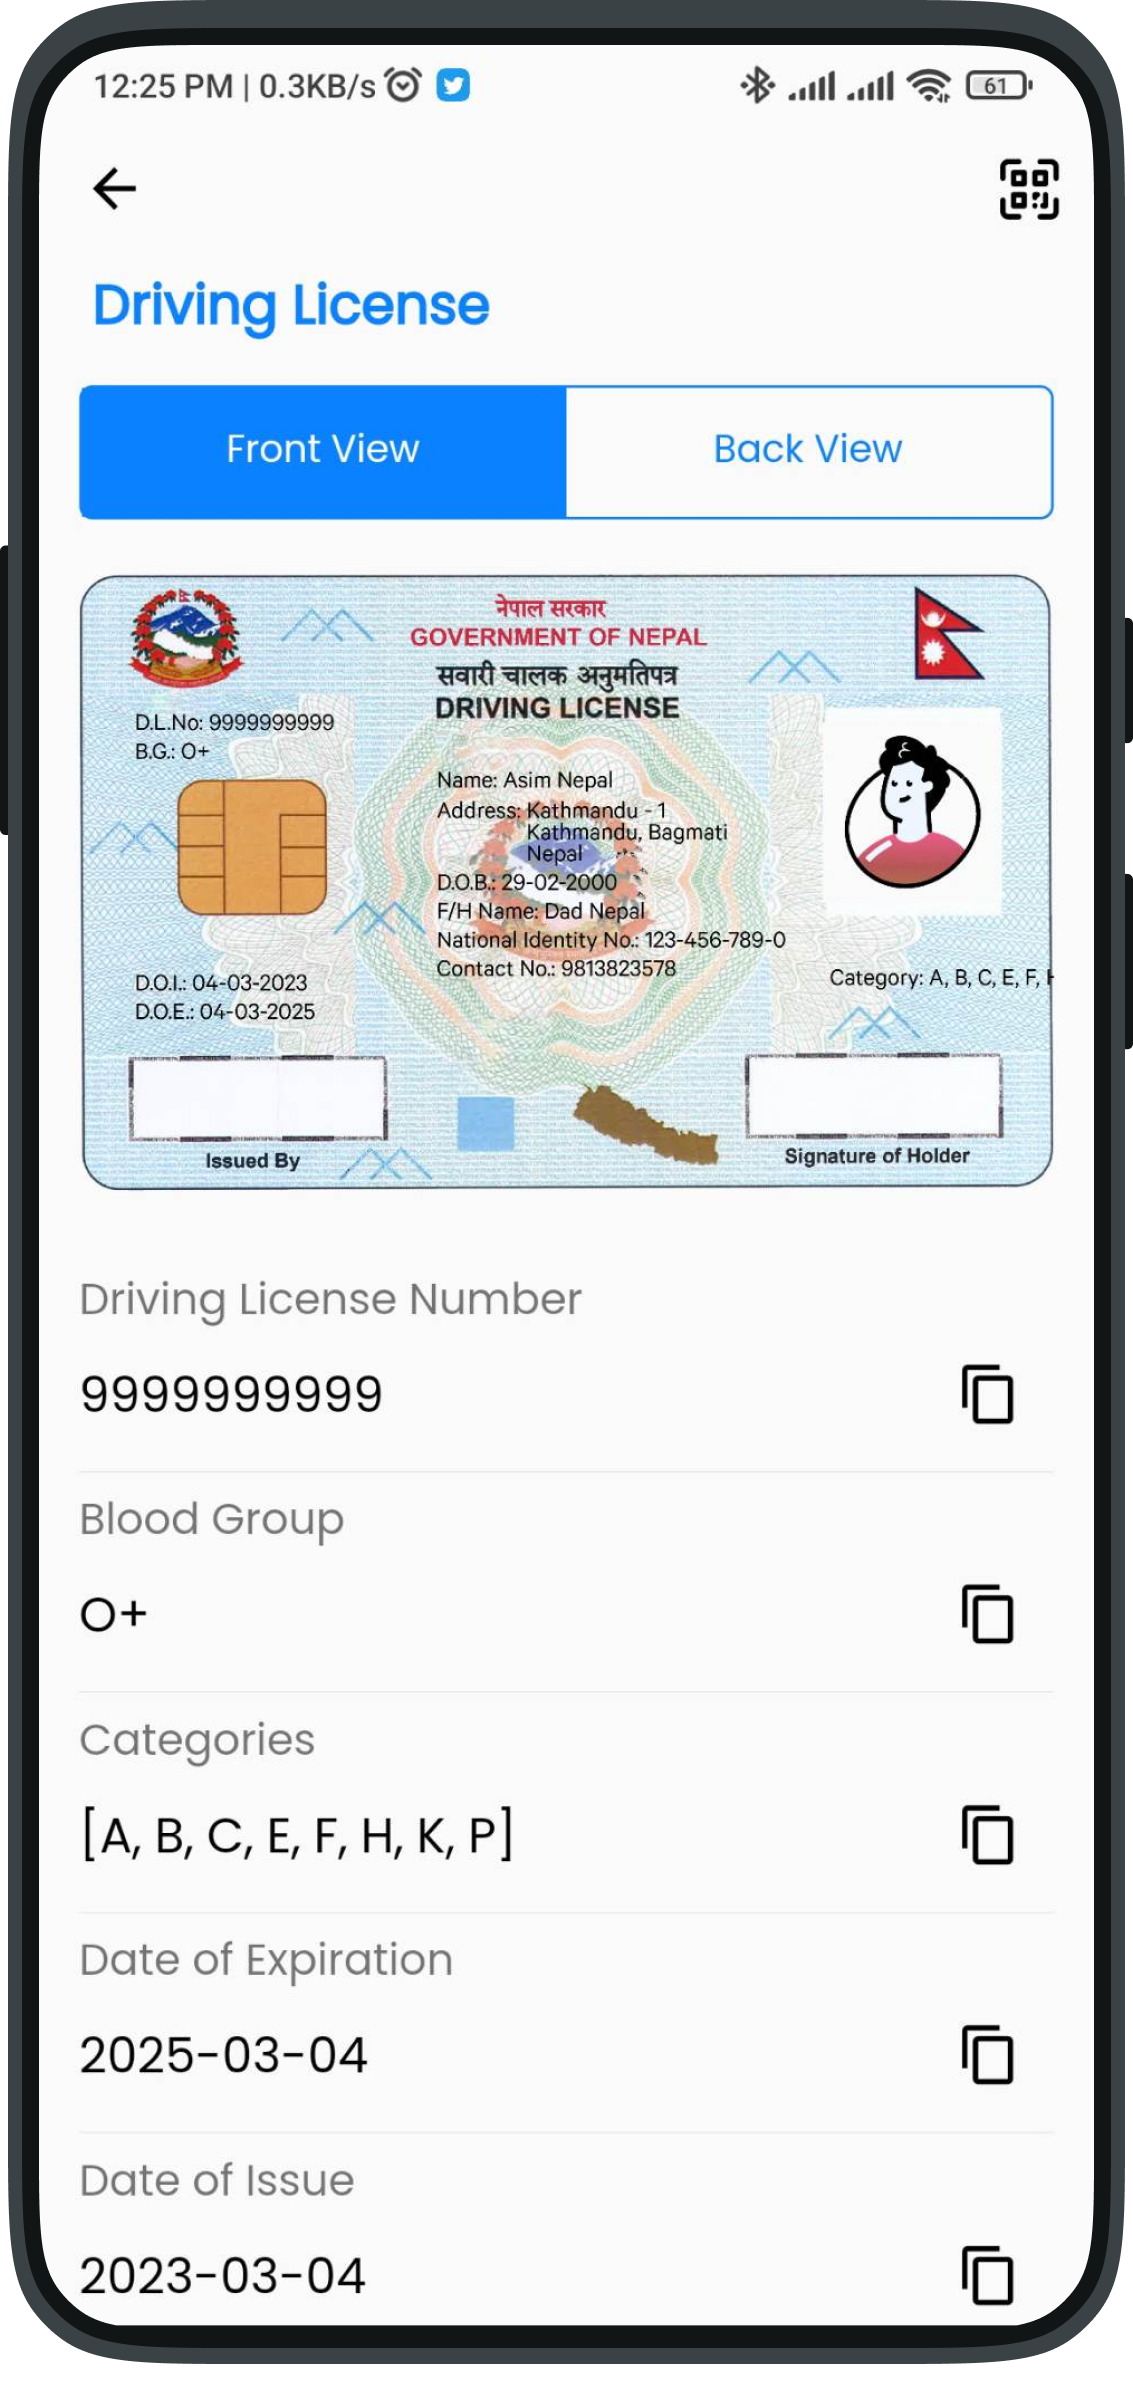
\includegraphics[width=0.6\linewidth]{images/results/mobile/DrivingLicense.png}
        \caption[Driving License ]{Driving License}
        \label{fig:DrivingLicense.png}
        \end{figure} 
        \begin{figure}[H]
        \centering
        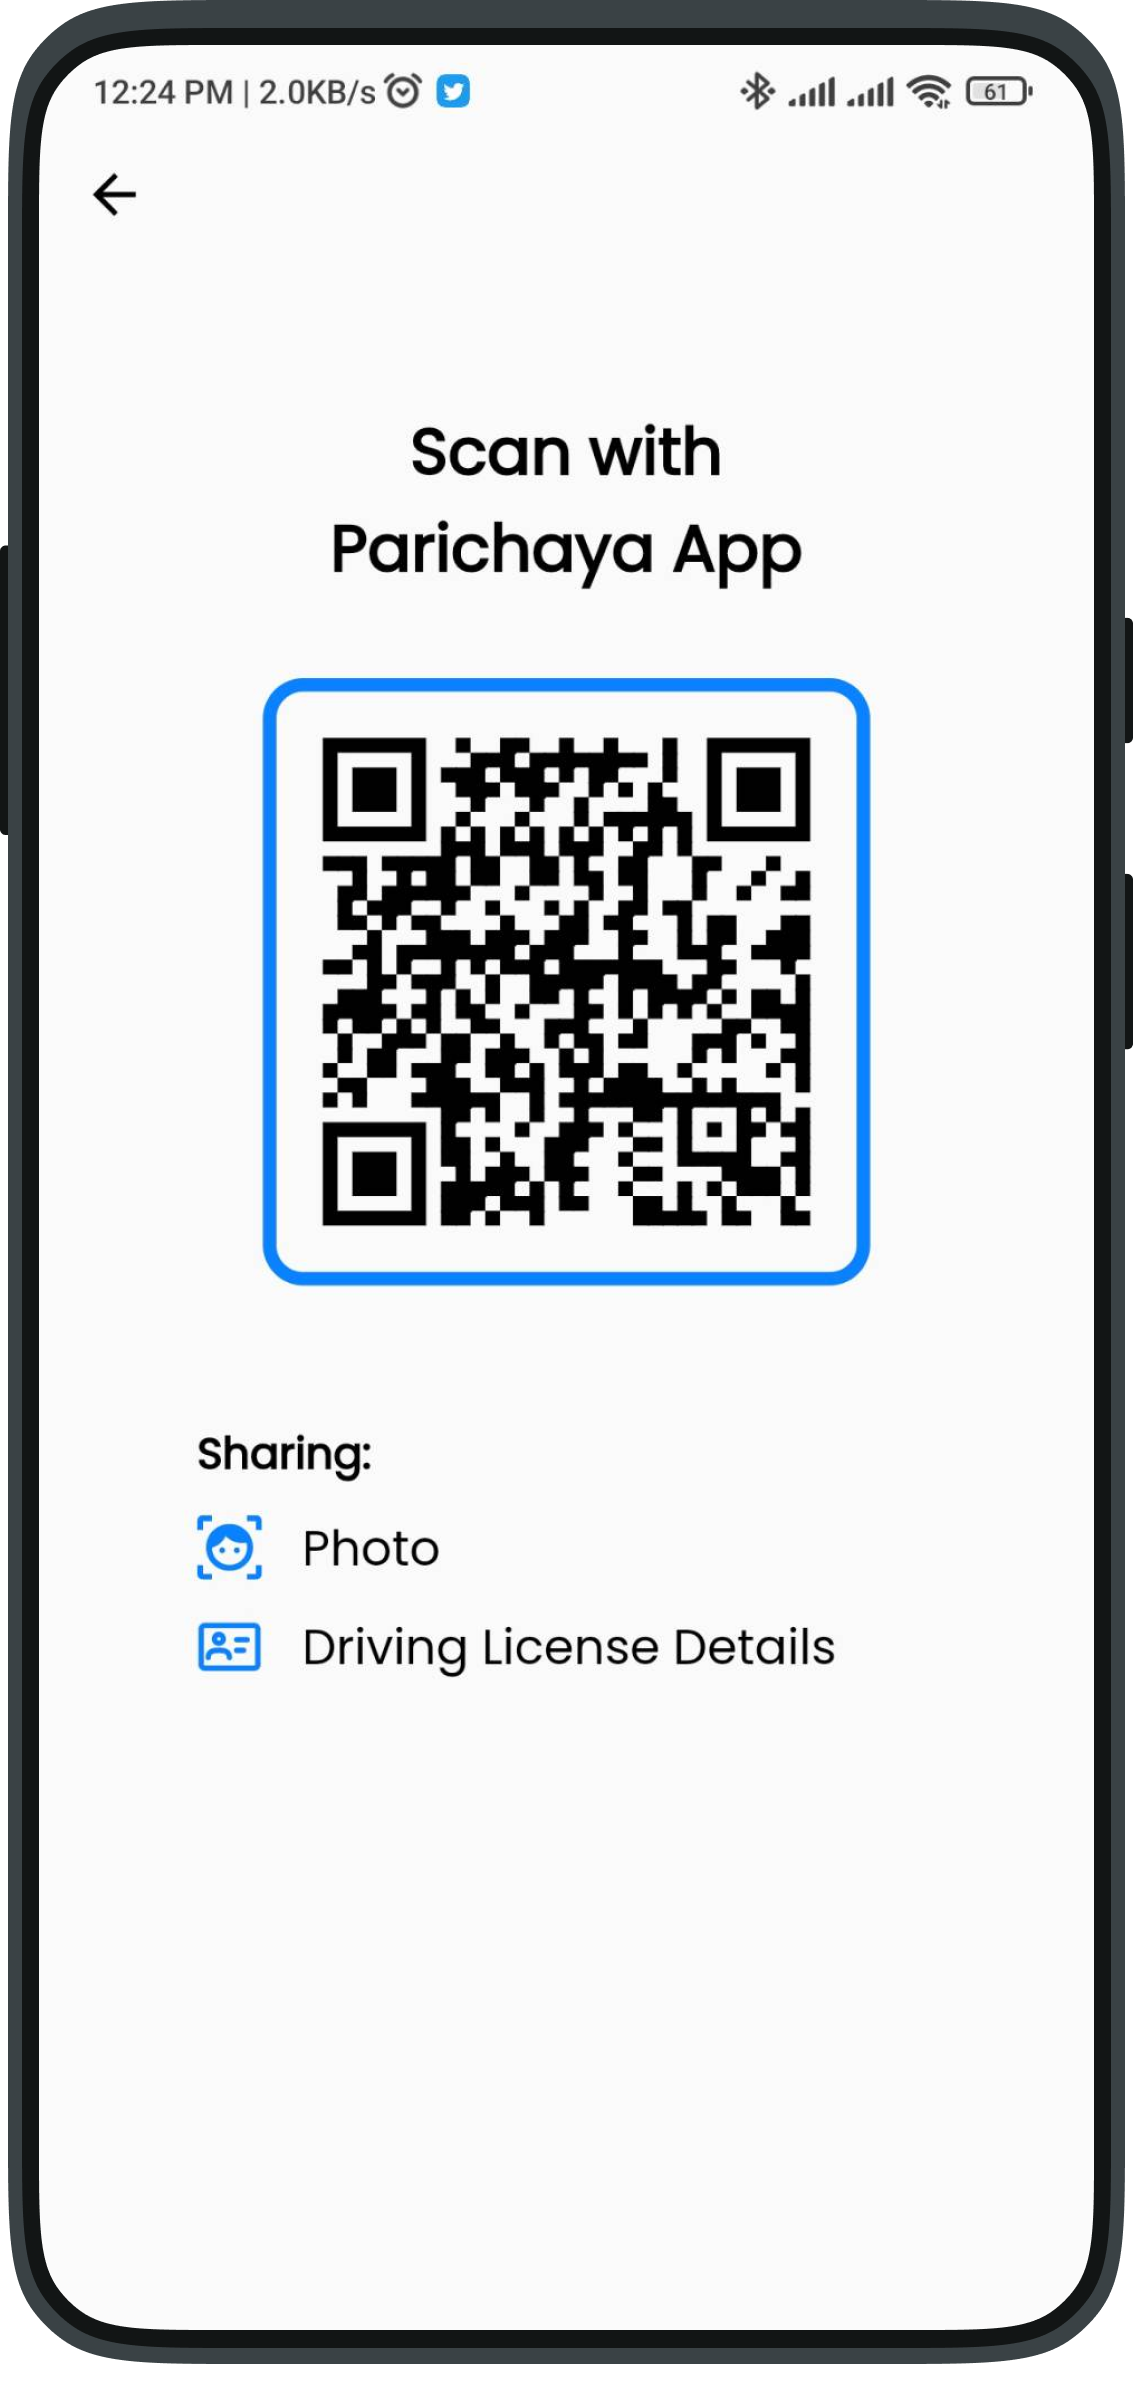
\includegraphics[width=0.6\linewidth]{images/results/mobile/DrivingLicenseQR.png}
        \caption[Share Driving License]{Share Driving License}
        \label{fig:DrivingLicenseQR.png}
        \end{figure} 
        \end{multicols}

        \textbf{Scan QR}\\
        The app contains a QR scanner which can be used to scan QR codes generated by the system to view the shared details of other users, or to share details to third party applications.
        \begin{figure}[H]
        \centering
        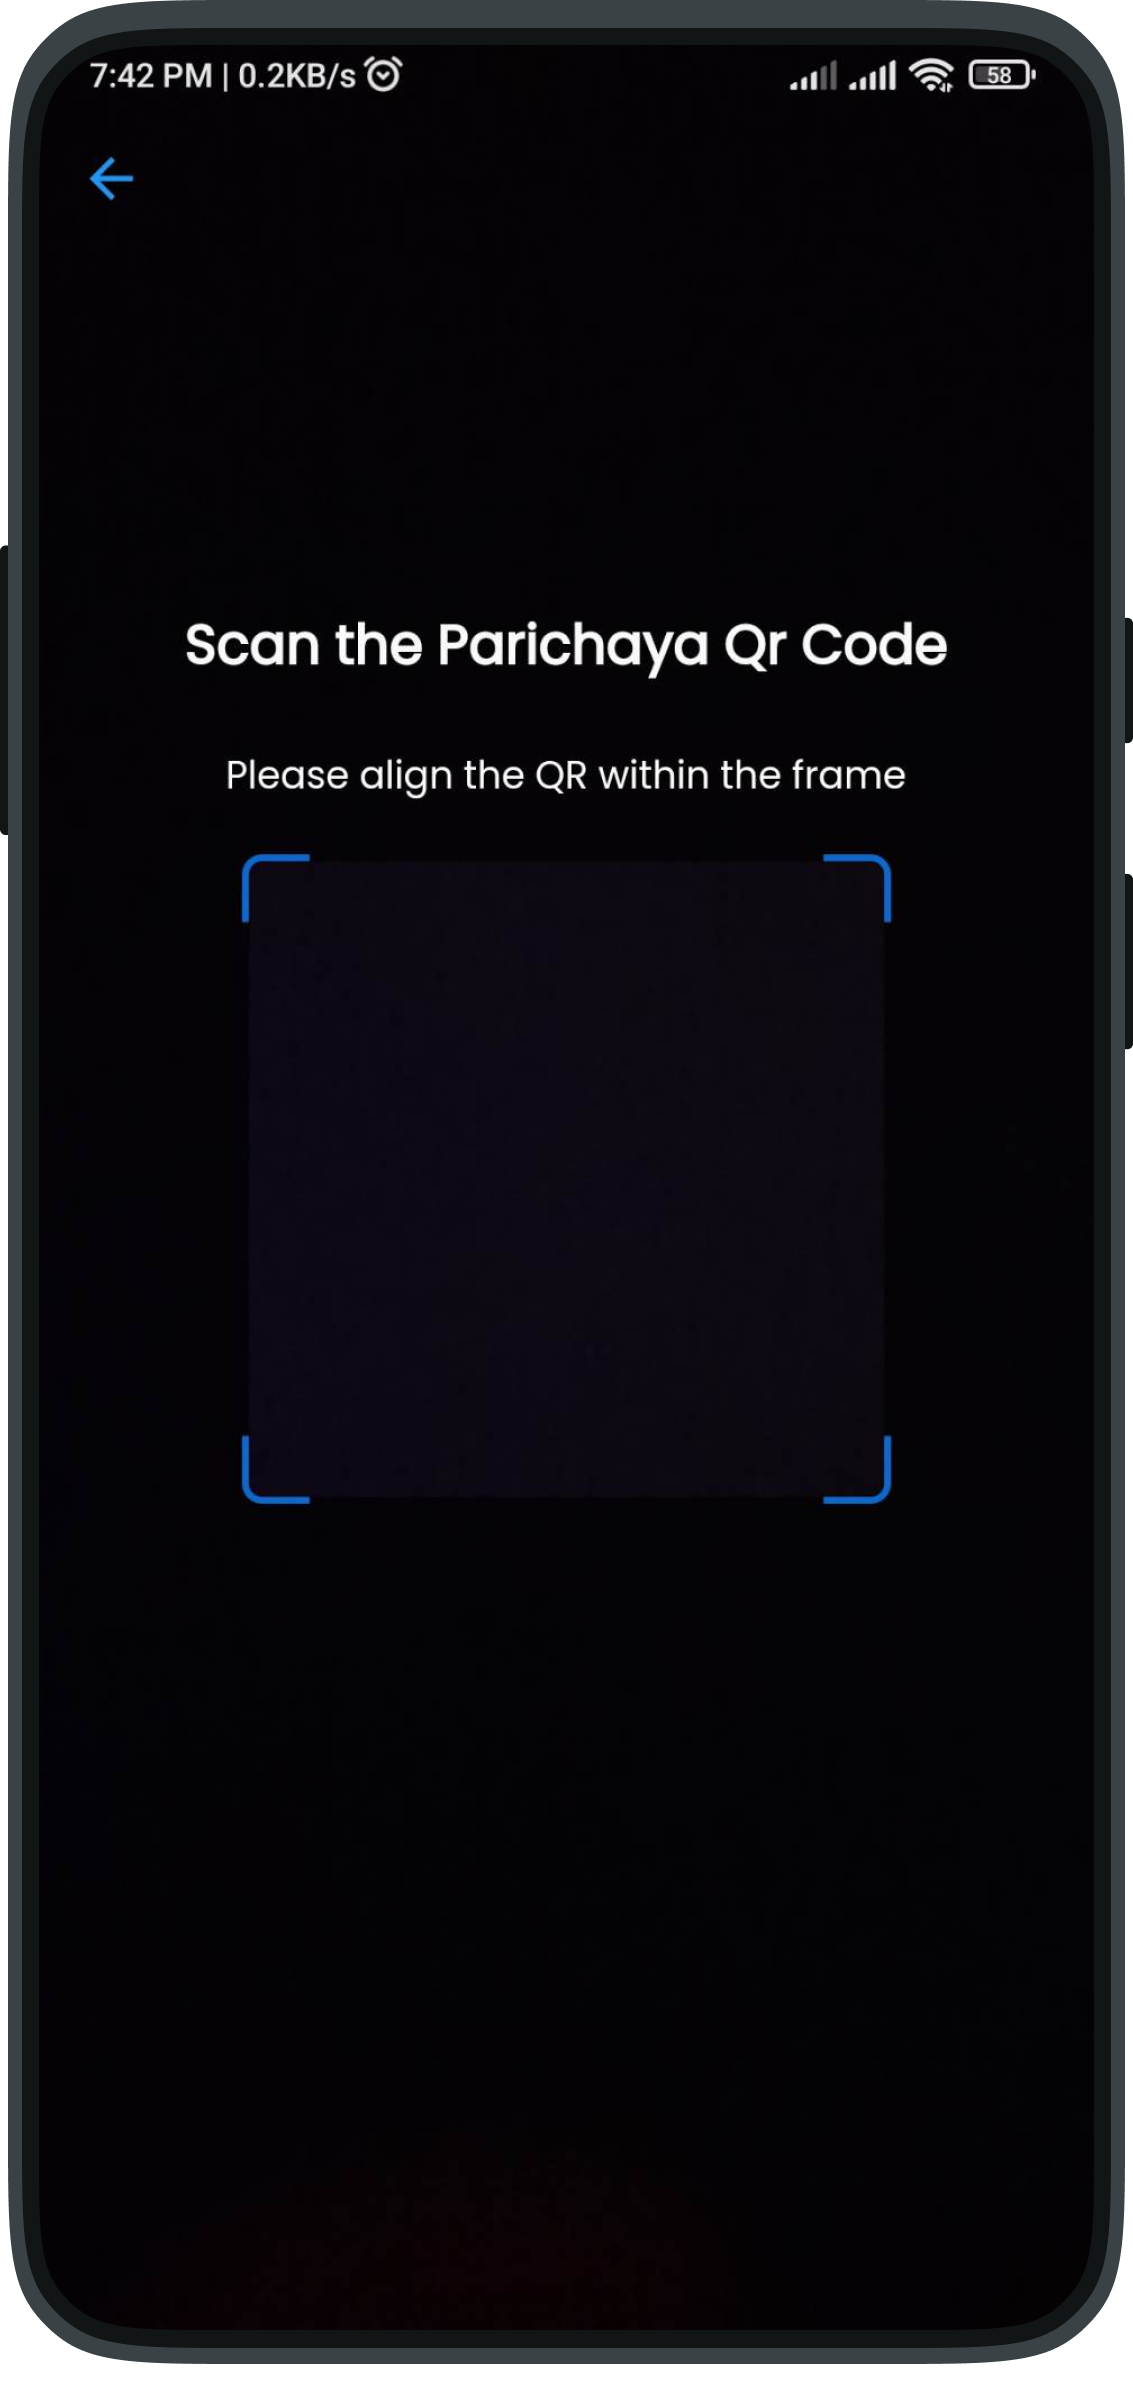
\includegraphics[width=0.3\linewidth]{images/results/mobile/QRScan.png}
        \caption[Scan QR Screen]{Scan QR Screen}
        \label{fig:QRScan.png}
        \end{figure}  
        
        \textbf{Age Verification}\\
        Verify Age is a basic feature for users to view their verified age. The user may share their age or driving license by generating the qr code with a touch of a button and the users who want to obtain this information can scan the qr code using Parichaya app. The user who shared the information will get real time update on who is viewing their data.
        \begin{multicols}{3}
            \begin{figure}[H]
            \centering
            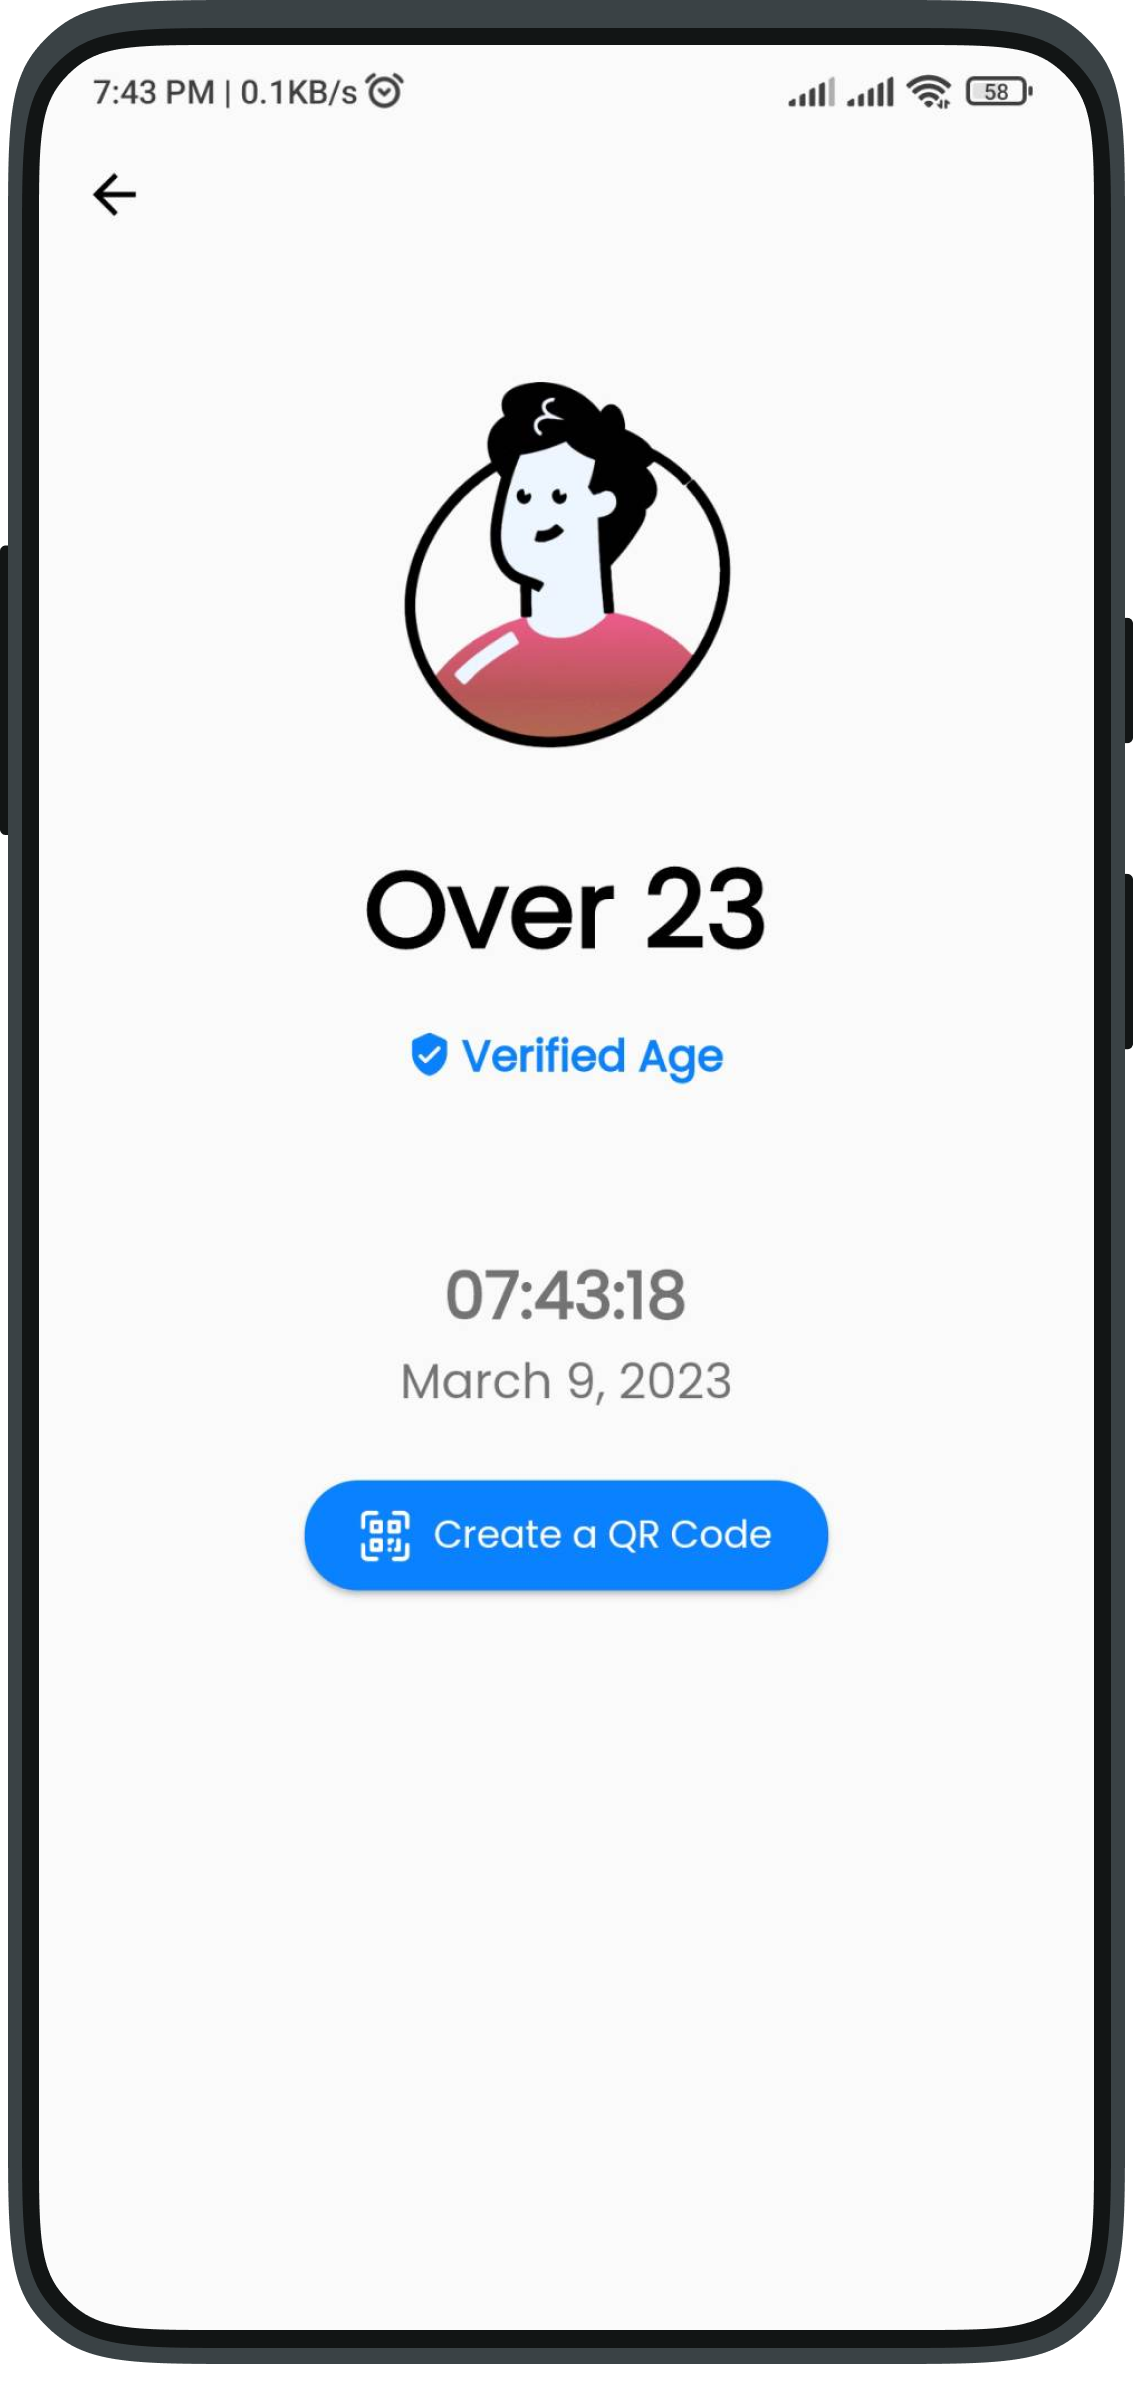
\includegraphics[width=0.8\linewidth]{images/results/mobile/VerifyAge.png}
            \caption[Verified Age]{Verified Age}
            \label{fig:VerifyAge.png}
            \end{figure}
              \begin{figure}[H]
            \centering
            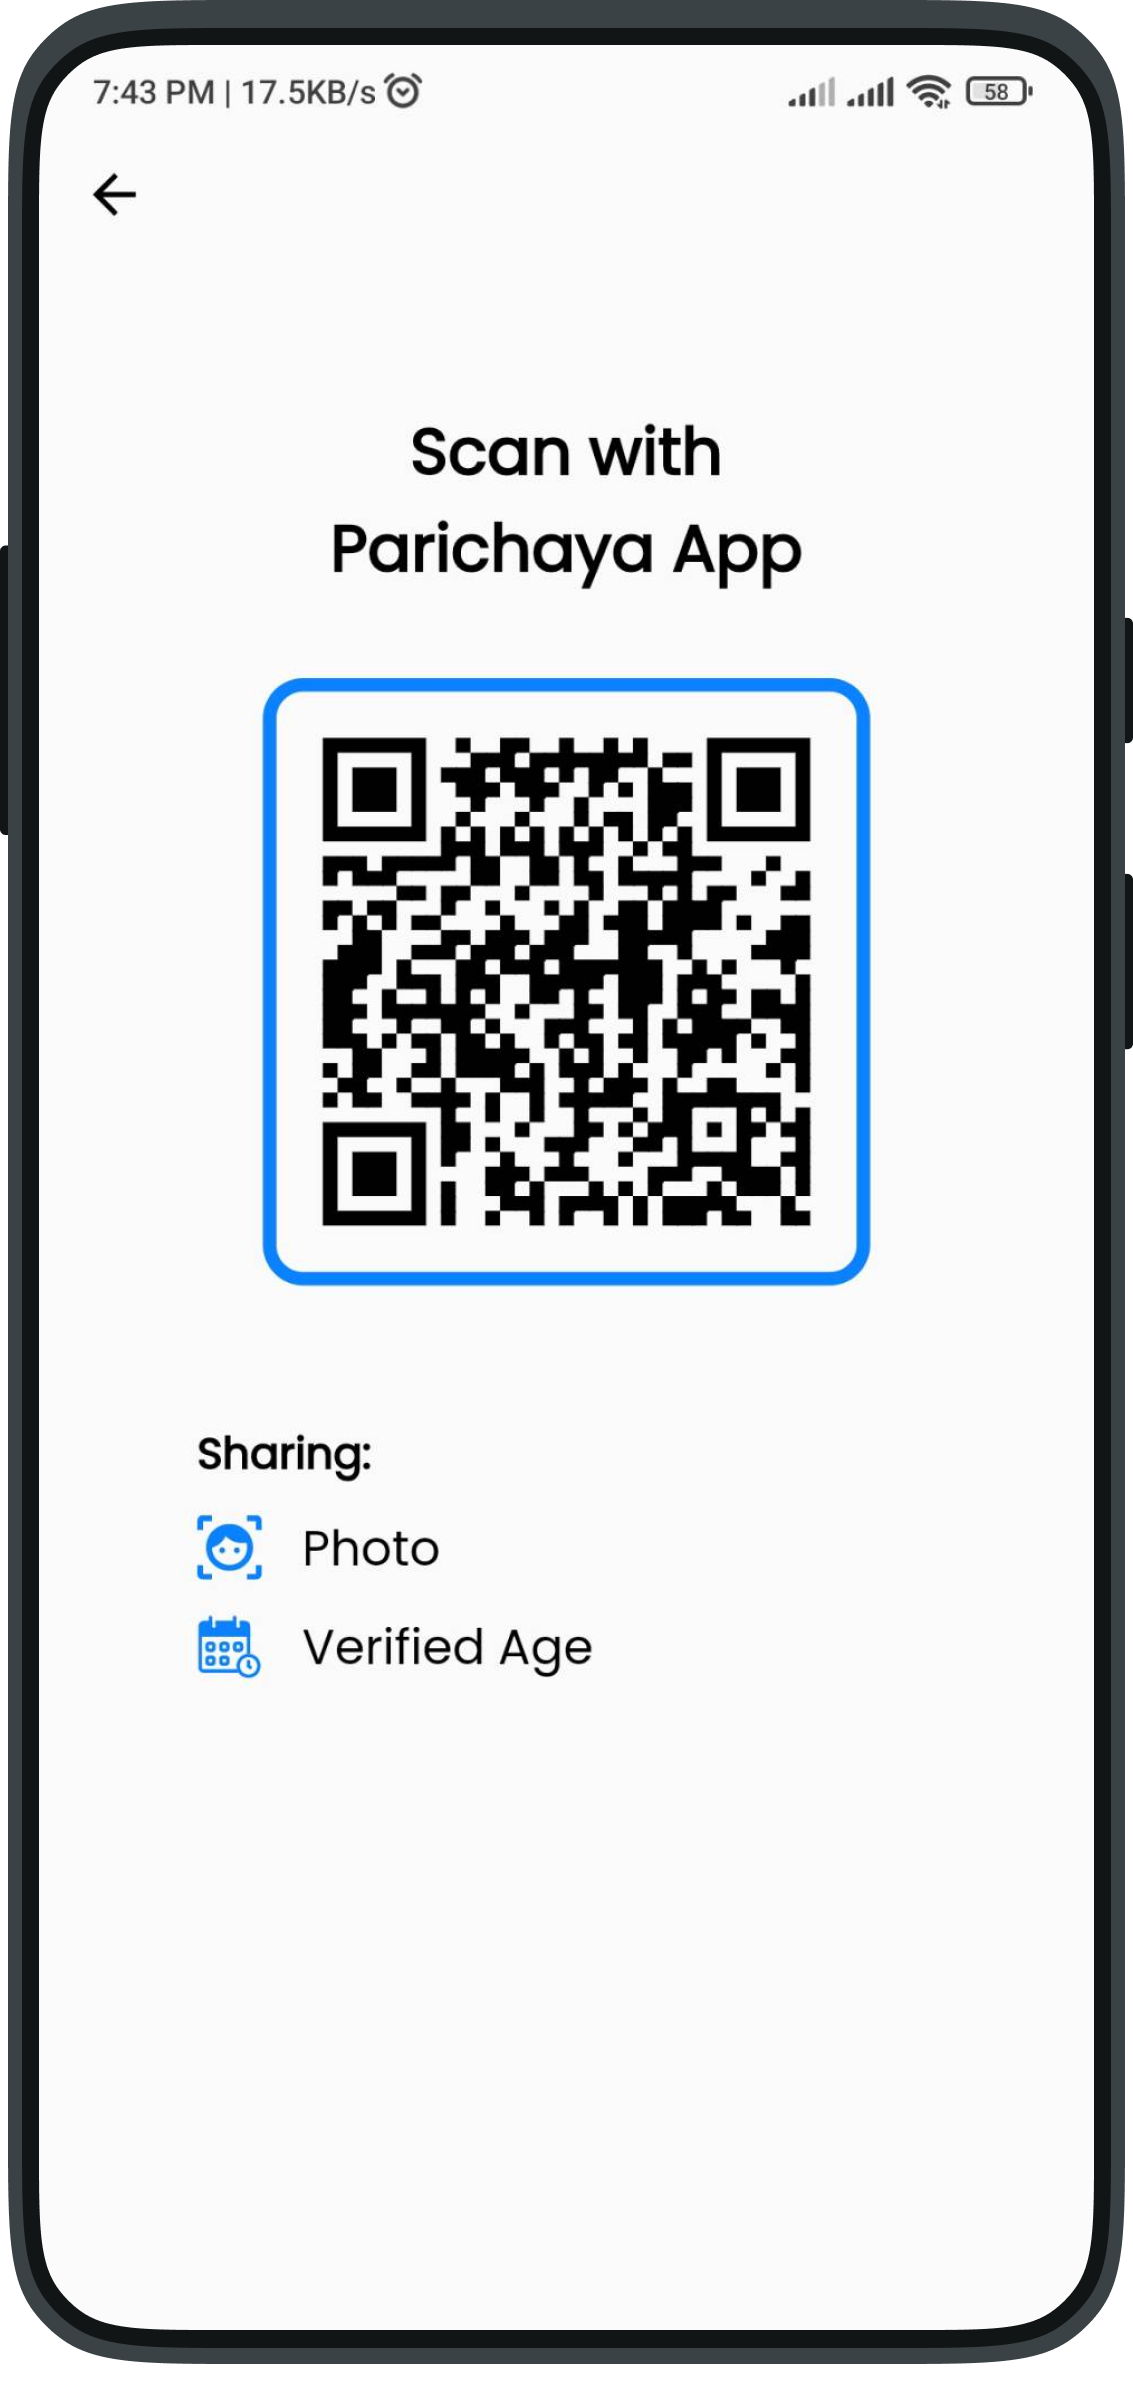
\includegraphics[width=0.8\linewidth]{images/results/mobile/VerifyAgeQR.png}
            \caption[Share Age]{Share Age}
            \label{fig:VerifyAgeQR.png}
            \end{figure}
              \begin{figure}[H]
            \centering
            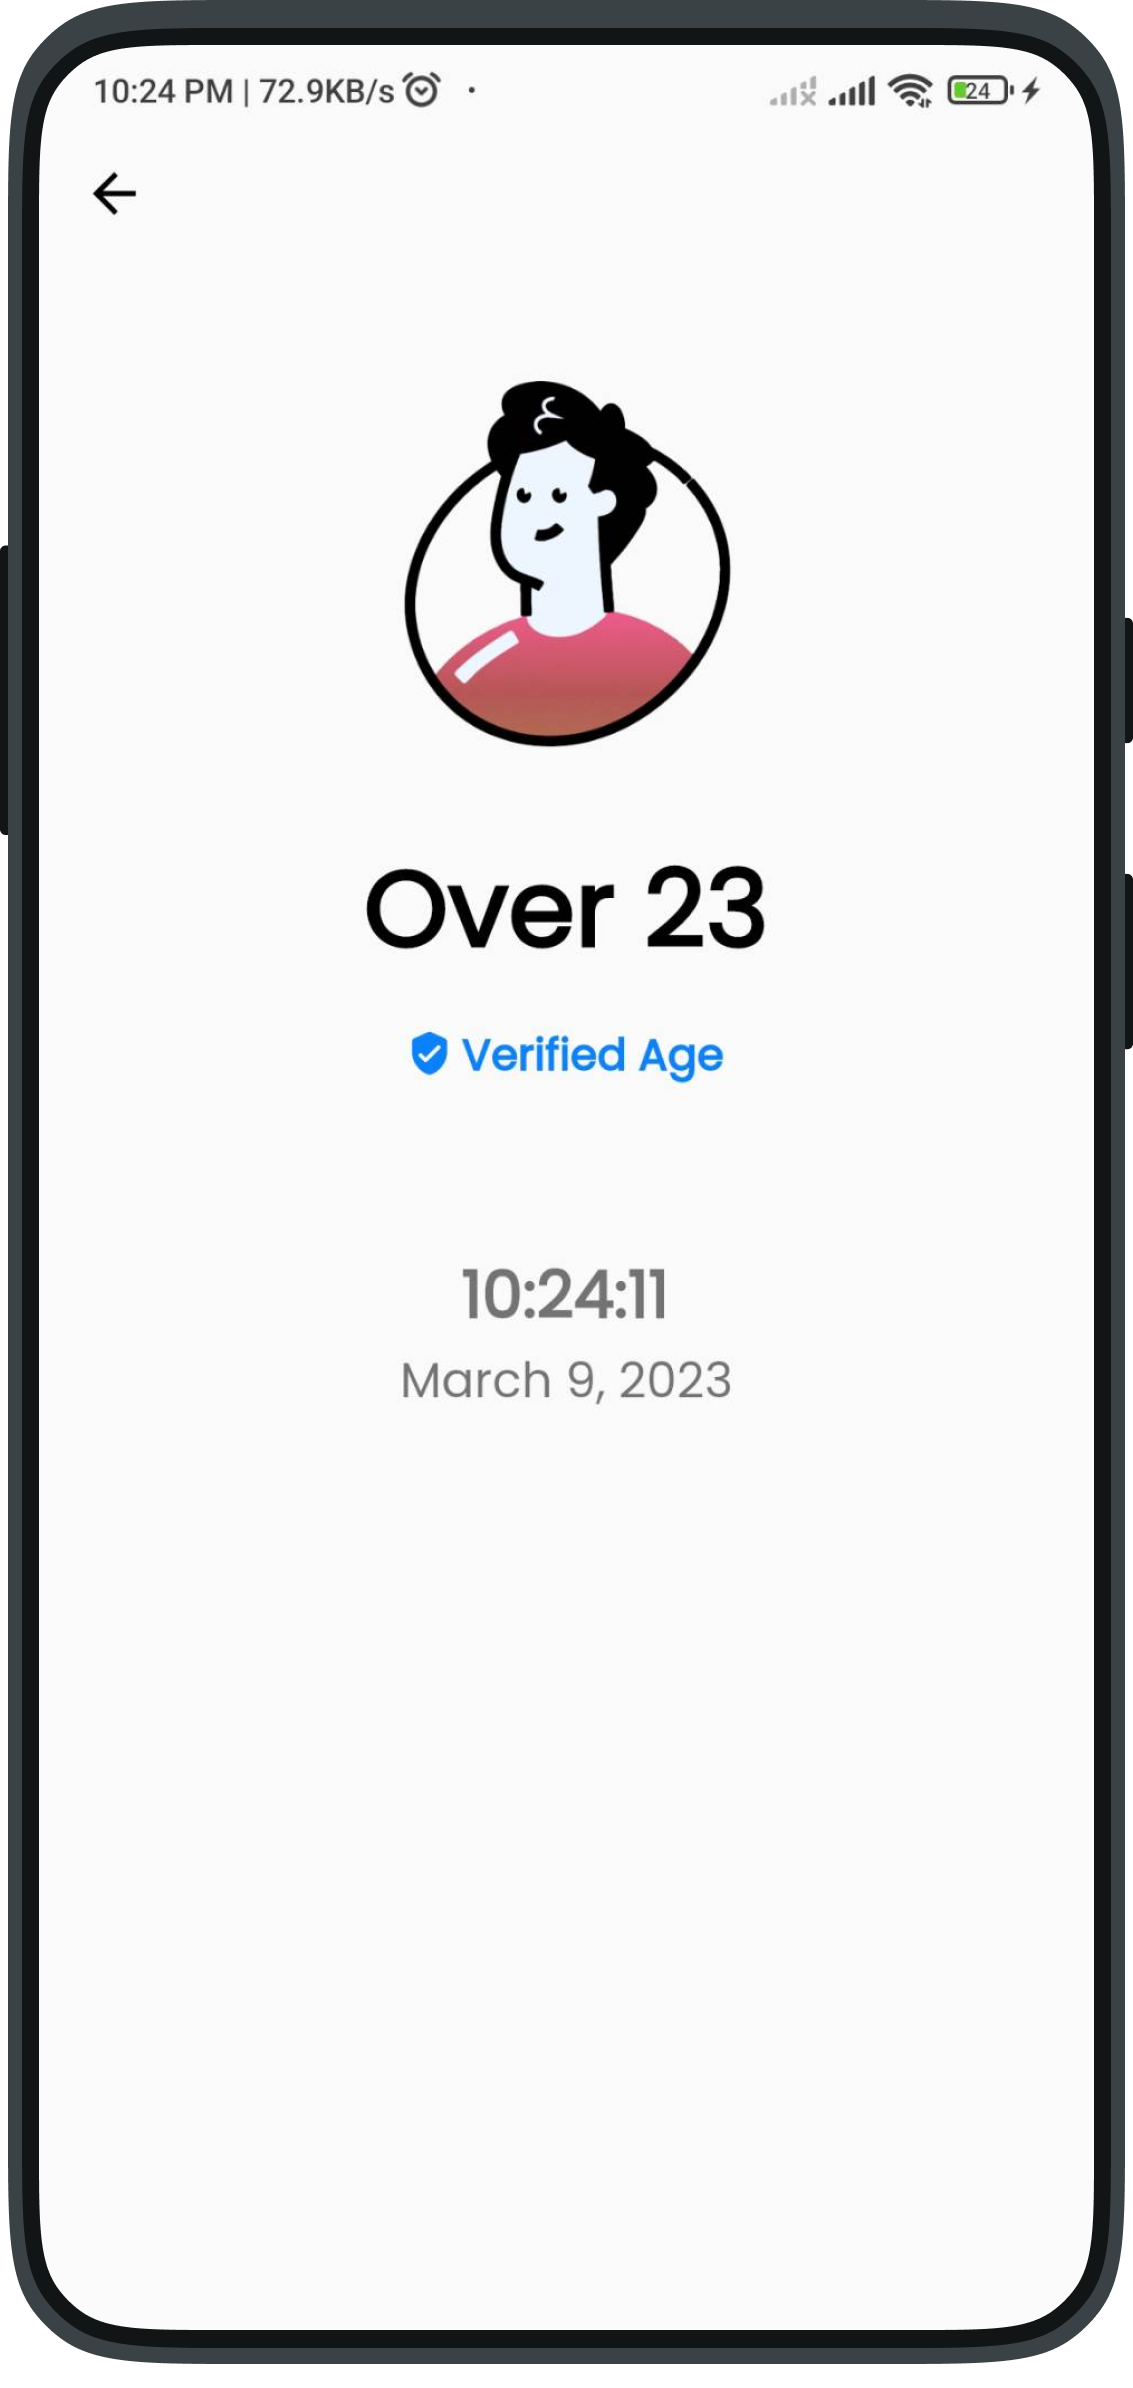
\includegraphics[width=0.8\linewidth]{images/results/mobile/VerifiedAgeShared.png}
            \caption[Shared Age]{Shared Age}
            \label{fig:VerifiedAgeShared.png}
            \end{figure}
            
        \end{multicols}
        \textbf{Document Share to Third Party Application}\\
        The user can share their information as required by third party applications. Here, the user scans the qr code generated by the third party (like banks) and will view all the information required to share. The user then may approve or deny the request.
         \begin{figure}[H]
            \centering
            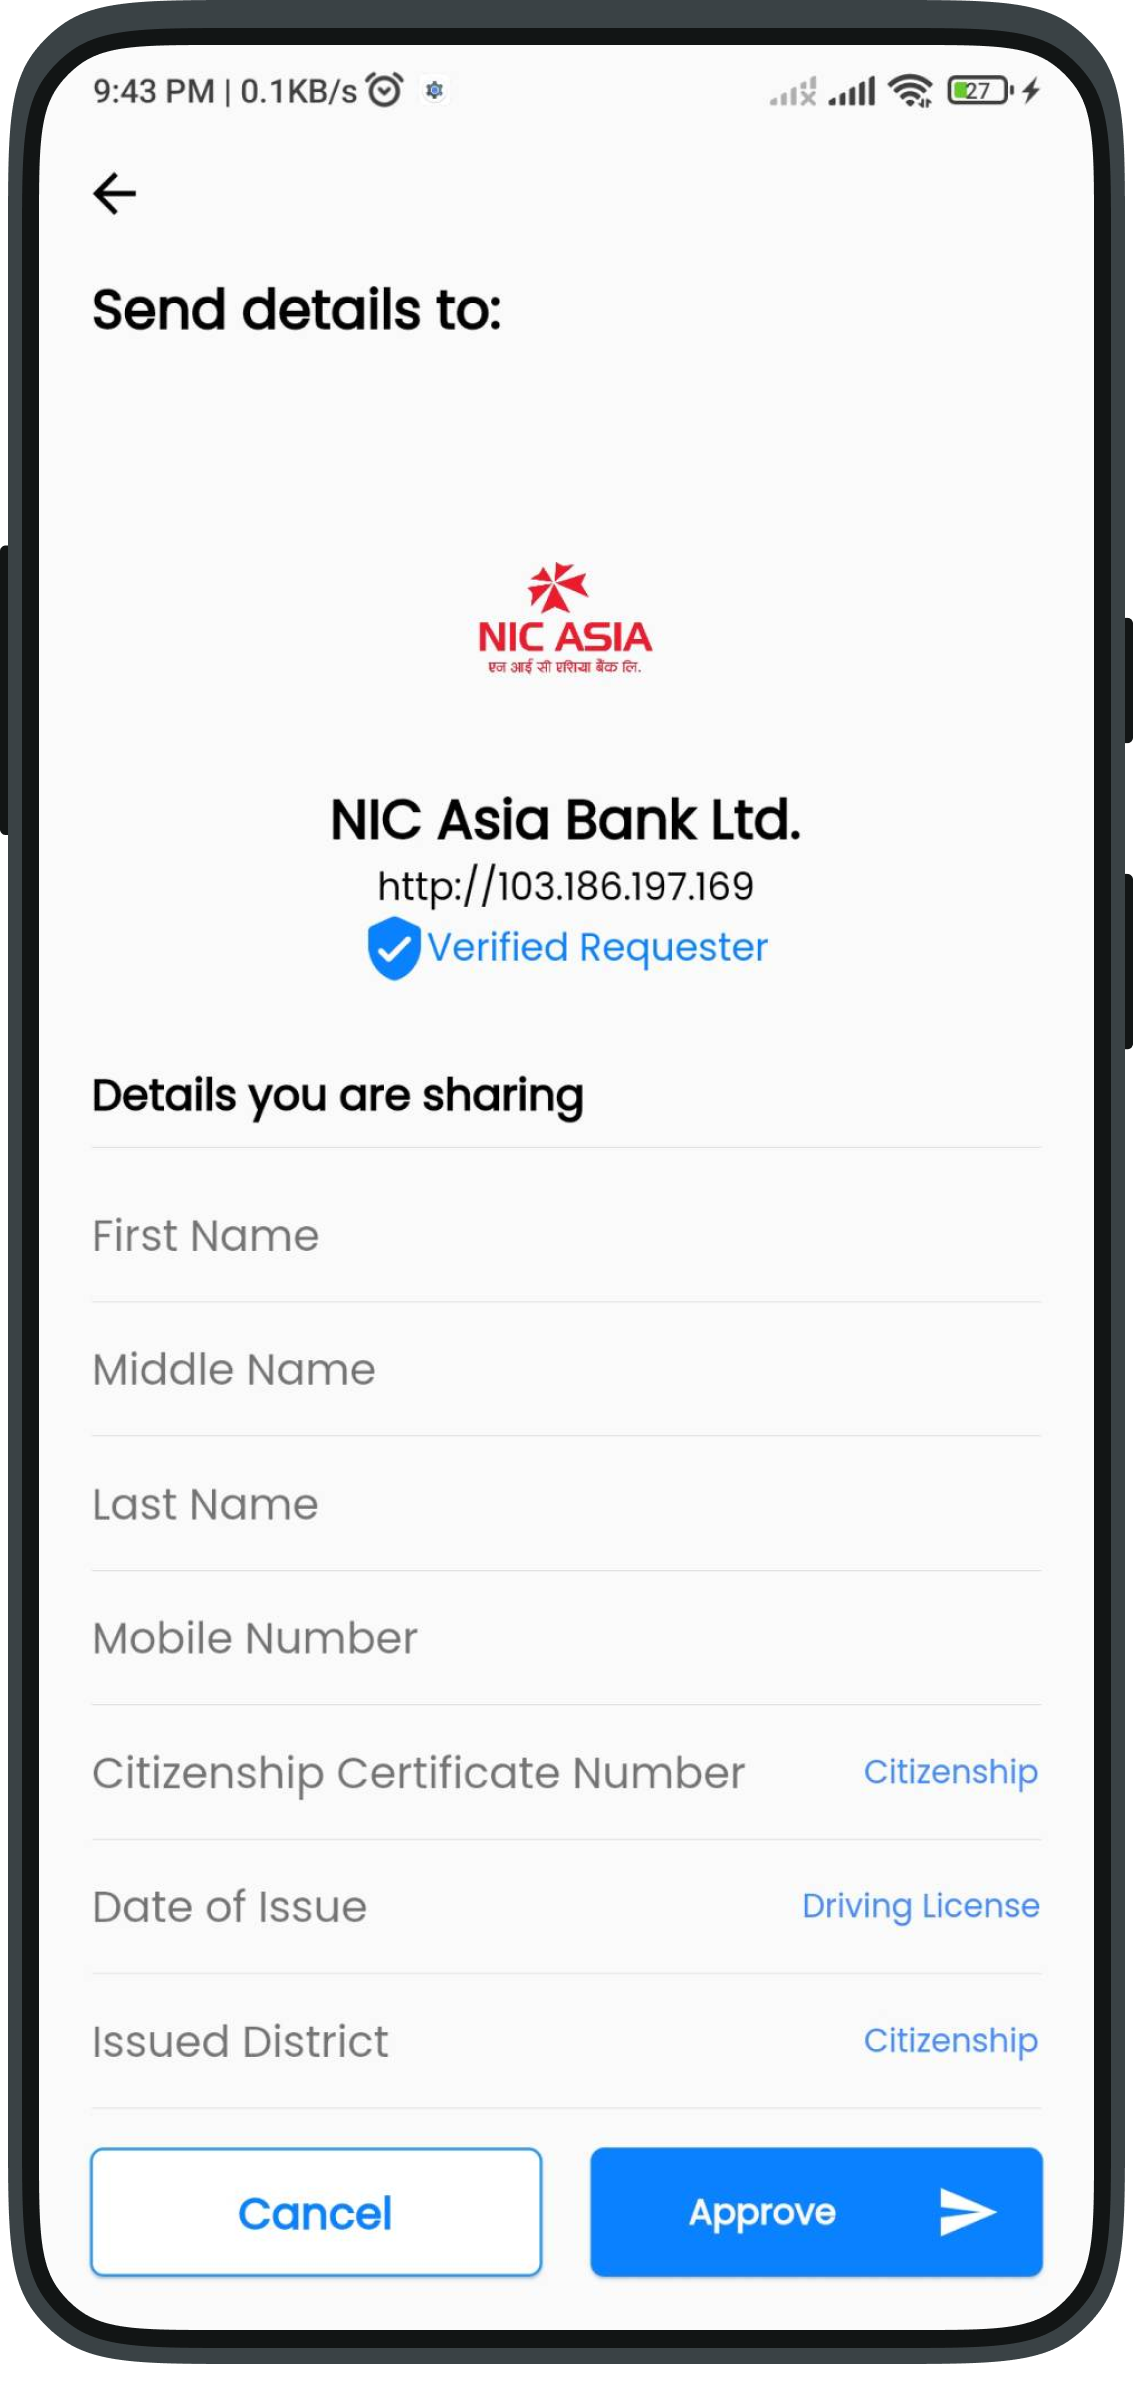
\includegraphics[width=0.3\linewidth]{images/results/mobile/DataAccessRequest.png}
            \caption[Access Request Permission Screen]{Access Request Permission Screen}
            \label{fig:DataAccessRequest.png}
            \end{figure}
        \textbf{Activity History}\\
        All of the user's activities, such as, logging into the device, generating QR codes to share details, scanning QR codes to obtain details, and much more are recorded and can be viewed in the history page. All the Shared or obtained details can be viewed by clicking on any of the history tile.
        \newpage
        \begin{multicols}{2}
            \begin{figure}[H]
            \centering
            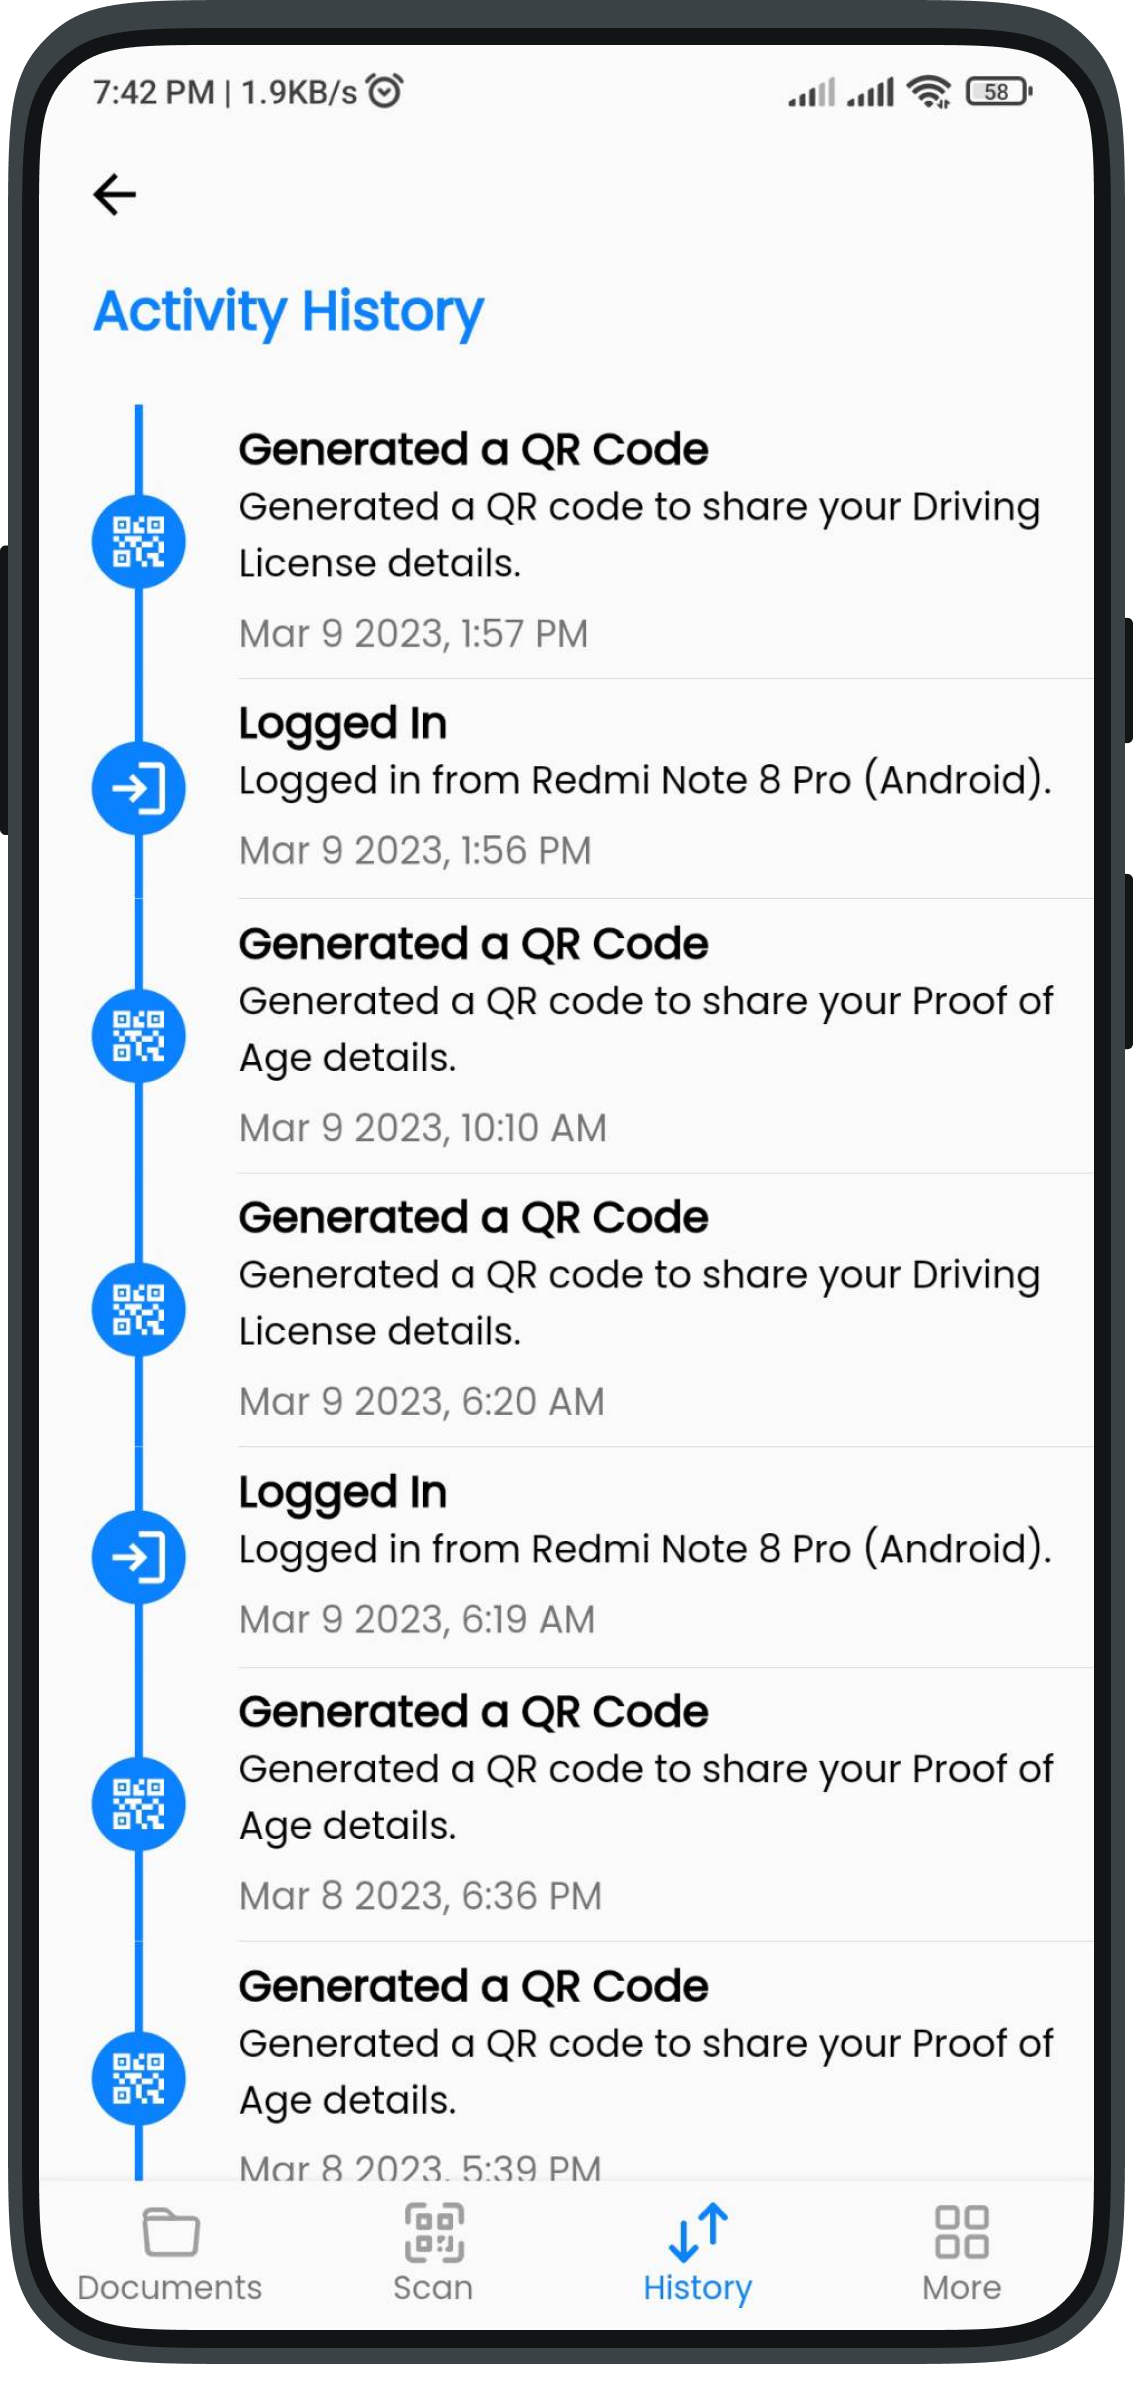
\includegraphics[width=0.6\linewidth]{images/results/mobile/History.png}
            \caption[Activity History Screen]{Activity History Screen}
            \label{fig:History.png}
            \end{figure} 

            \begin{figure}[H]
            \centering
            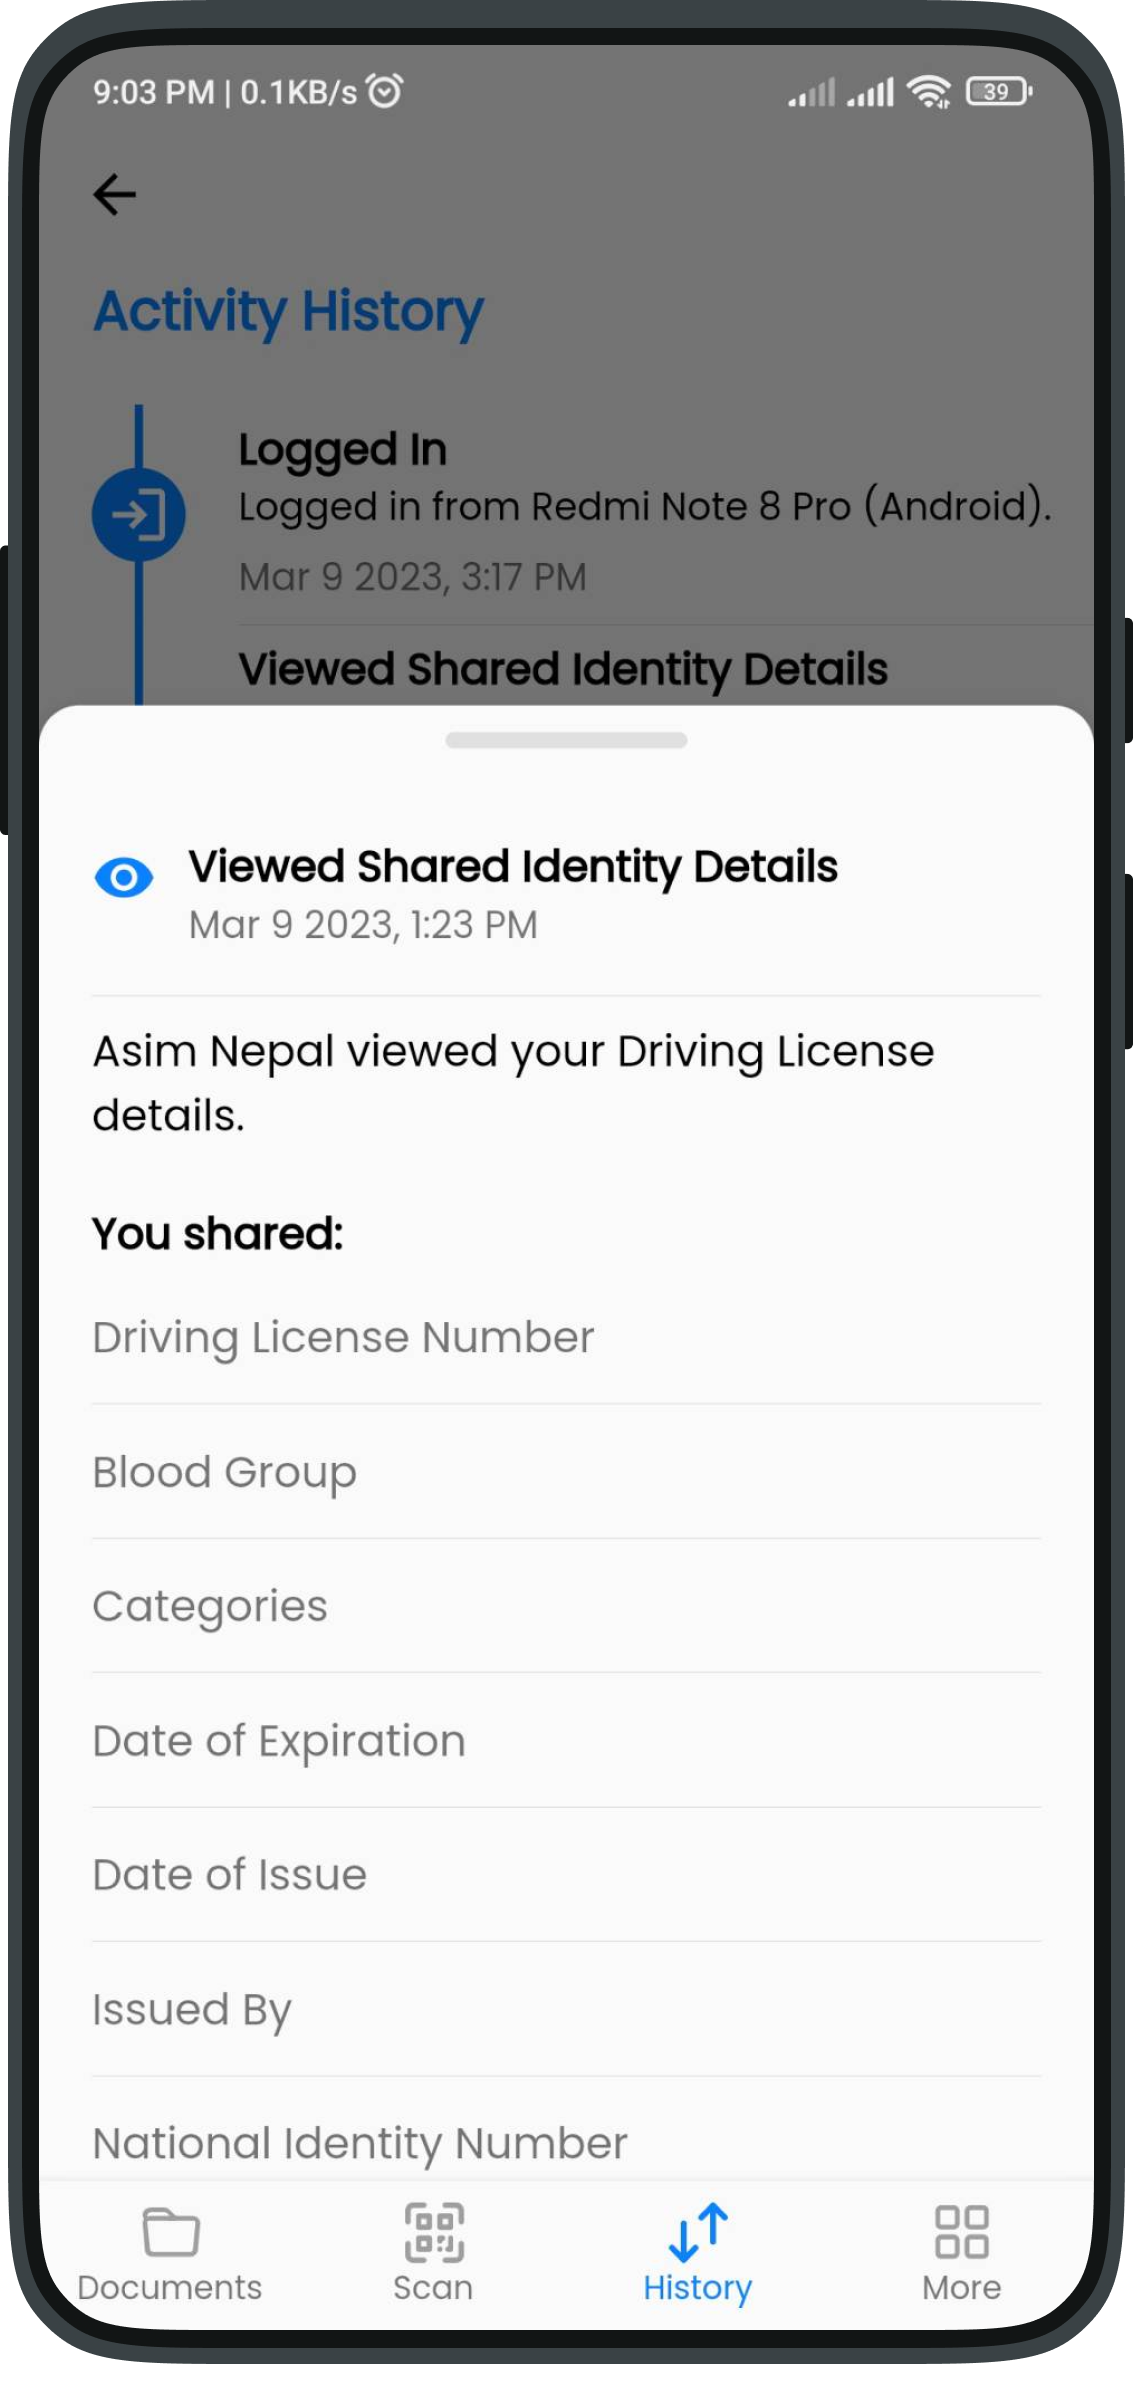
\includegraphics[width=0.6\linewidth]{images/results/mobile/HistoryDetails.png}
            \caption[History Log Details]{History Log Details}
            \label{fig:HistoryDetails.png}
            \end{figure}
        \end{multicols}
        
        \textbf{Other Features}\\
        Additional features and information of the app can be found in the more screen. Enabling or disabling dark mode, fingerprint to login, and logging out of the app are some of the features. 
        \begin{multicols}{2}
            \begin{figure}[H]
            \centering
            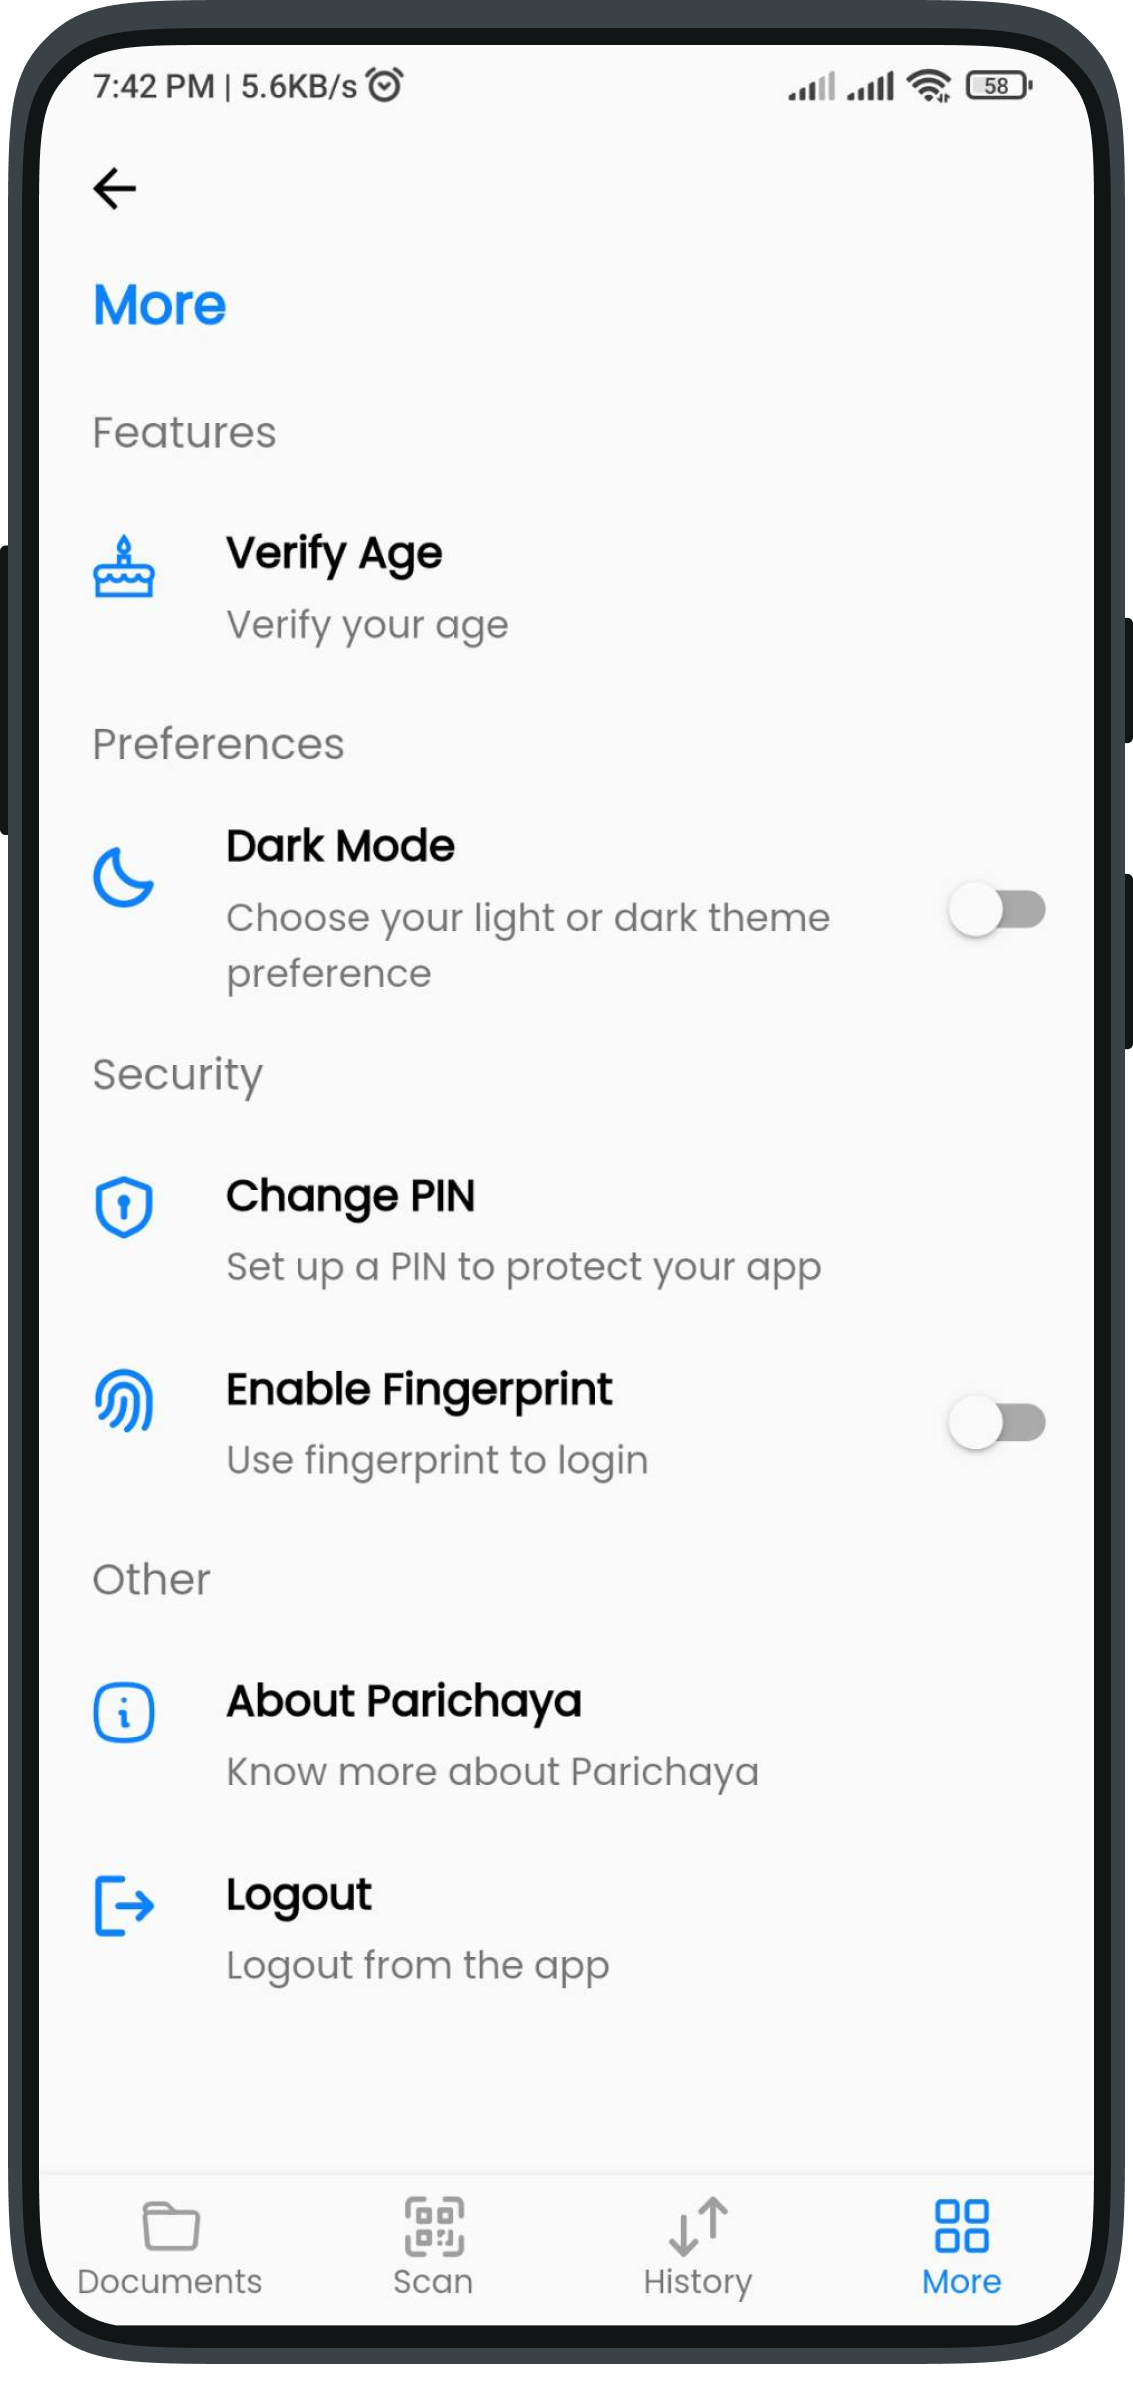
\includegraphics[width=0.6\linewidth]{images/results/mobile/More.png}
            \caption[More screen]{More Screen}
            \label{fig:More.png}
            \end{figure}     
            \begin{figure}[H]
            \centering
            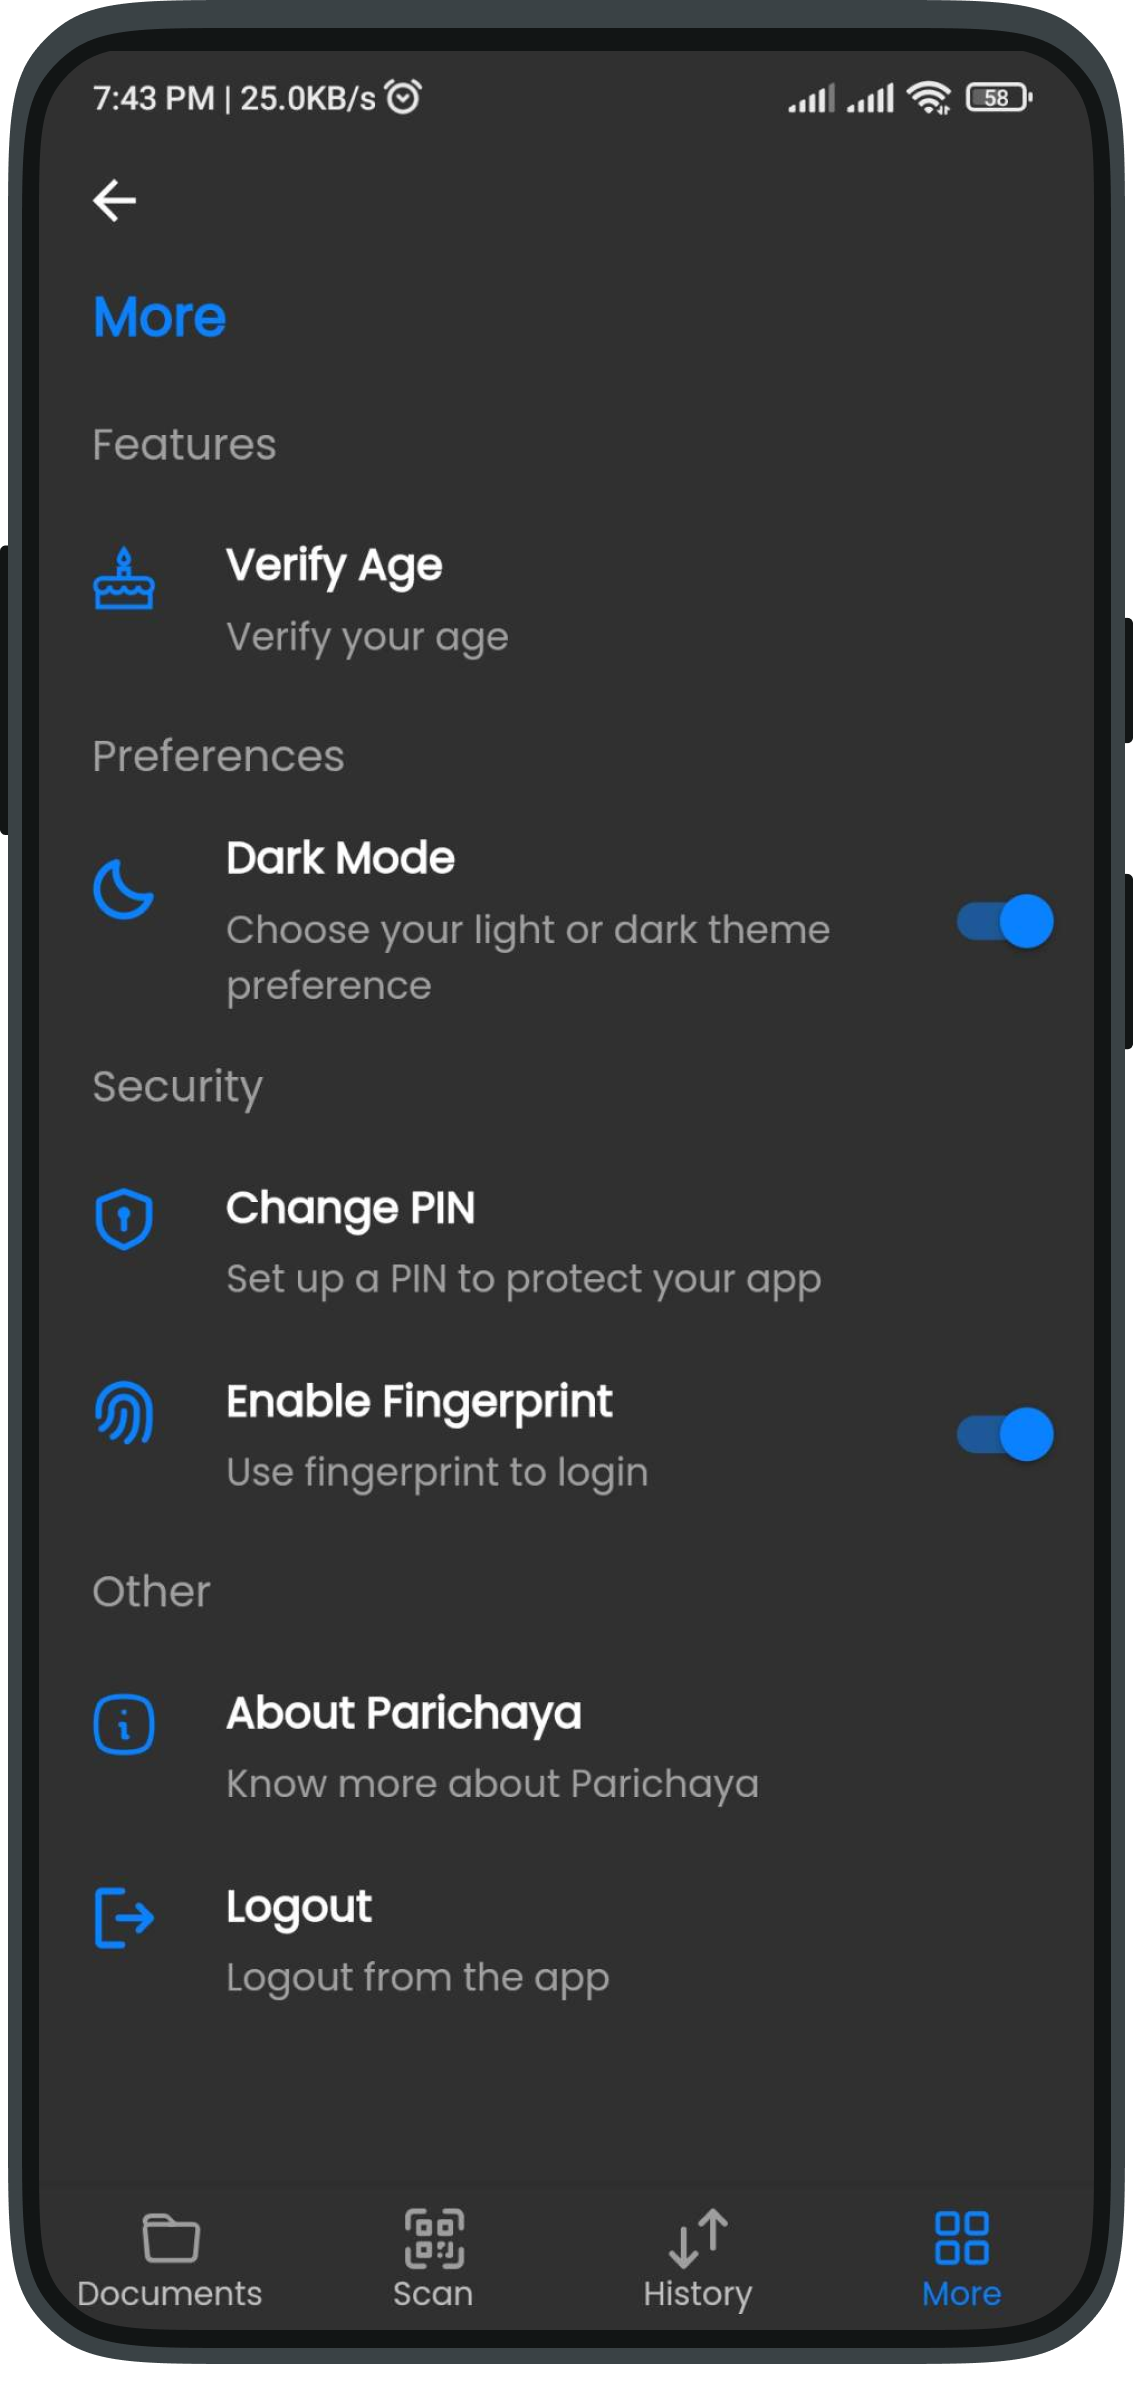
\includegraphics[width=0.6\linewidth]{images/results/mobile/MoreDarkMode.png}
            \caption[More Screen in Dark mode]{More Screen in Dark mode} 
            \label{fig:MoreDarkMode.png}
            \end{figure}
           \end{multicols}

           \textbf{Change MPIN}\\
           User can change their mpin when they are logged in either by scanning their fingerprint or by entering their previous mpin.
           
        \begin{multicols}{2}
            \begin{figure}[H]
            \centering
            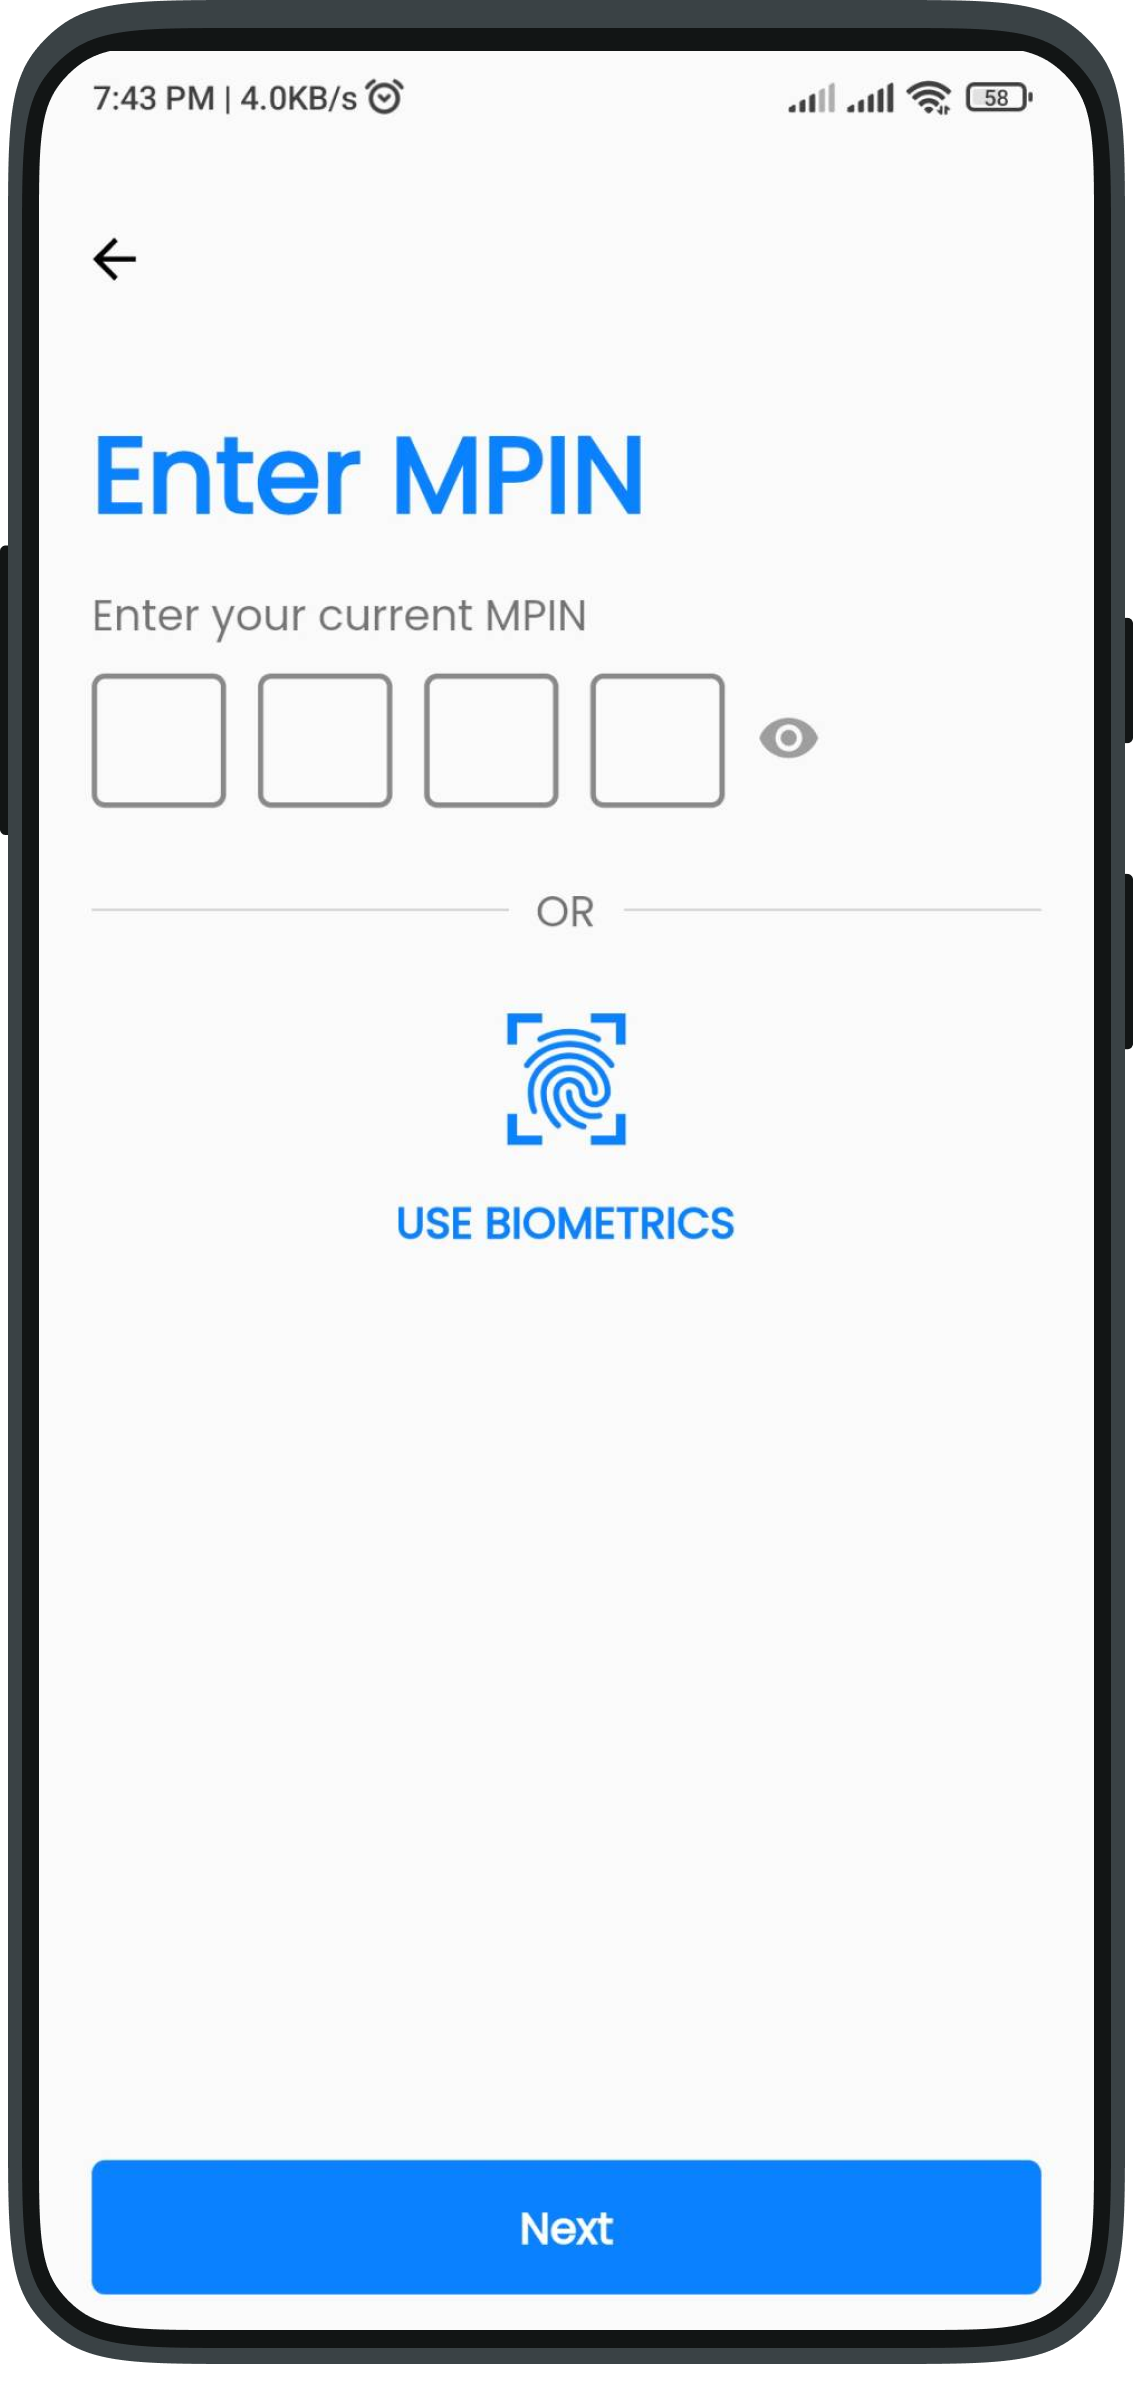
\includegraphics[width=0.6\linewidth]{images/results/mobile/ChangeMPIN.png}
            \caption[Enter Old MPIN Screen]{Enter Old MPIN Screen}
            \label{fig:ChangeMPIN.png}
            \end{figure}
            \begin{figure}[H]
            \centering
            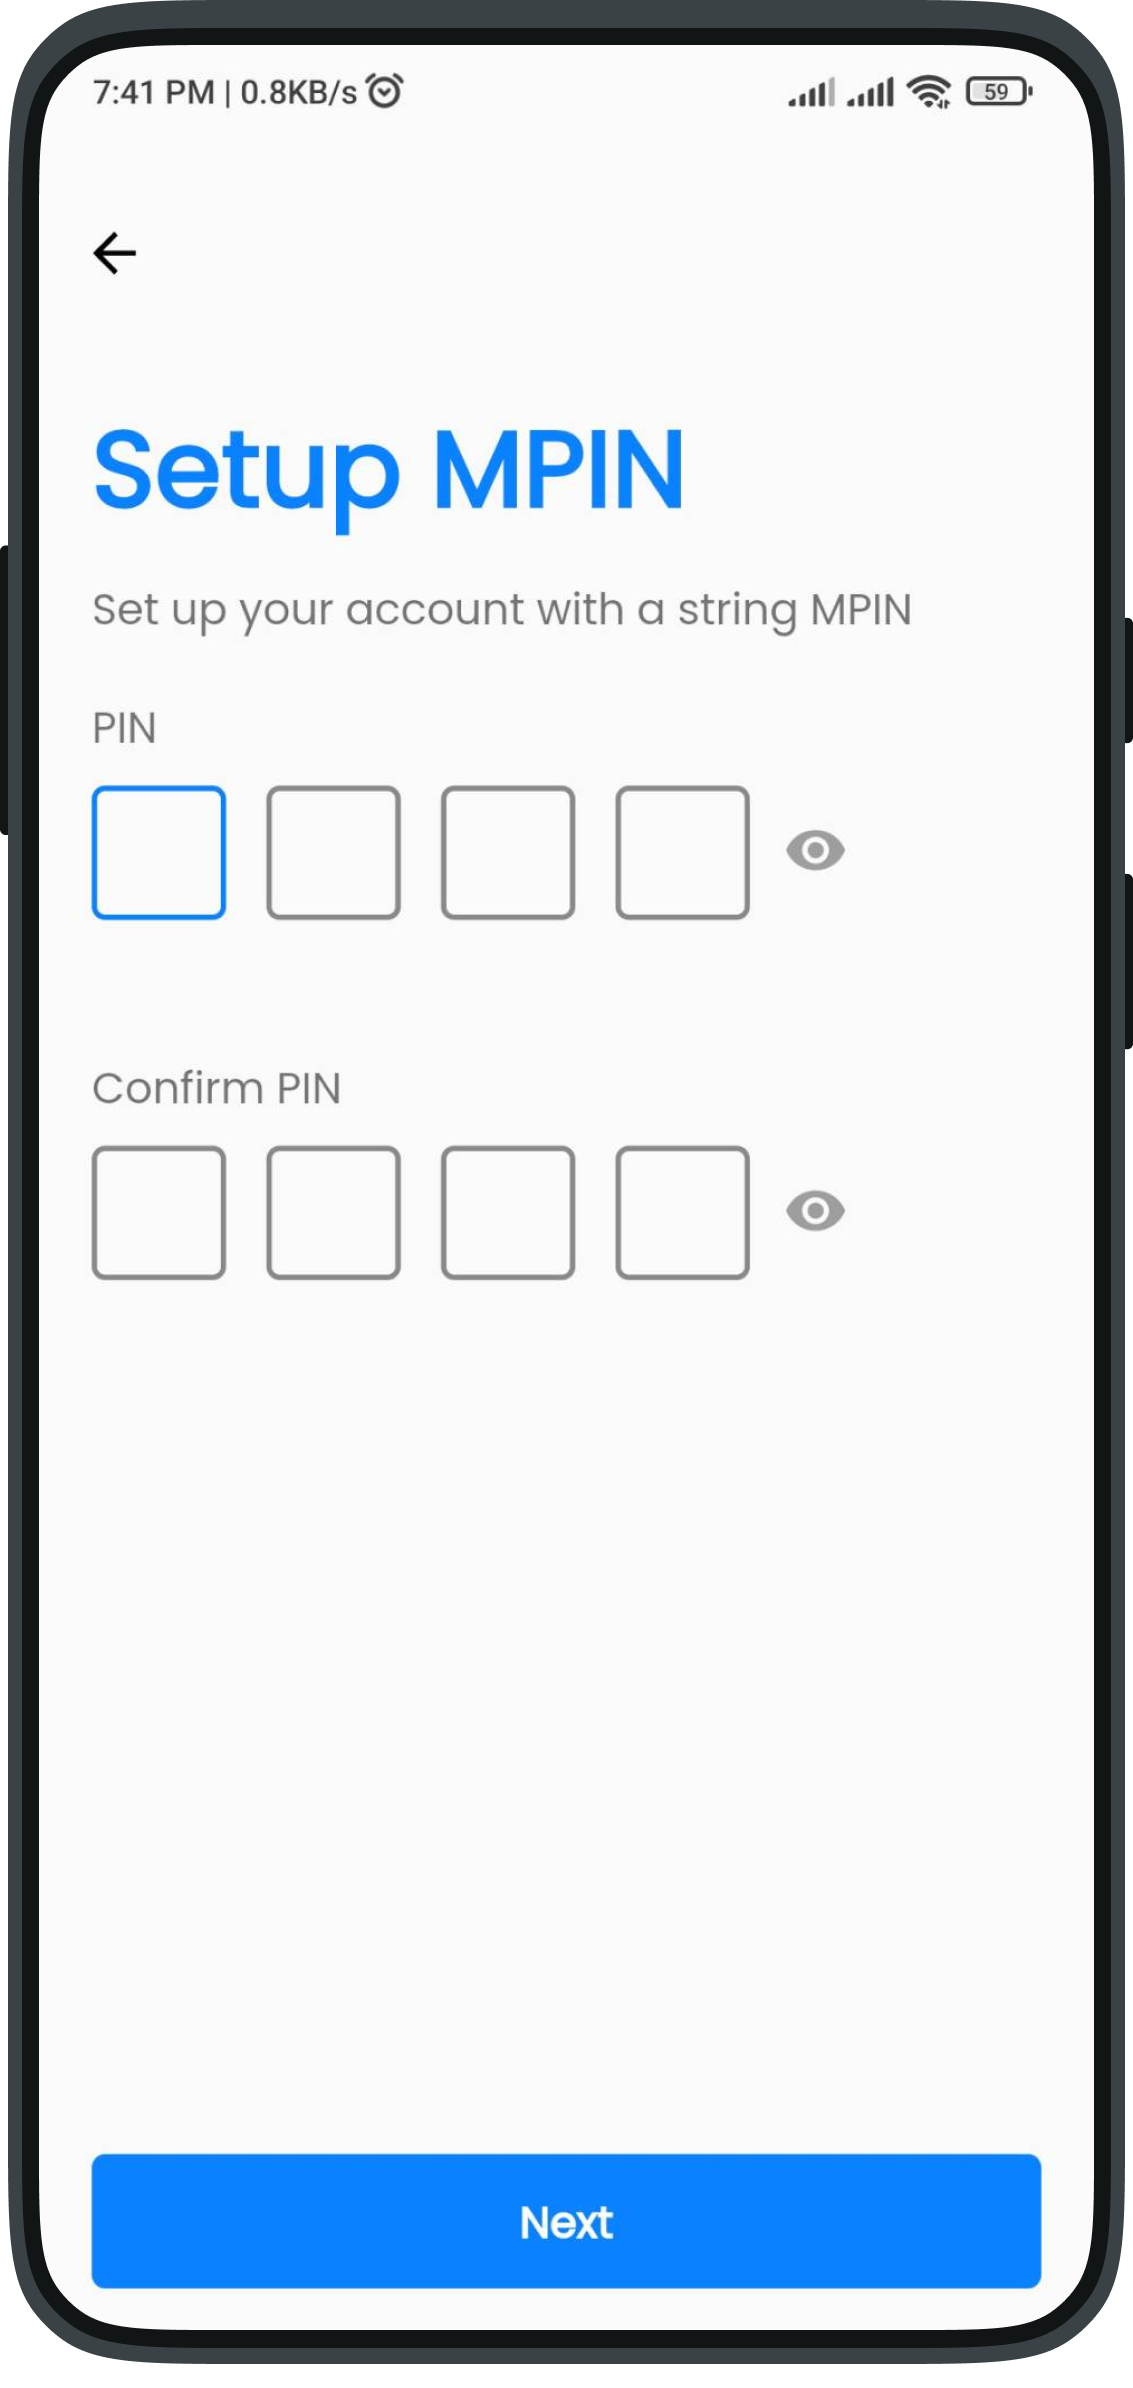
\includegraphics[width=0.6\linewidth]{images/results/mobile/SetupMPIN.png}
            \caption[Enter New MPIN Screen]{Enter New MPIN Screen}
            \label{fig:SetupMPIN.png}
            \end{figure}
        \end{multicols}

        \textbf{About Us}\\
         Users can learn more about the app and the developers who made it in the about us page. Users may view all the open source licenses that were used in the development of the app. Users may also gain knowledge about the developers by reading the team overview.
         \newpage
         \begin{multicols}{3}
            \begin{figure}[H]
            \centering
            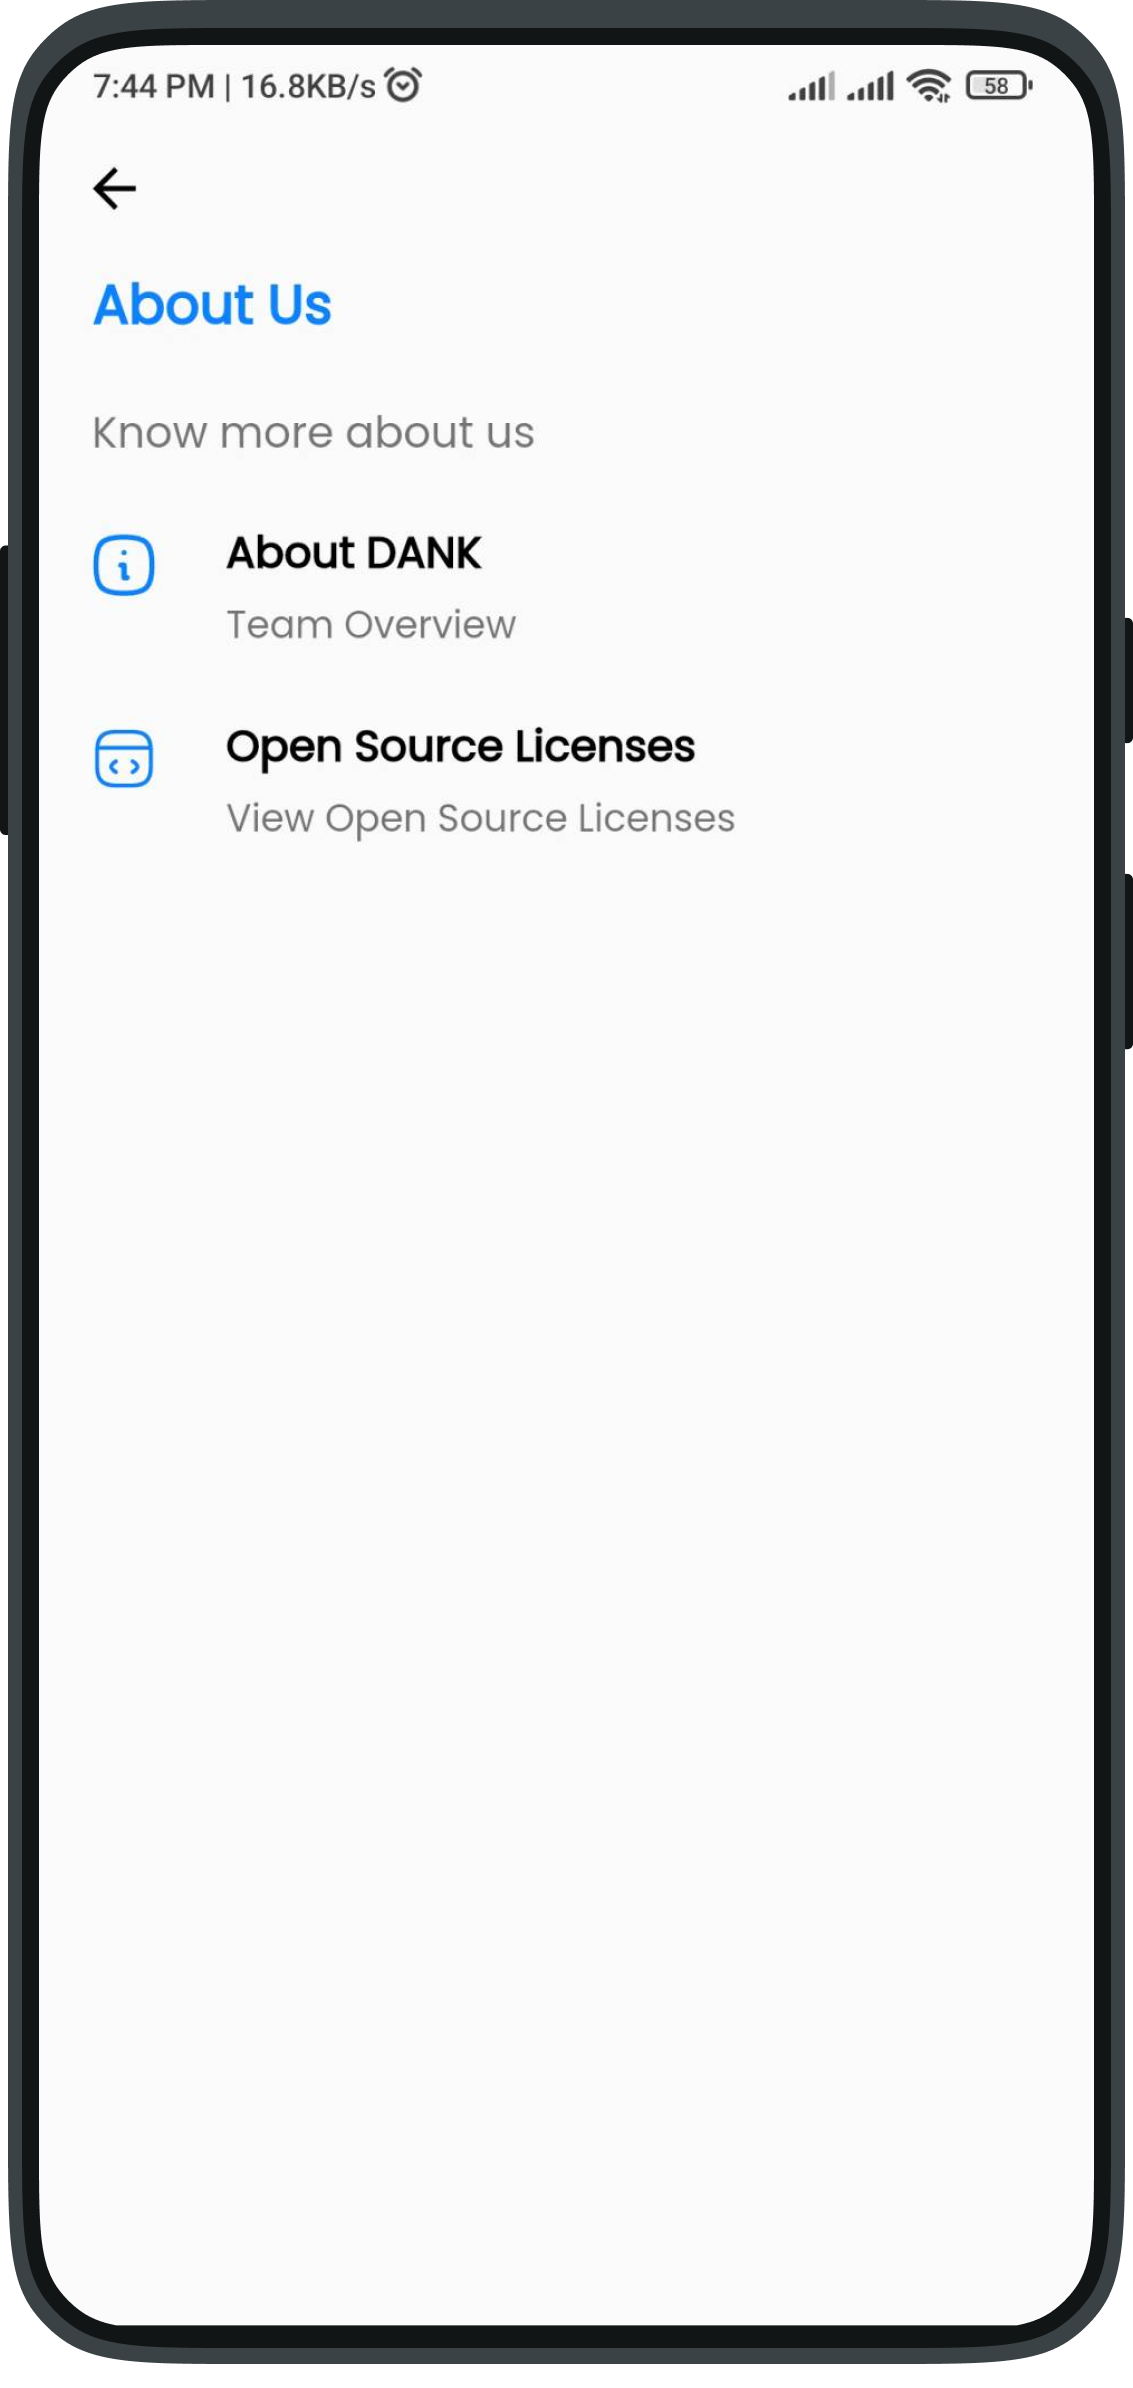
\includegraphics[width=0.85\linewidth]{images/results/mobile/AboutUs.png}
            \caption[About Us]{About Us}
            \label{fig:AboutUs.png}
            \end{figure}     
            \begin{figure}[H]
            \centering
            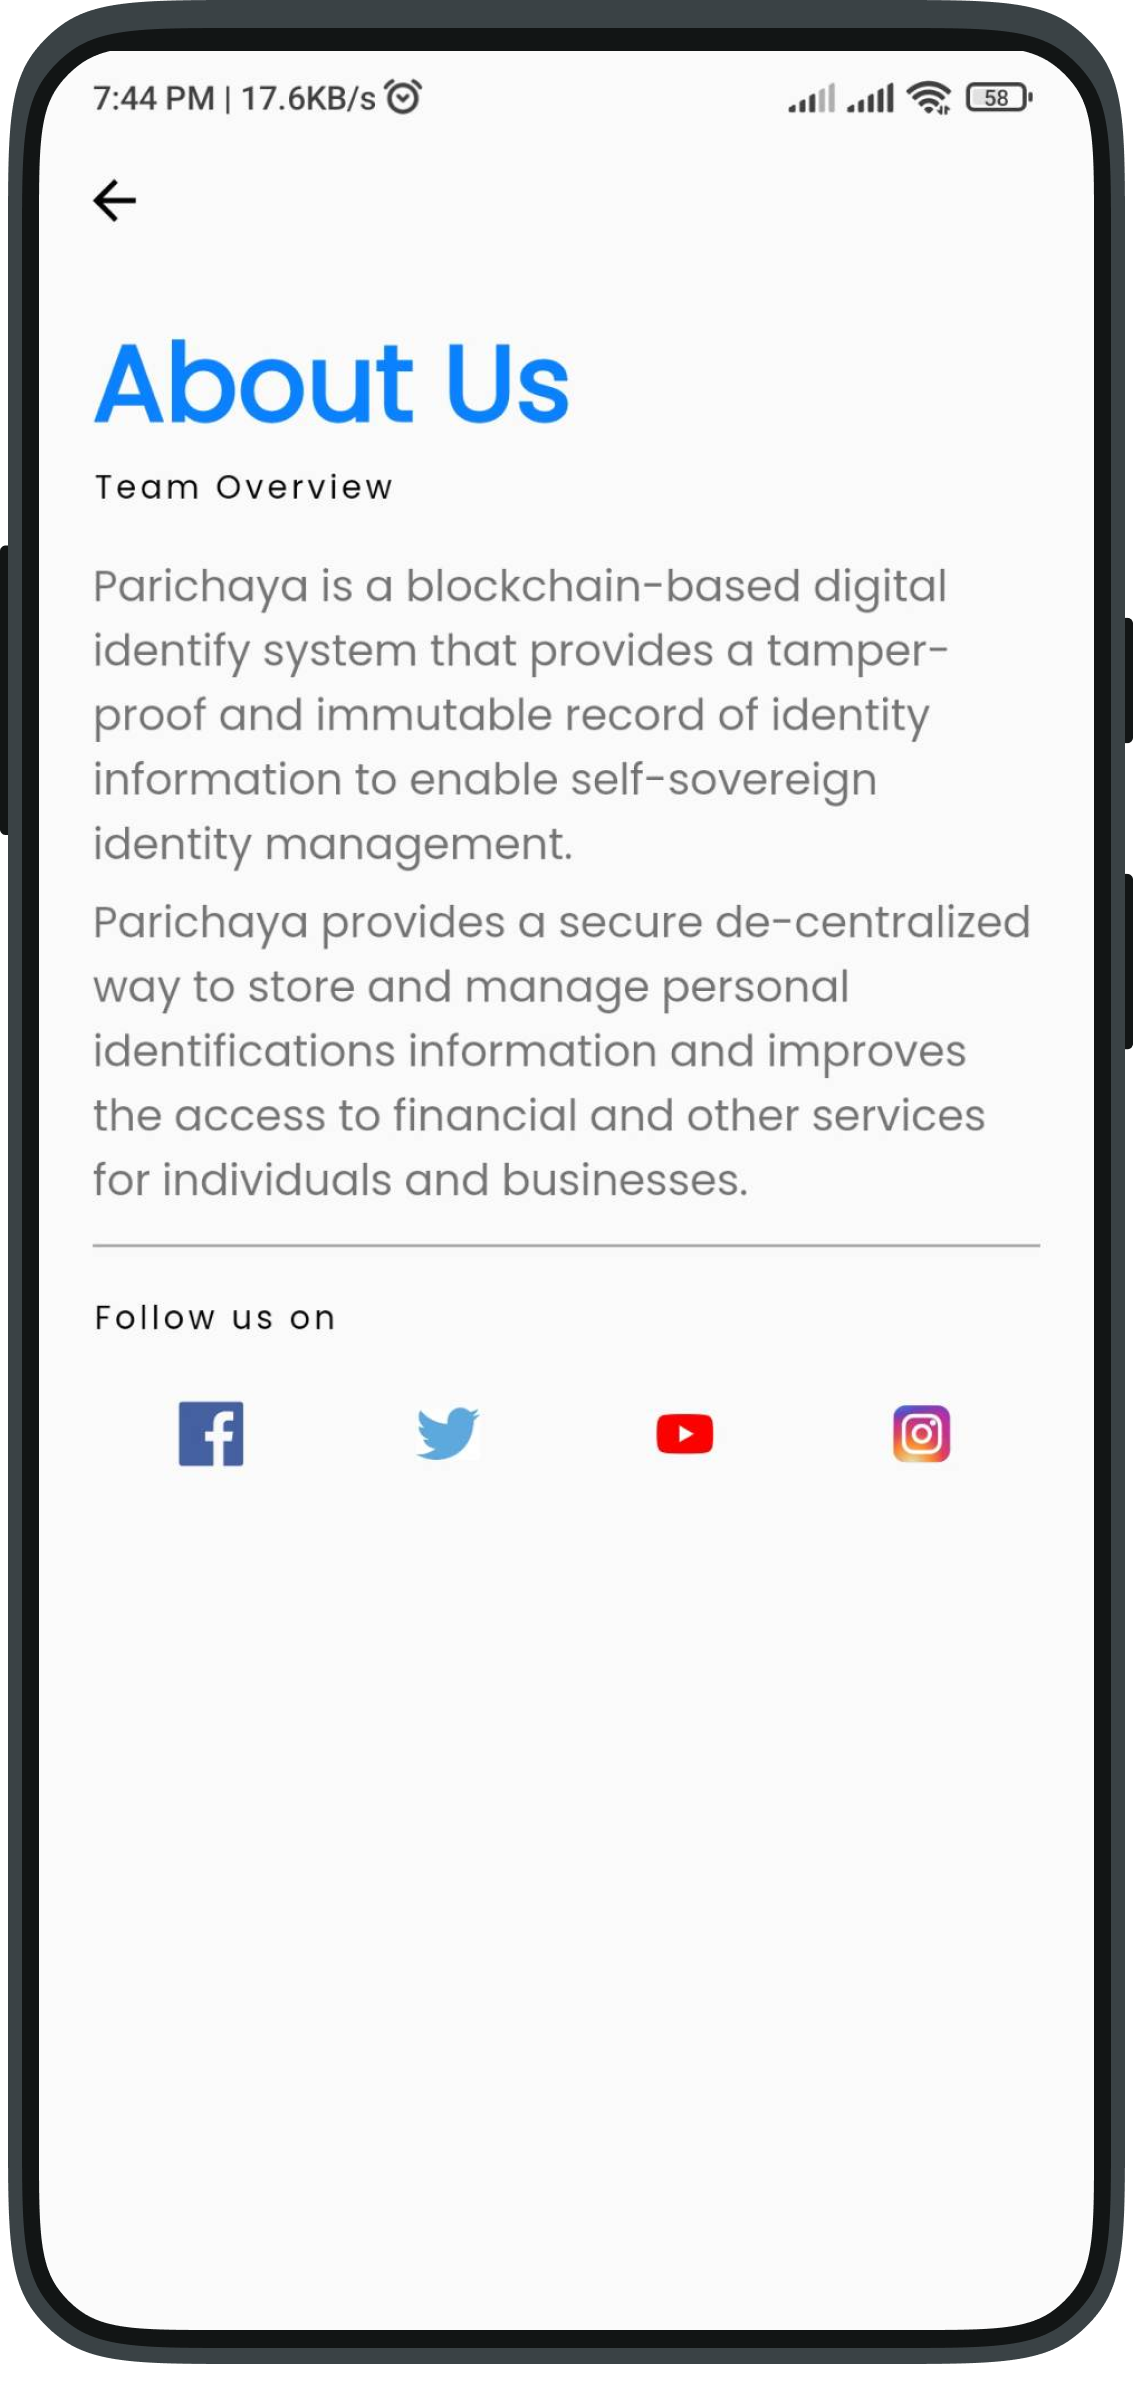
\includegraphics[width=0.85\linewidth]{images/results/mobile/TeamOverview.png}
            \caption[About Dank]{About Dank}
            \label{fig:TeamOverview.png}
            \end{figure}
            \begin{figure}[H]
            \centering
            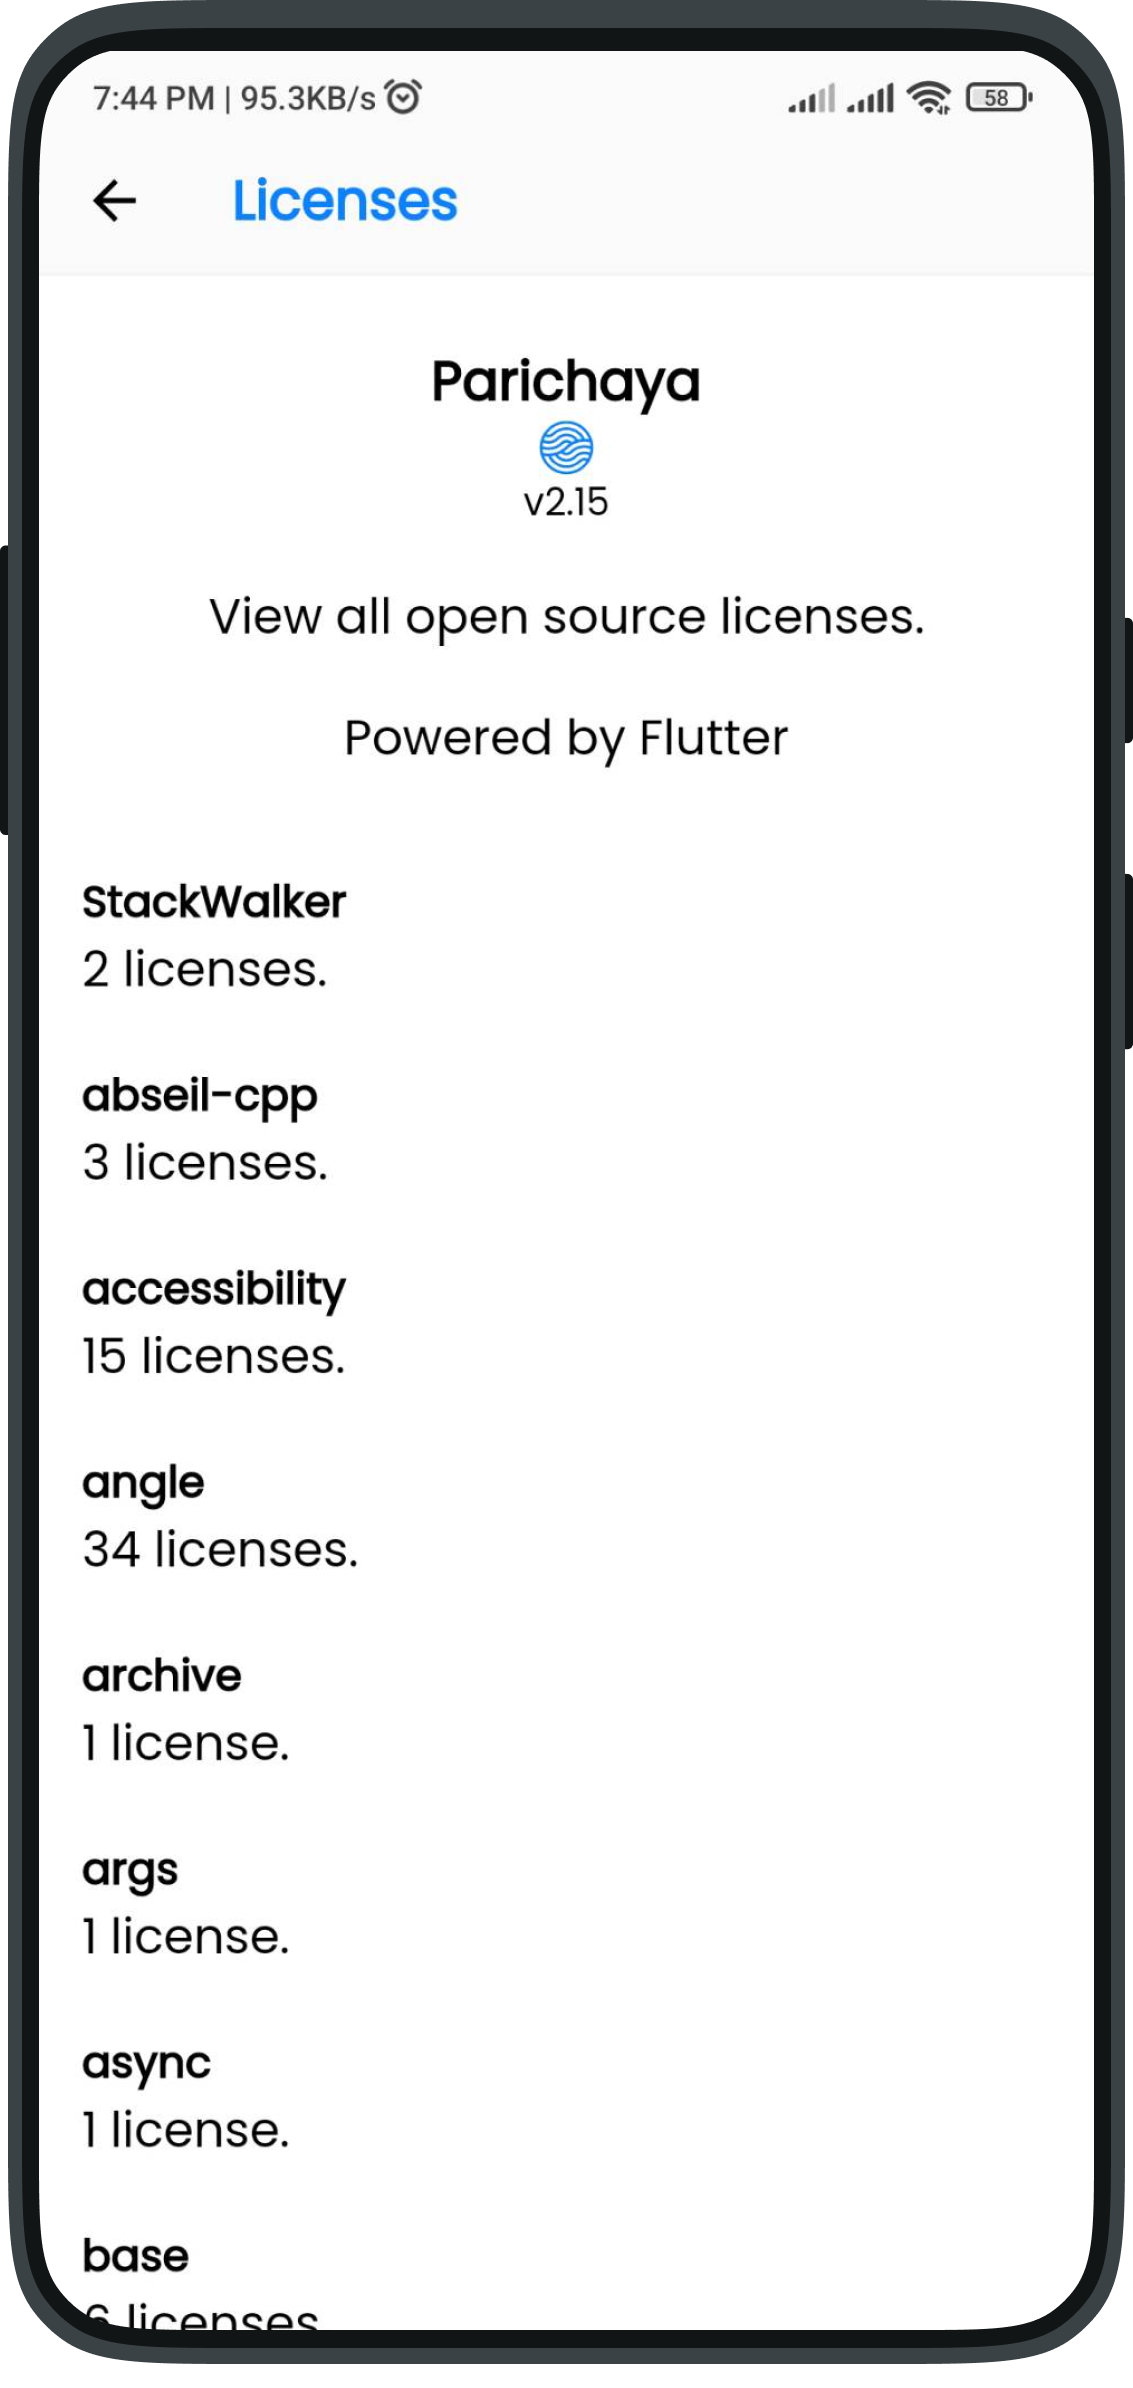
\includegraphics[width=0.85\linewidth]{images/results/mobile/OpenSourceLicenses.png}
            \caption[License]{License}
            \label{fig:OpenSourceLicenses.png}
            \end{figure}
        
        \end{multicols}

        \textbf{Log Out}\\
        When user log outs of the application.
         \begin{figure}[H]
            \centering
            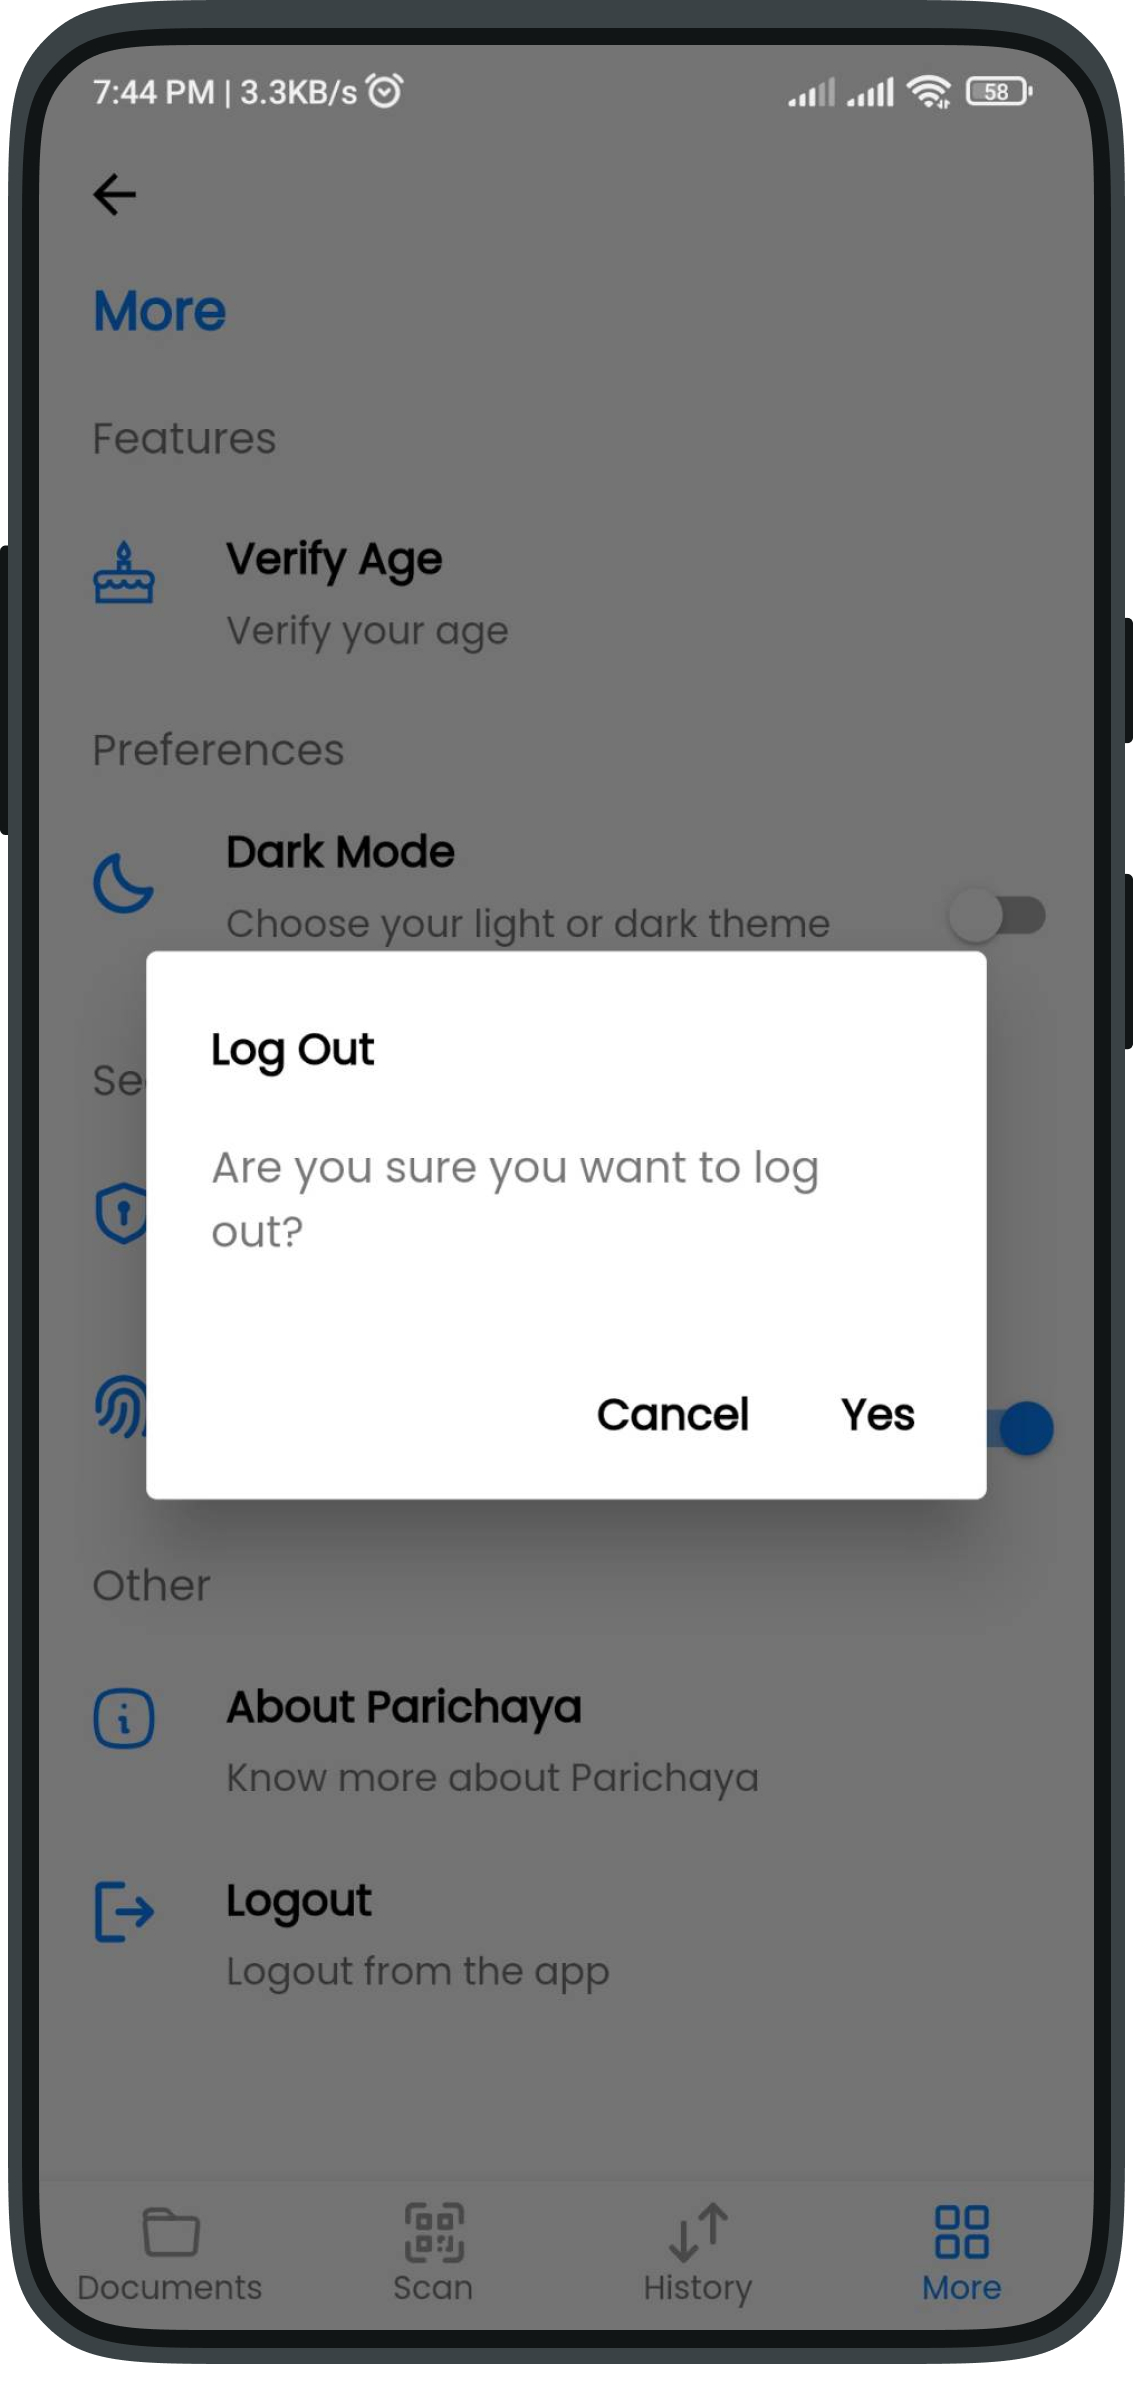
\includegraphics[width=0.3\linewidth]{images/results/mobile/Logout.png}
            \caption[Logout]{Logout}
            \label{fig:Logout.png}
            \end{figure}

       
     
\subsection{Website Application}
  Employee of government working on issuing national identity, citizenship and driving license who is register in database can log in to the portal by giving correct username and their password.

        \begin{figure}[H]
        \centering
        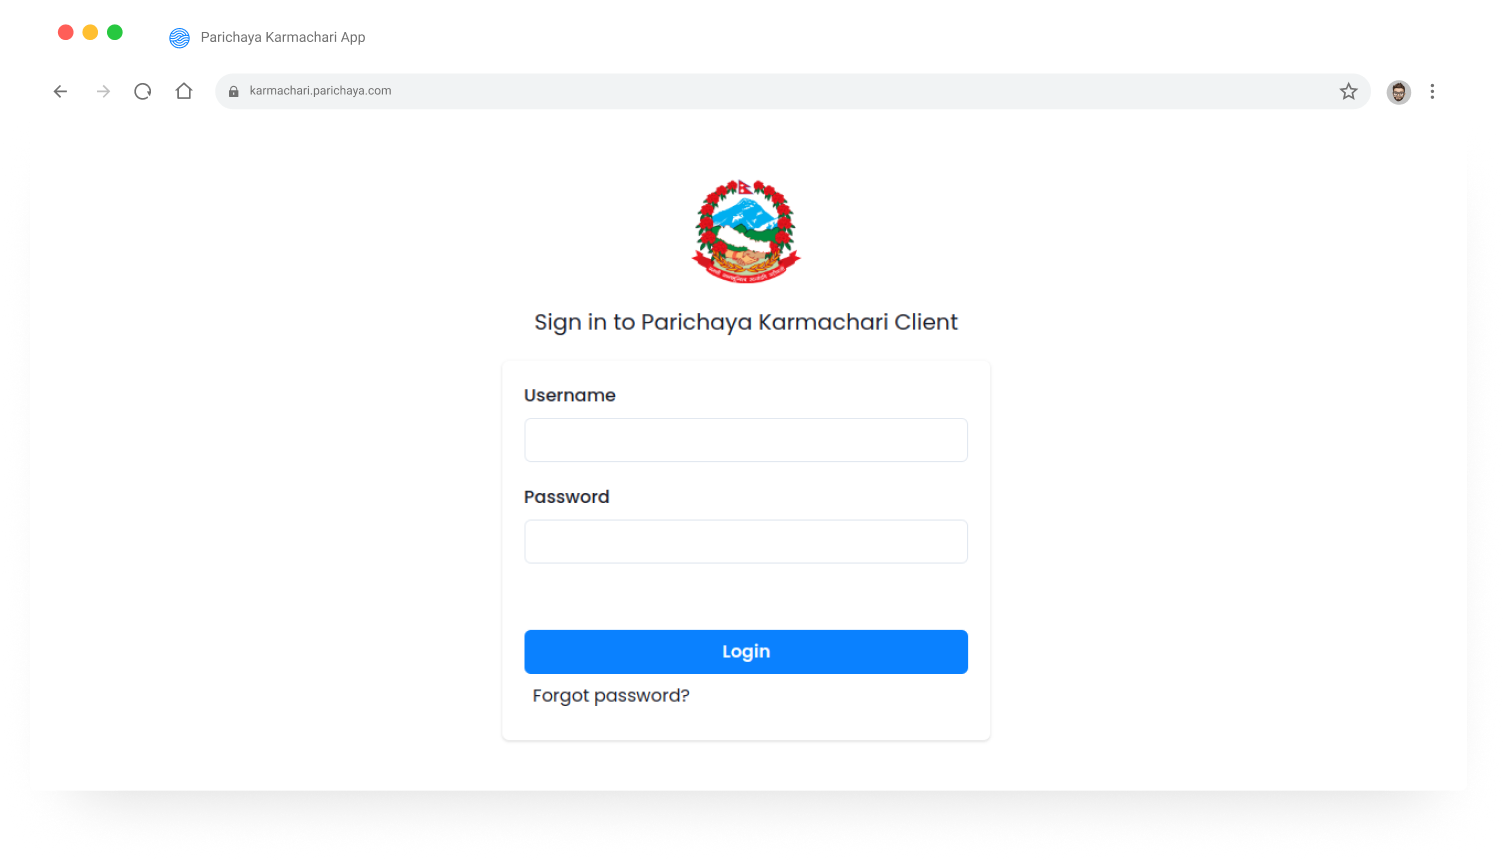
\includegraphics[width=0.6\linewidth]{images/results/web/WebLoginPage.png}
        \caption[Login]{Login}
        \label{fig:WebLoginPage.png}
        \end{figure}

           \begin{figure}[H]
        \centering
        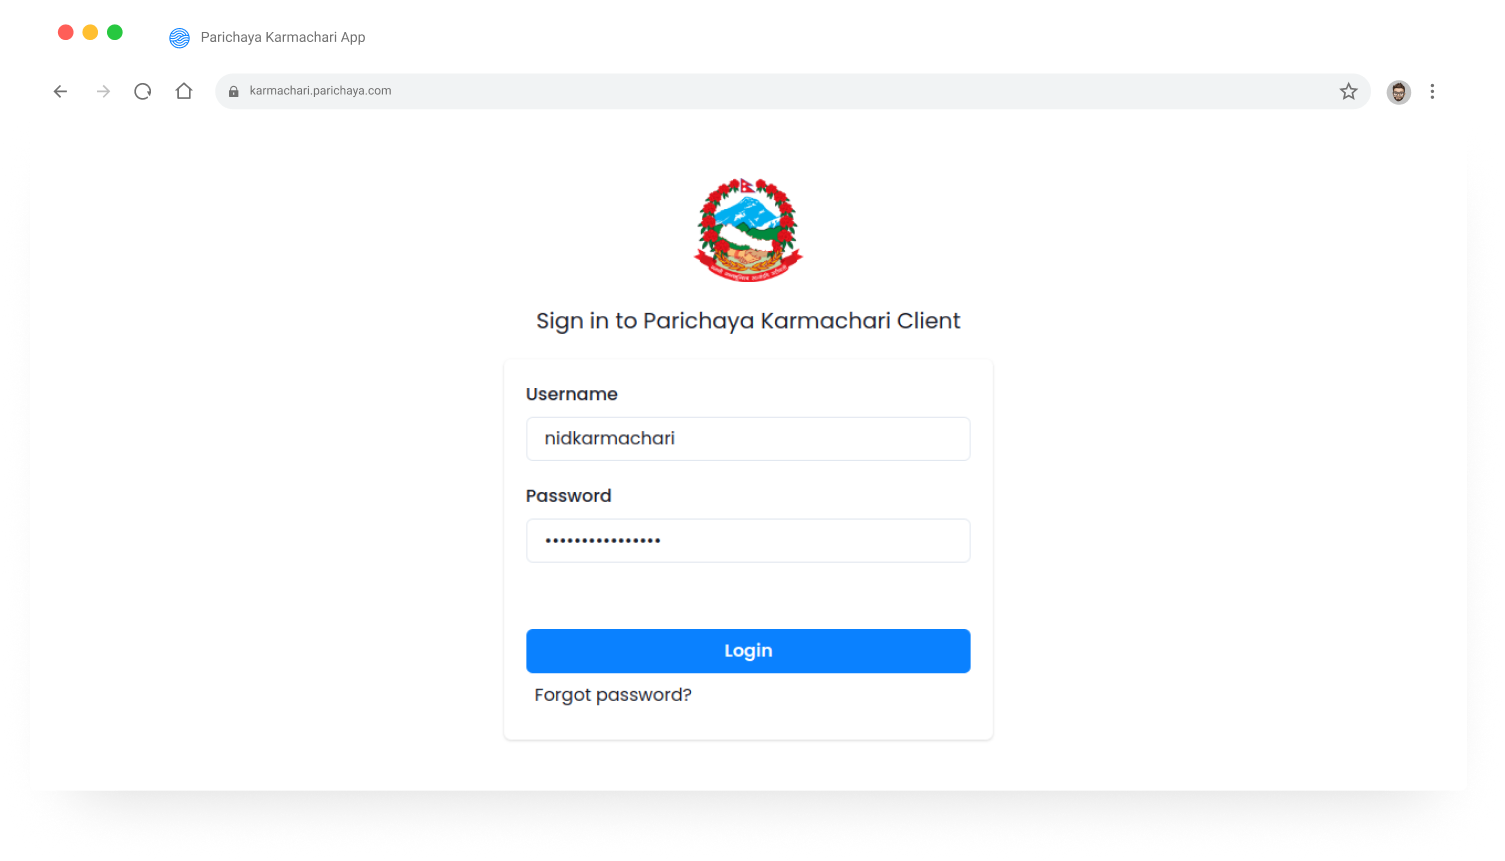
\includegraphics[width=0.6\linewidth]{images/results/web/FilledWebLogin.png}
        \caption[Filled Login]{Filled Login}
        \label{fig:FilledWebLogin.png}
        \end{figure}

   
    

     \begin{figure}[H]
        \centering
        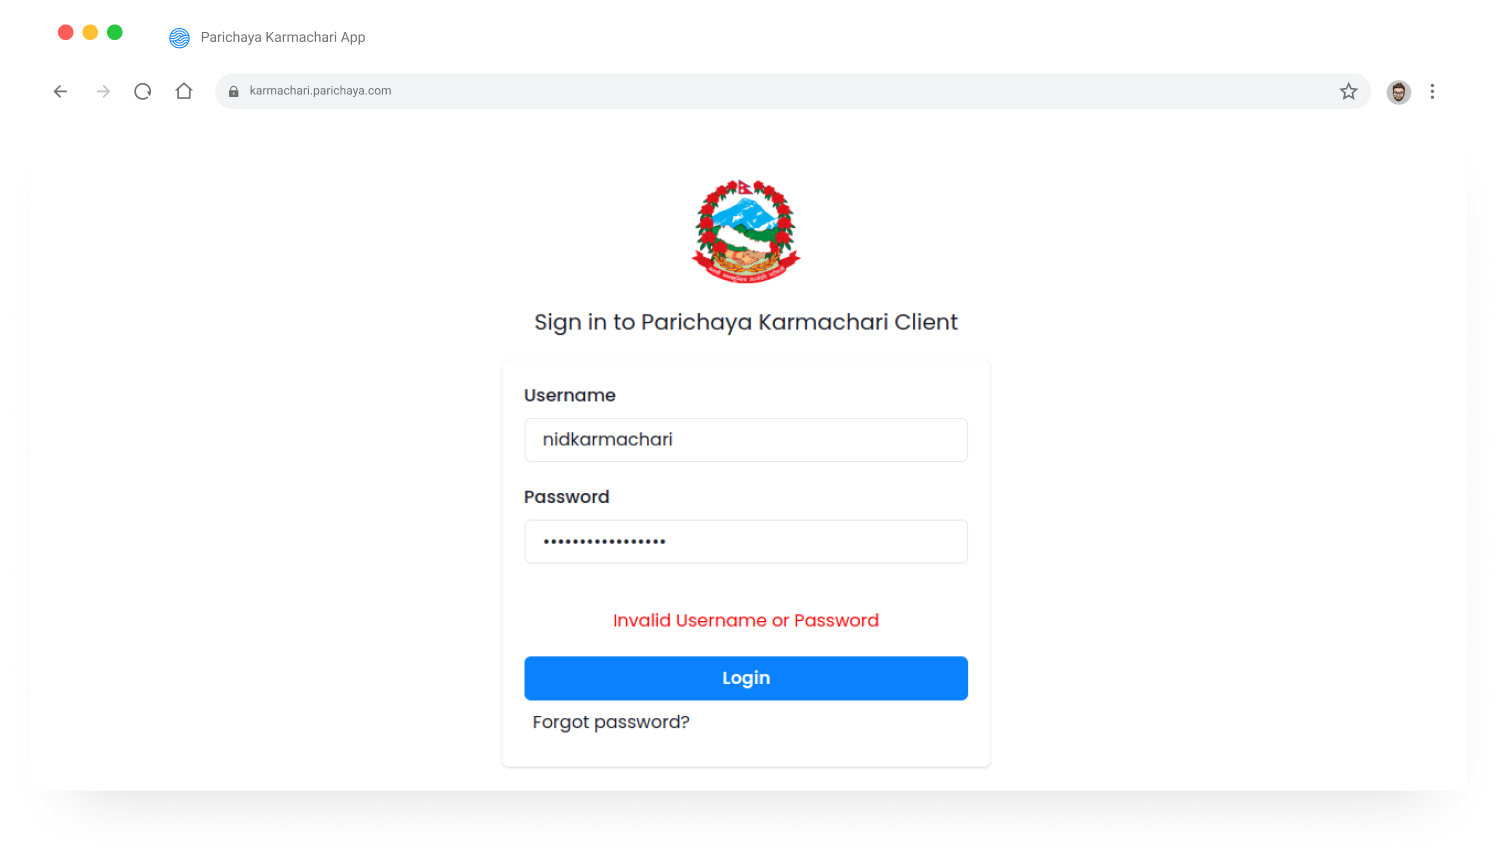
\includegraphics[width=0.6\linewidth]{images/results/web/WebLoginErrorPage.png}
        \caption[Login Error page ]{Login Error page}
        \label{fig:WebLoginErrorPage.png}
        \end{figure}
    Government Employee after logging in get to the home page. Here they can search for various identity documents like national identity card, citizenship card and driving license of any citizen based on their national identity number.In the left side of the homepage, there is vertical navigation bar which contains homepage, National identity card, Citizenship Card and Driving License.

        \begin{figure}[H]
        \centering
        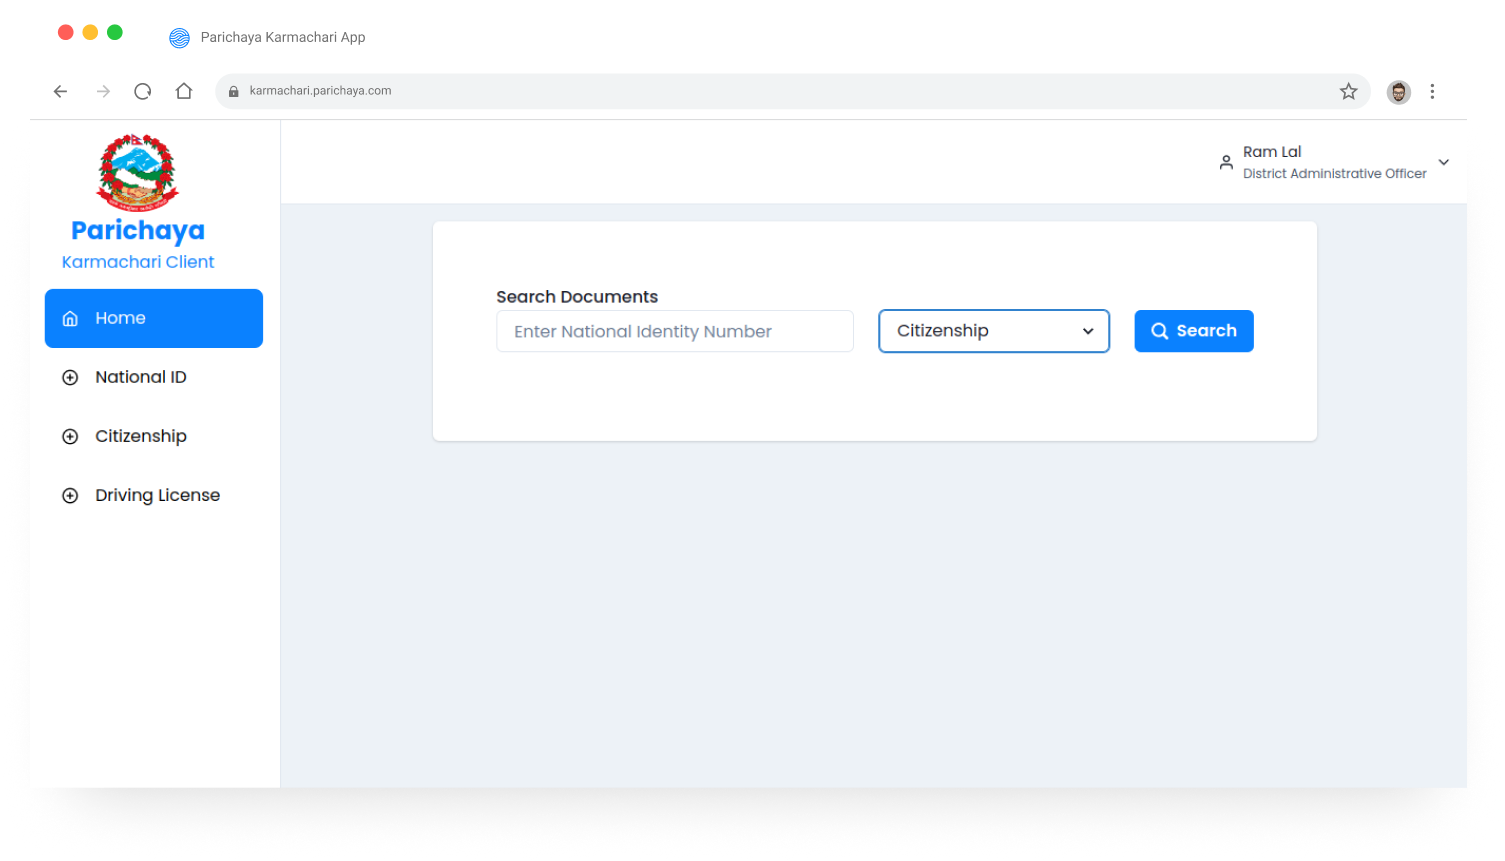
\includegraphics[width=0.8\linewidth]{images/results/web/WebHomePage.png}
      \caption[Home Page]{Home Page}
        \label{fig:WebHomePage.png}
        \end{figure}

           \begin{figure}[H]
        \centering
        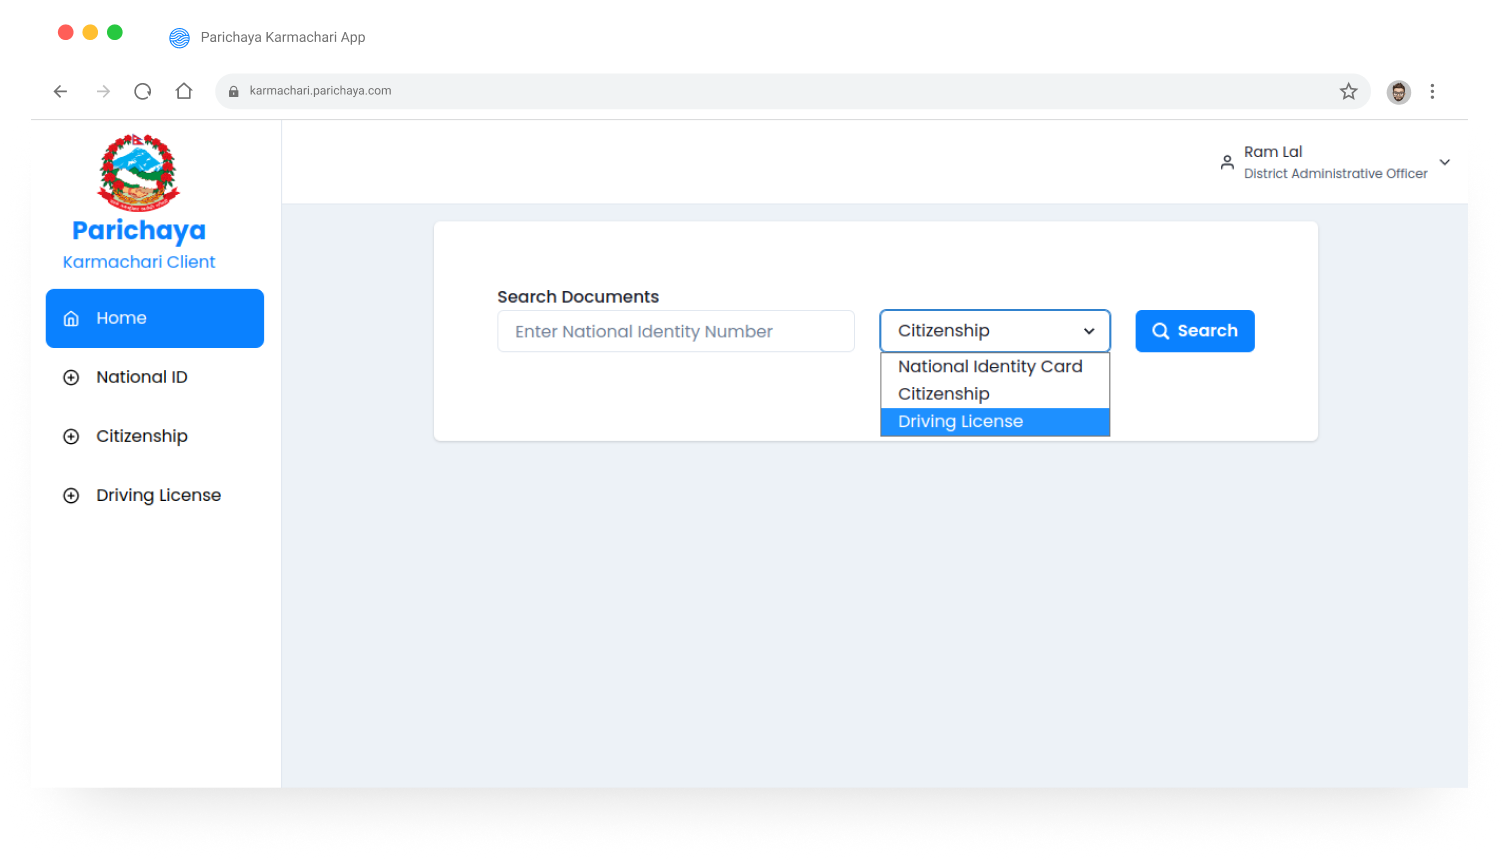
\includegraphics[width=0.8\linewidth]{images/results/web/WebHomePage2.png}
        \caption[Filled Home Page]{Filled Home Page}
        \label{fig:WebHomePage2.png}
        \end{figure}

           \begin{figure}[H]
        \centering
        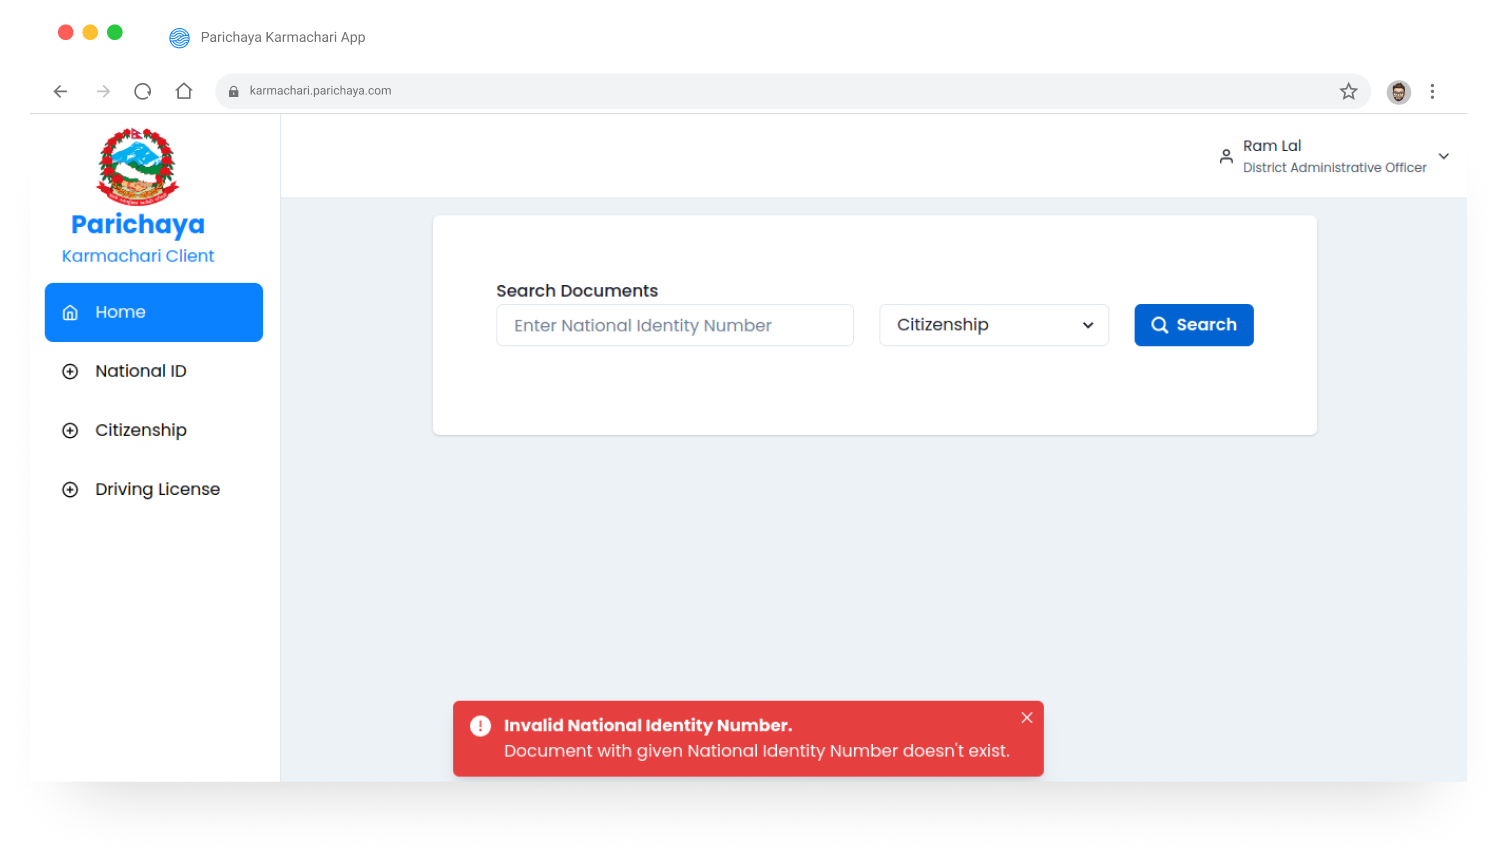
\includegraphics[width=0.8\linewidth]{images/results/web/WebHomeError.png}
        \caption[Home error Page ]{Home error Page }
        \label{fig:WebHomeError.png}
        \end{figure}


    By clicking on National ID in the vertical navbar, we go to National identity registration page where we can register NID card for citizens. 
   
        \begin{figure}[H]
        \centering
        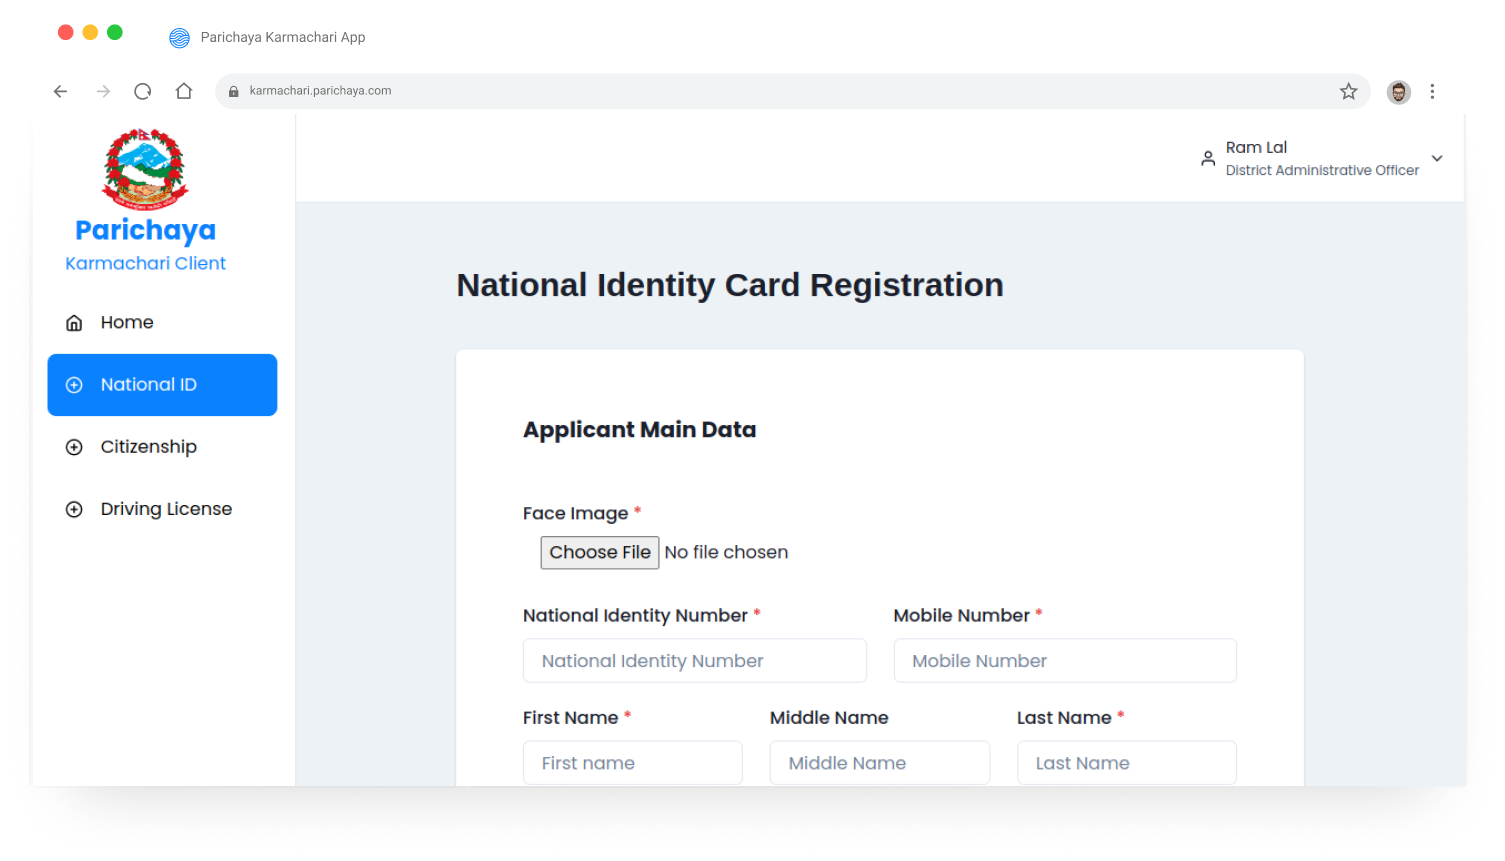
\includegraphics[width=0.8\linewidth]{images/results/web/WebNationalIDCardRegistration1.png}
        \caption[National ID Form]{National ID Form}
        \label{fig:WebNationalIDCardRegistration1.png}
        \end{figure}

           \begin{figure}[H]
        \centering
        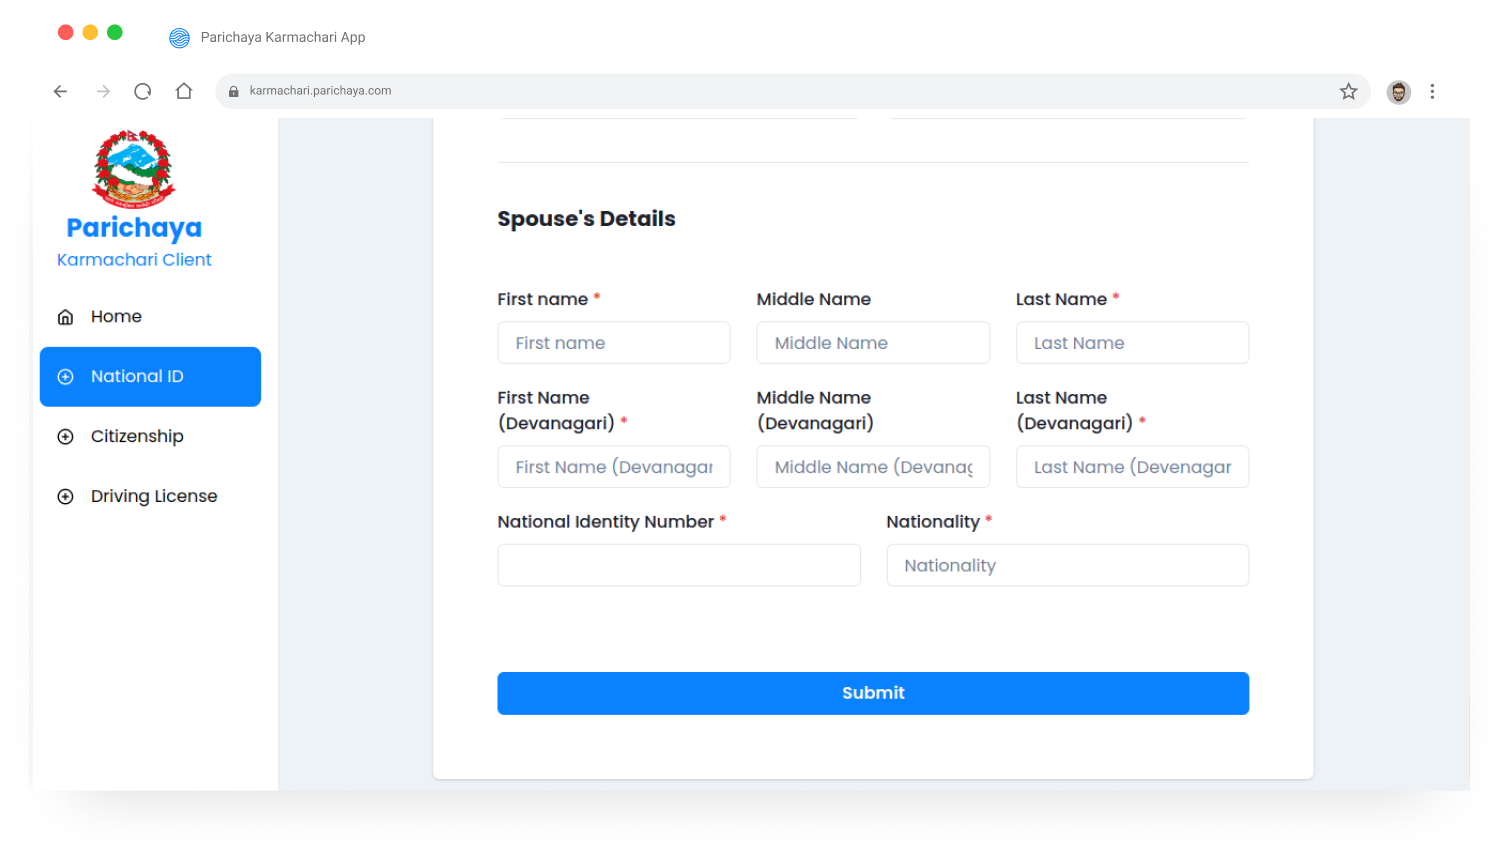
\includegraphics[width=0.8\linewidth]{images/results/web/WebNationalIDCardRegistration2.png}
        \caption[National ID Form]{National ID Form}
        \label{fig:WebNationalIDCardRegistration2.png}
        \end{figure}

    In this project, every identity documents is tied to National Identity Number. Therefore, before accessing any identity documents of a user, his National identity number has to be filled first. Then Government Employee can access other identity documents. They can make changes to the identity documents if needed as well. 


        \begin{figure}[H]
        \centering
        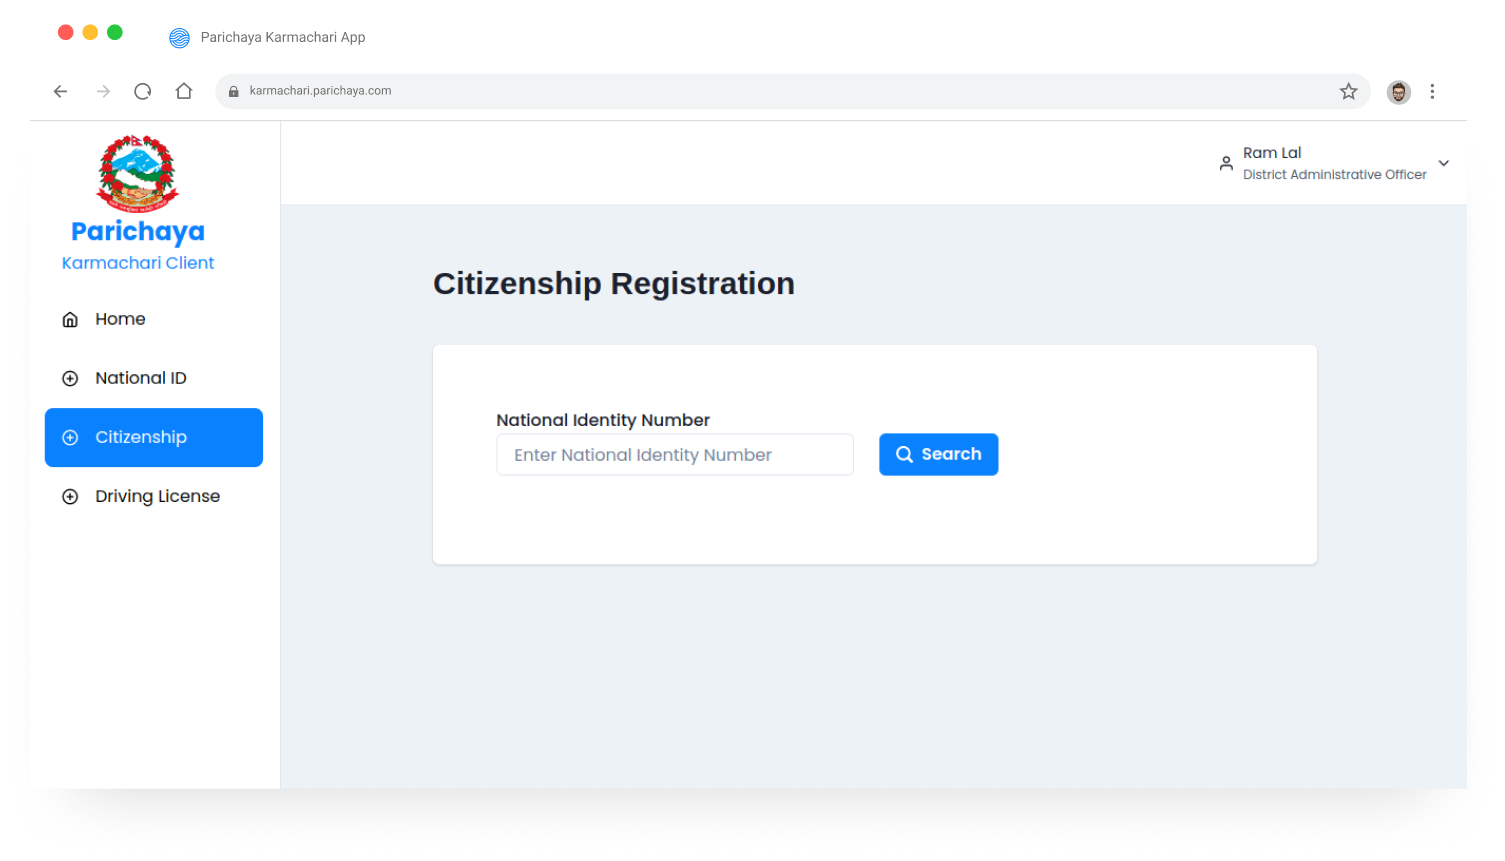
\includegraphics[width=0.8\linewidth]{images/results/web/WebCitizenshipRegistration1.png}
        \caption[Enter NIN]{Enter NIN}
        \label{fig:WebCitizenshipRegistration1.png}
        \end{figure}

           \begin{figure}[H]
        \centering
        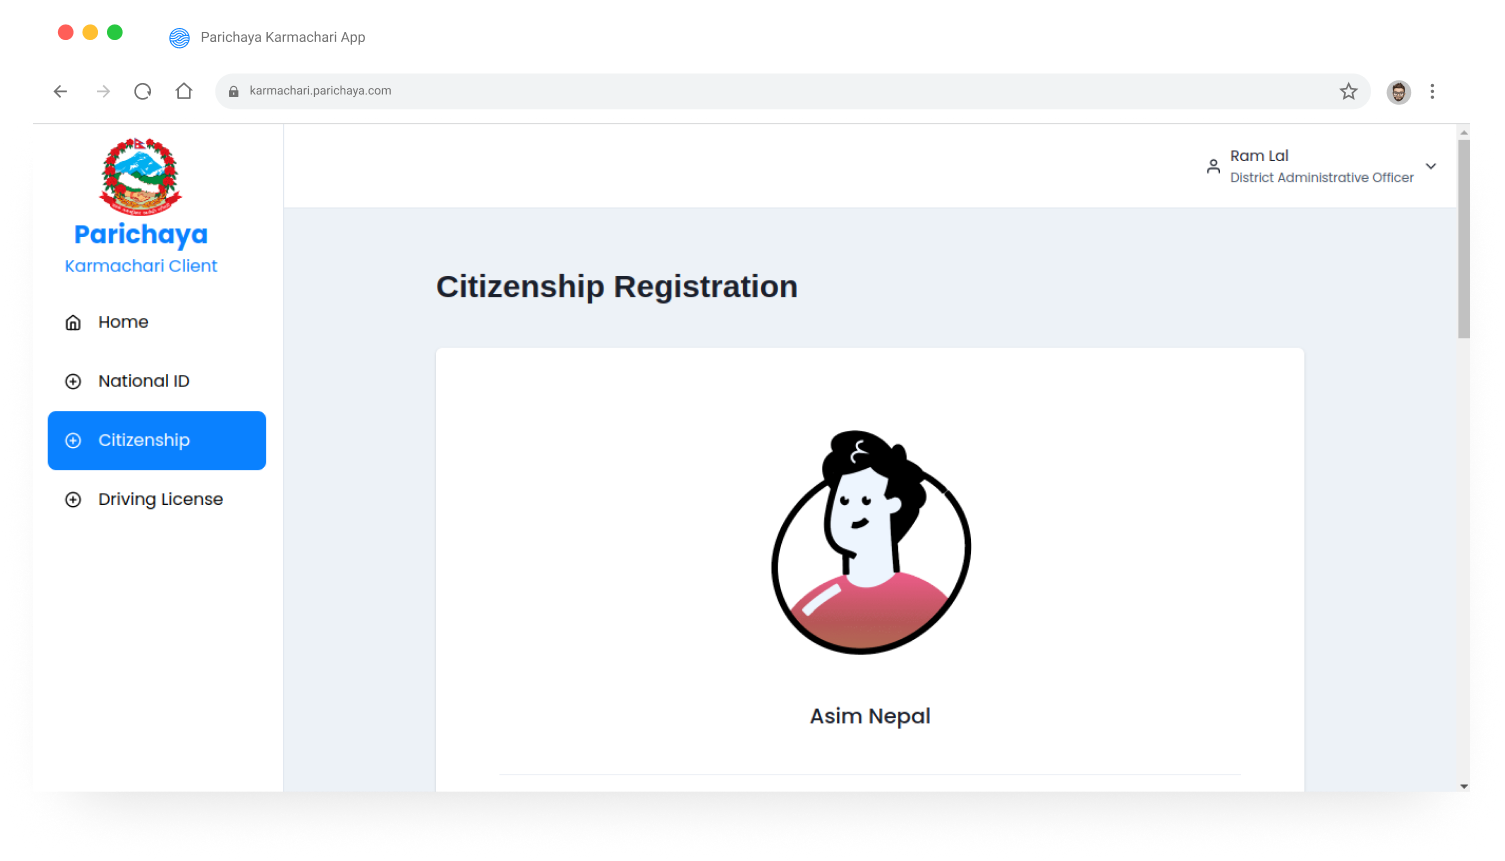
\includegraphics[width=0.8\linewidth]{images/results/web/WebCitizenshipRegistration2.png}
        \caption[Citizenship Card Form]{Citizenship Card Form}
        \label{fig:WebCitizenshipRegistration2.png}
        \end{figure}

          \begin{figure}[H]
        \centering
        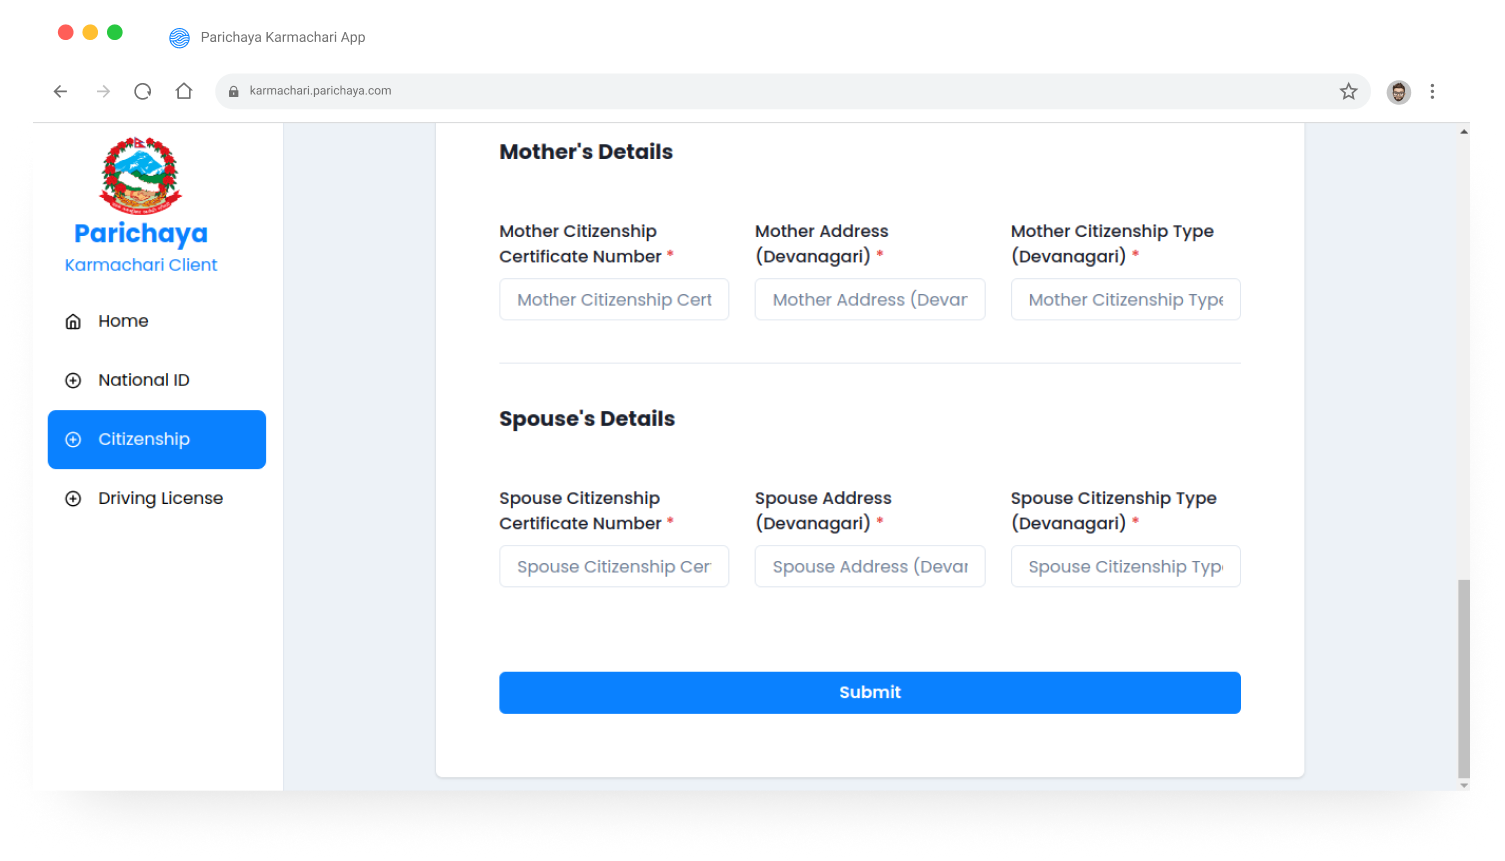
\includegraphics[width=0.8\linewidth]{images/results/web/WebCitizenshipRegistration3.png}
        \caption[Citizenship Card Form]{Citizenship Card Form}
        \label{fig:WebCitizenshipRegistration3.png}
        \end{figure}
    Similar to Citizenship card, to fill form or to access driving license or to make changes in the driving license,initially, National identity number of the citizen should be filled. 

        \begin{figure}[H]
        \centering
        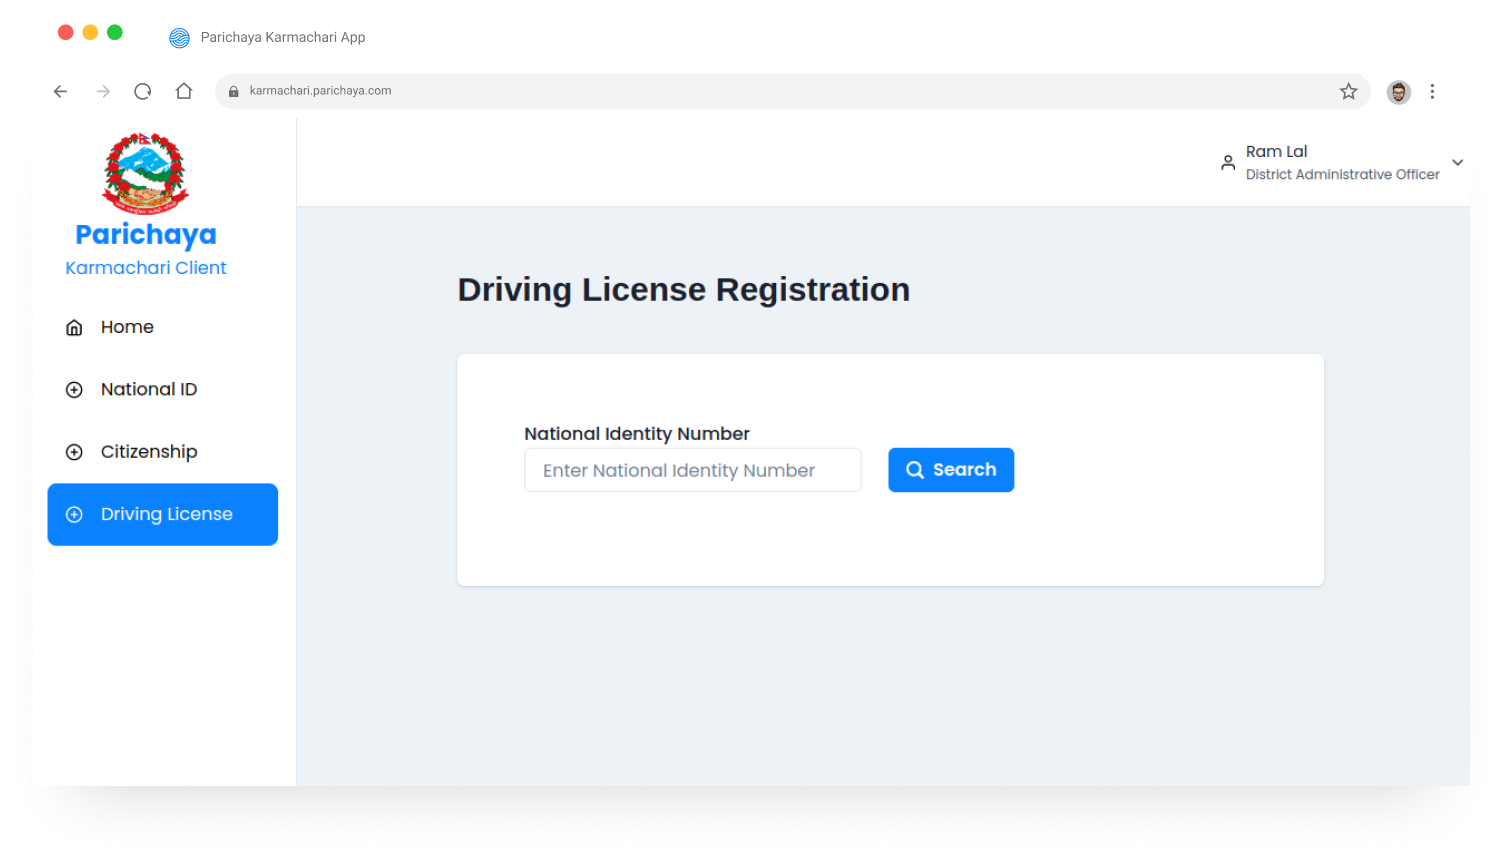
\includegraphics[width=0.8\linewidth]{images/results/web/WebDrivingLiceseRegistration1.png}
        \caption[Enter NIN]{Enter NIN}
        \label{fig:WebDrivingLiceseRegistration1.png}
        \end{figure}
           \begin{figure}[H]
        \centering
        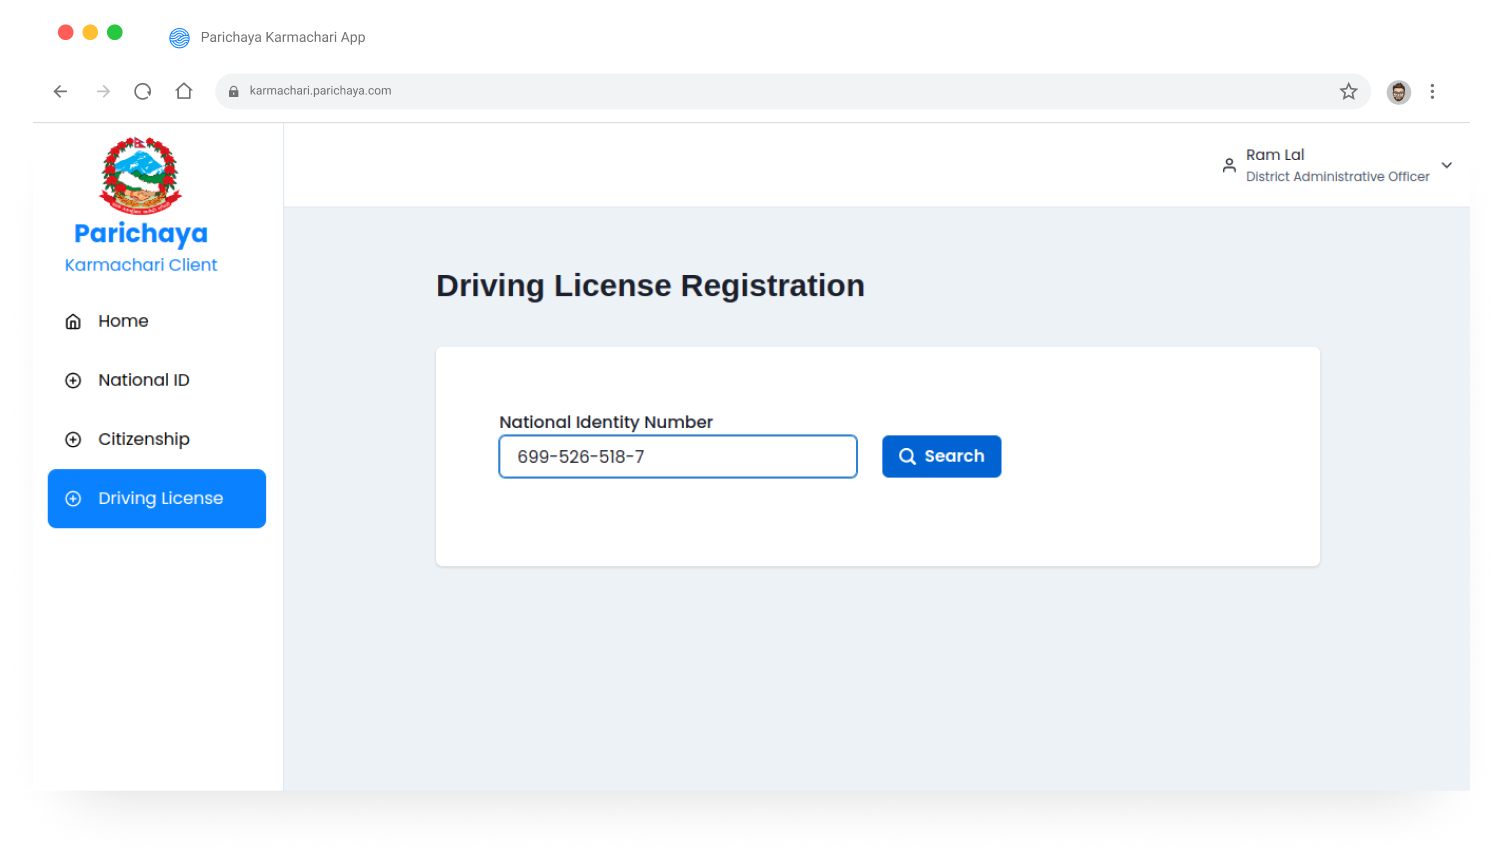
\includegraphics[width=0.8\linewidth]{images/results/web/WebDrivingLicenseRegistration2.png}
        \caption[Driving License Form]{Driving License Form}
        \label{fig:WebDrivingLicenseRegistration2.png}
        \end{figure}


        \begin{figure}[H]
        \centering
        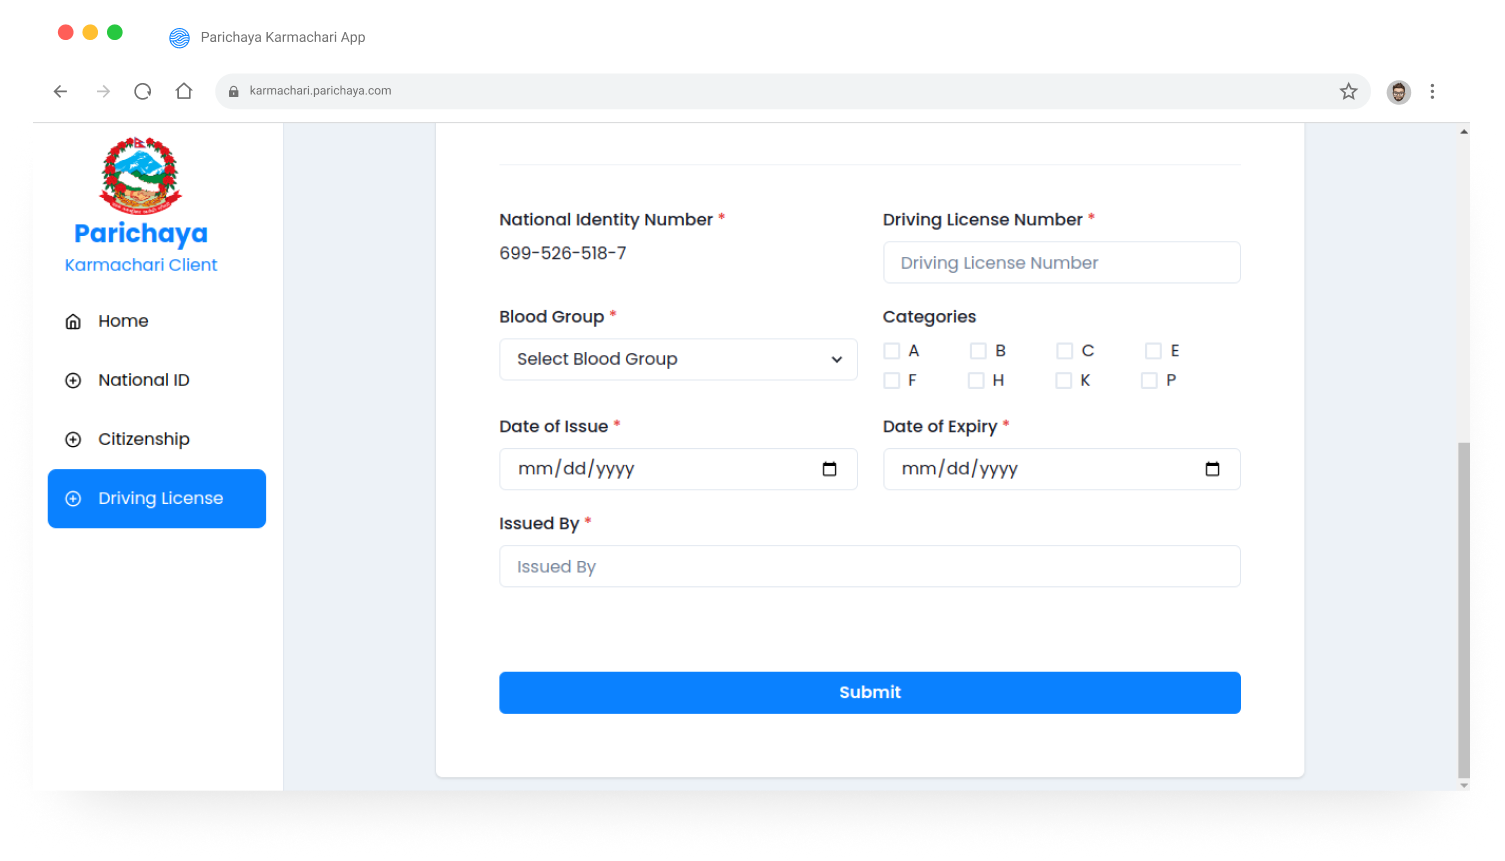
\includegraphics[width=0.8\linewidth]{images/results/web/WebDrivingLicenseRegistration3.png}
        \caption[Driving License Form]{Driving License Form}
        \label{fig:WebDrivingLicenseRegistration3.png}
        \end{figure}
        
    \subsection{Sharing Details to Third Party Web Client}
        User can directly fill form or share identity document details to third party applications like banks or governmental organization through Parichaya with a touch of a button.     
   
        \begin{figure}[H]
        \centering
        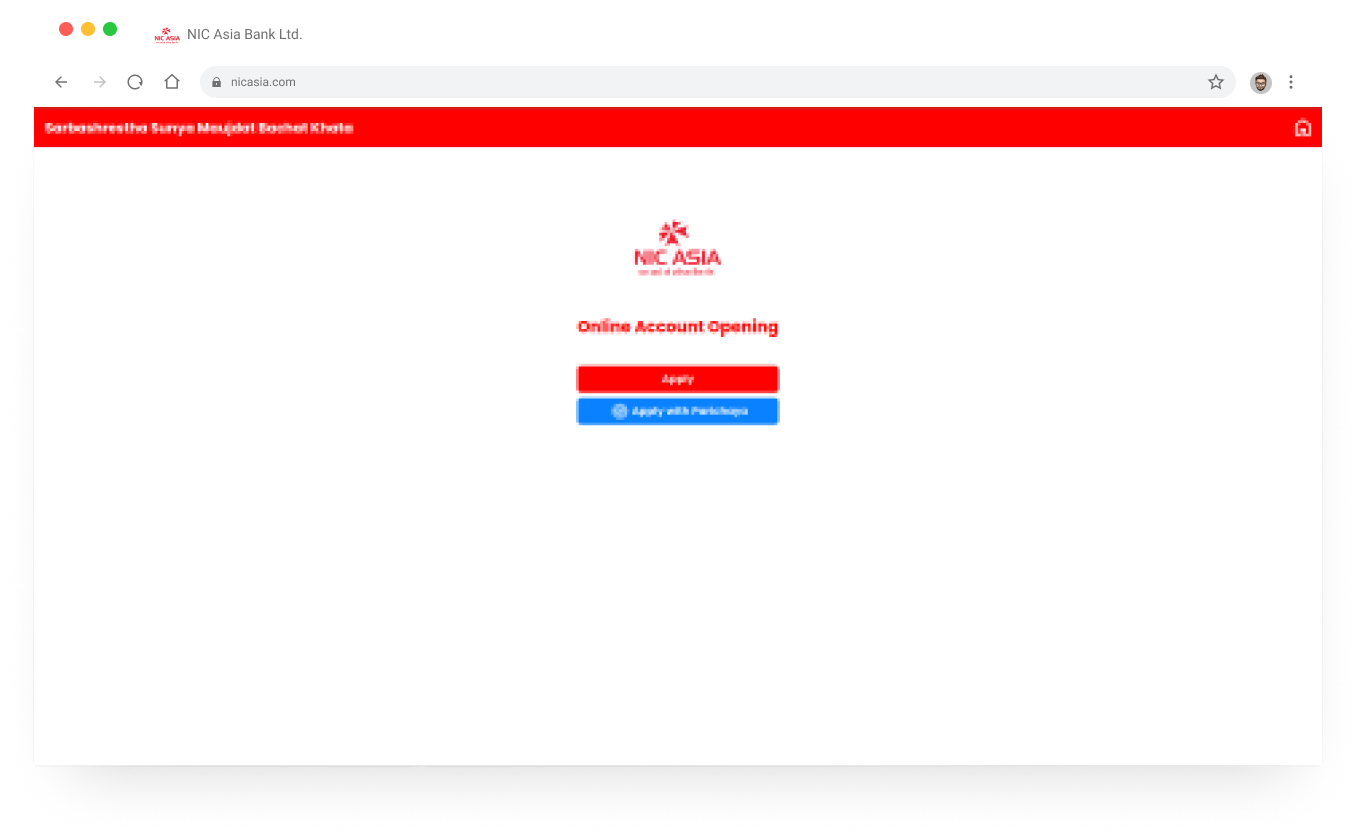
\includegraphics[width=0.8\linewidth]{images/results/web/NICApply.png}
        \caption[Nic Asia Apply]{Nic Asia Apply}
        \label{fig:NICApply.png}
        \end{figure}
        % \newpage
    After clicking the button, a QR code is generated along with the required data fields. Users can scan the QR code using Parichaya mobile app to view the requester's details along with the requested data fields. 
        \begin{figure}[H]
        \centering
        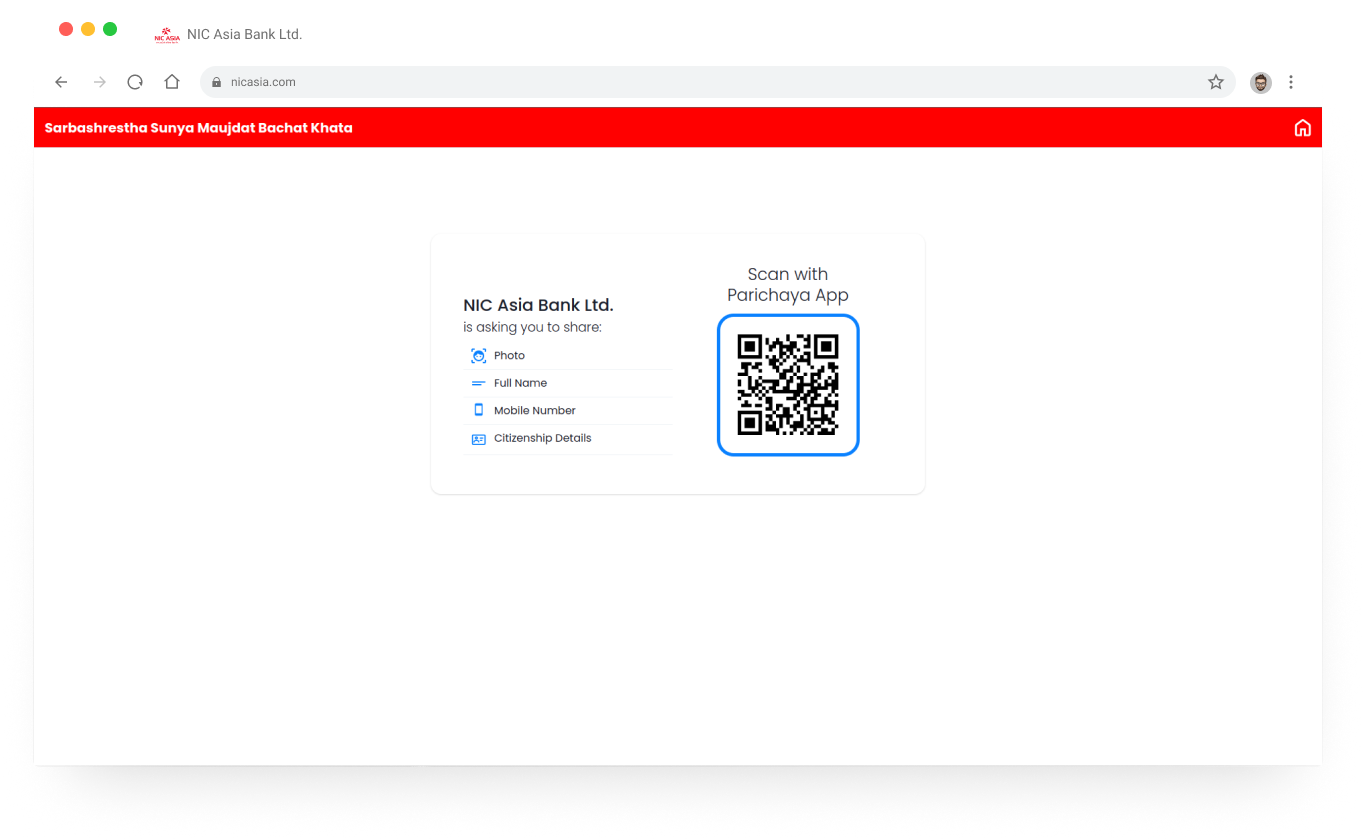
\includegraphics[width=0.8\linewidth]{images/results/web/NICQR.png}
        \caption[Nic Asia QR]{Nic Asia QR}
        \label{fig:NICQR.png}
        \end{figure}
         \begin{figure}[H]
        \centering
        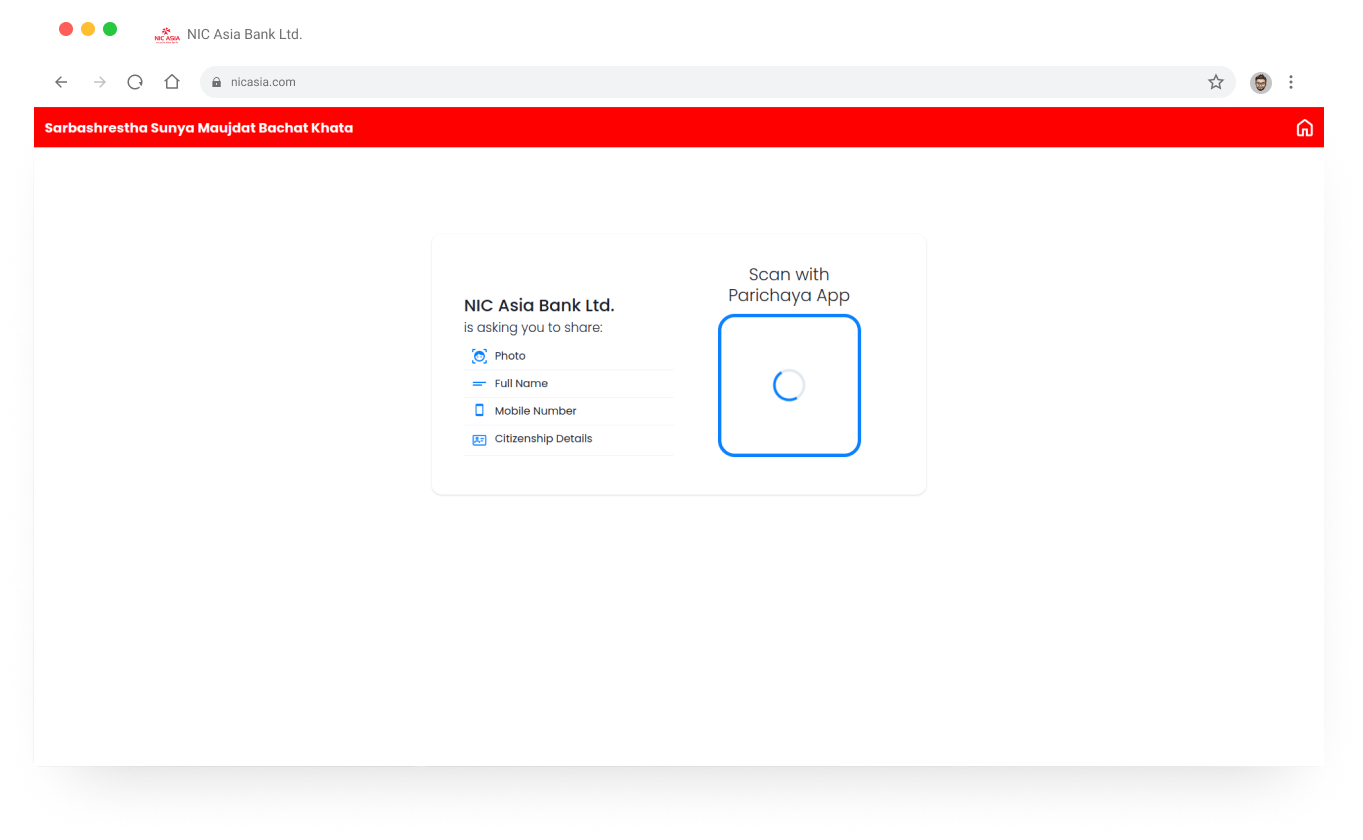
\includegraphics[width=0.8\linewidth]{images/results/web/NICLoading.png}
        \caption[Nic Asia Loading]{Nic Asia Loading}
        \label{fig:NICLoading.png}
        \end{figure}
        % \newpage
        If the user approves the data request, the requested data are shown. Else, a rejection message is showned to the user.  
         \begin{figure}[H]
        \centering
        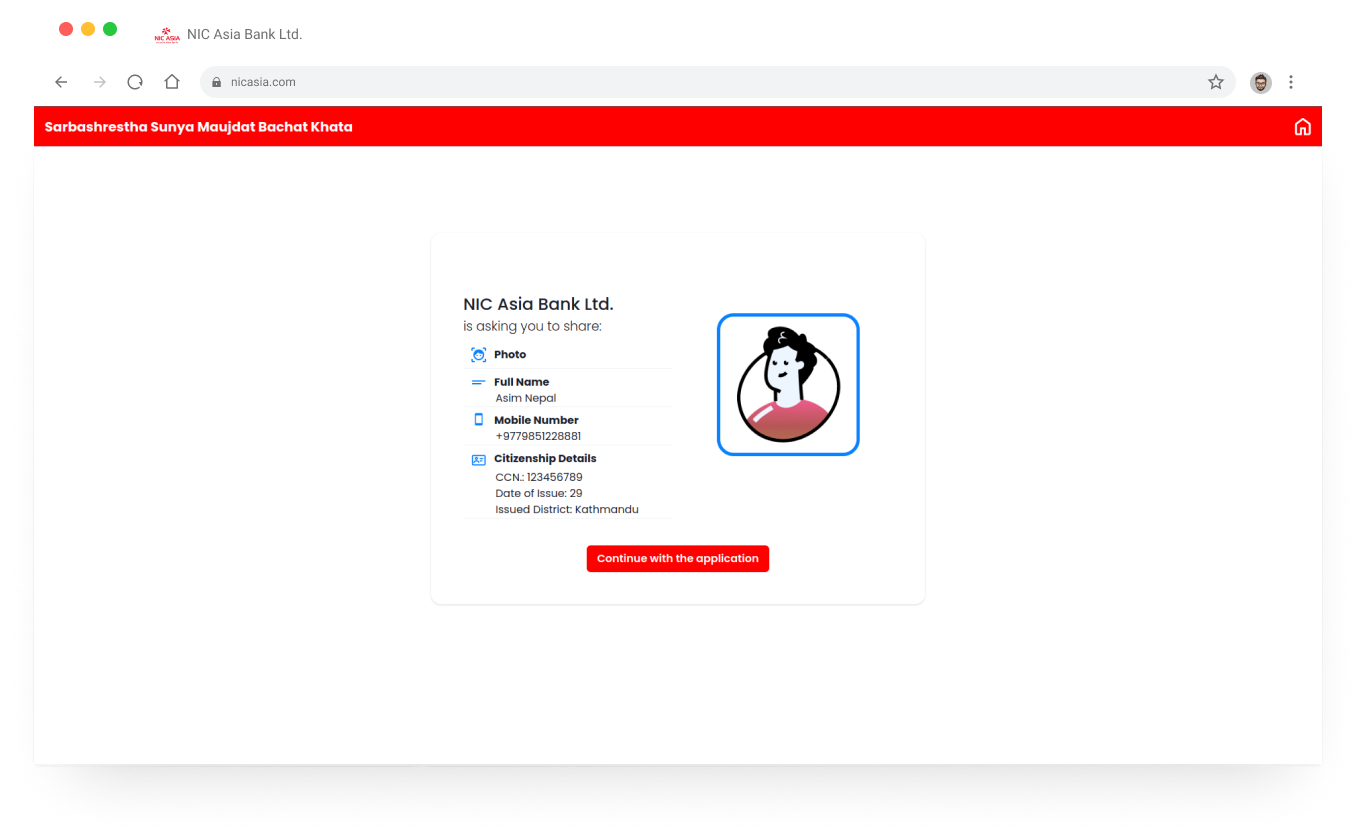
\includegraphics[width=0.8\linewidth]{images/results/web/NICDetails.png}
        \caption[Nic Asia Details]{Nic Asia Details}
        \label{fig:NICDetails.png}
        \end{figure}
        \begin{figure}[H]
        \centering
        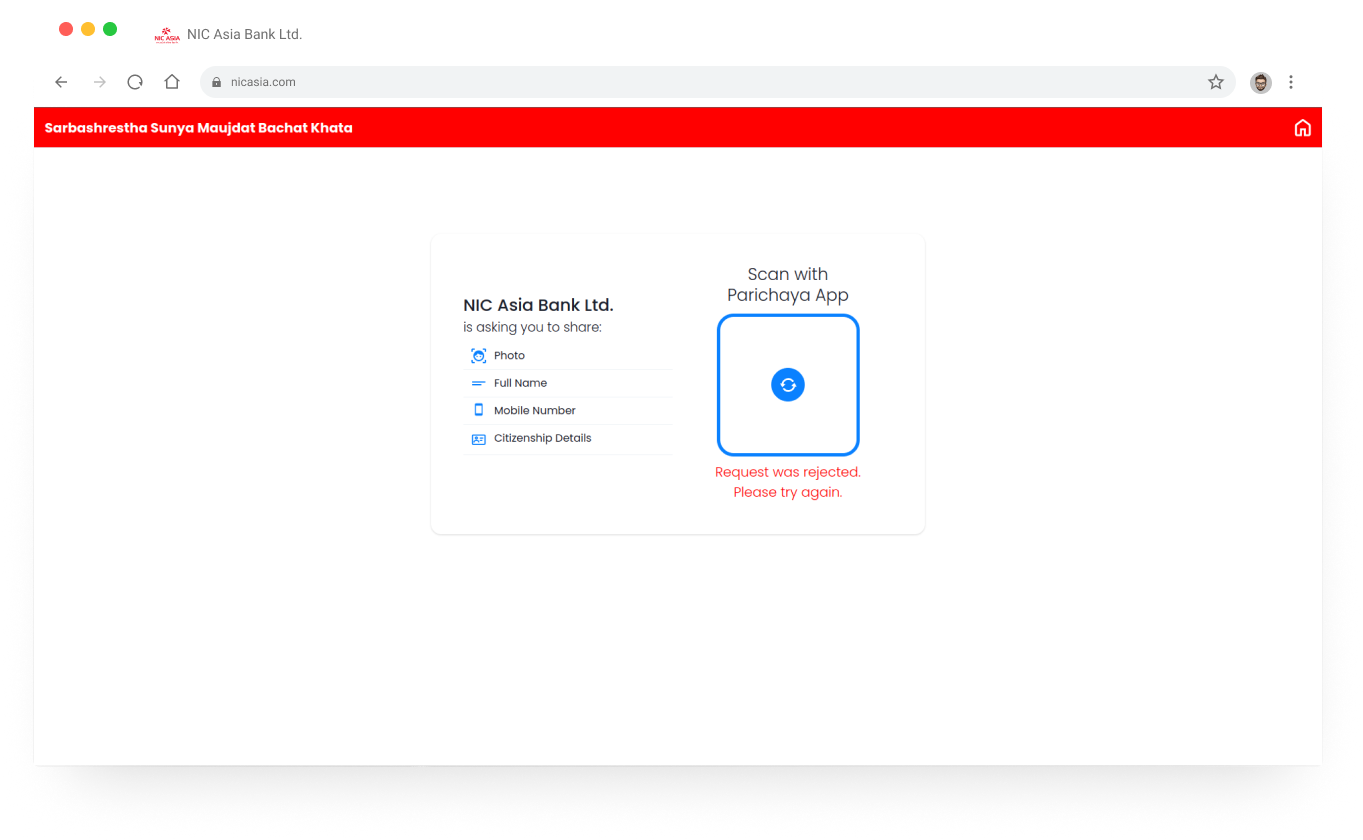
\includegraphics[width=0.8\linewidth]{images/results/web/NICRejected.png}
        \caption[Nic Asia Rejected]{Nic Asia Rejected}
        \label{fig:NICRejected.png}
        \end{figure}
        


\section{Discussion}
The report highlights the need for an upgraded digital authentication system in Nepal, as the current process heavily relies on physical documents and centralized storage, leading to inefficiencies and security risks. To address these challenges, the proposal suggests implementing a blockchain-based digital identity system called "Parichaya" using Hyperledger Fabric technology. The system aims to provide secure and tamper-proof storage of citizens' documents, improve government service delivery, and enhance convenience for users. The use of blockchain technology can prevent identity fraud, ensure data integrity, and enable faster verification processes. While the system presents numerous benefits, there are potential limitations to consider, such as the reliance on government officials' authentication and the need for data encryption to enhance security. However, the proposal also discusses opportunities for future research and application, including integration into other sectors like healthcare, supply chain management, and institutional account creation processes. Overall, the report highlights the importance of upgrading Nepal's authentication system and the potential of blockchain technology to address the identified challenges.

      



% \chapter{DISCUSSION AND ANALYSIS}

% (20\% of Report Length)

% a. Quantitatively presenting output of verification and validation procedures

% b. Comparing between theory and simulation values

% c. Comparing with state-of-the-art work performed by other authors

% d. Performing error analysis and pinpointing possible sources of error

The idea of authenticating a country’s citizen has become a norm for any of the country’s government. Most of the developed countries have developed a well defined system for the online authentication process, which acts as a base for providing government services to the citizens. However, in case of Nepal, the authentication process is well outdated, and in dire need for an upgrade. In our research, we discovered that even the trending applications of Nepal like mobile banking or other wallet applications authenticates it’s user by matching the user’s input
with their physical documents, which must be provided by the user. Furthermore, the government of Nepal, along with other institutions, still requires physical documents for identification and other formal procedures. This might pose as a big problem as it requires time and manpower to verify and maintain the information obtained. Also, the use of physical document has a problem of its own. Neither is it convenient nor is it safe. We might not always have access to the required documents as well. Yet, attempts of digitizing such documents in Nepal just lead to failure. A major cause would be the centralized storage of all the information in one particular place “Singha durbar”, which leads to a single point of failure. The government of Nepal did try to salvage this situation by providing their own mobile application “Nagarik App”, which is performing quite well, though it received a lot of criticism in the earlier stages of development. The app itself relies on the centralized information, so it is prone to single point failure as well.

Through analysis of all the findings from our research, we felt a strong requirement for a better digital ecosystem. One, which is not centralized and prone to single point failure, and is convenient for the Nepali citizens, along with being easy to use for the verification process by government officials, so as to provide governmental services. The base of which is a private and permissioned blockchain technology called “Hyperledger Fabric”. Blockchain technology is a decentralized, digital ledger that is used to record transactions across a network of computers. One of the key features of blockchain technology is that it is secure and tamper-proof, as each block in the chain contains a record of previous transactions and is linked to the previous block through a cryptographic hash. By using a blockchain-based digital identity system, personal information can be stored and verified in a tamper-proof manner, which can help prevent identity fraud and ensure that individuals have control over their personal data. Additionally, blockchain technology can enable faster and more efficient verification of identities for financial transactions, government activities, and other important processes. Overall, a blockchain-based digital identity system can help improve security, efficiency, and transparency of citizens documents in Nepal. 

Hyperledger Fabric can be used for digital identity management by creating a permissioned blockchain network that stores and manages digital identity information. The network would be composed of authorized participants, such as government agencies, financial institutions, and other organizations that need to verify the identity of individuals. This system will solve the problem of authentication regarding digital identification process by simply authenticating the input data itself with the use of blockchain technology. Hyperledger Fabric is used in this project to set up a test network of private blockchain. This test network is simulated in containers using Docker Compose. This test network is configured to contain two organizations, ’Parichaya’ and ’Nepal Government’. Parichaya represents the organization that interacts with the blockchain to provide digital identity services through the Parichaya App. Nepal Government represents the organization that interacts with the blockchain to maintain the digital record of government issued identity documents. The two organizations agree on a channel configuration to jointly collaborate on the channel. The business logic that defines how peer organizations interact with the ledger is contained in a smart contract which is inside a structure called chaincode. This basically has the functions of reading and writing each citizens documents in the blockchain. Primarily, the chaincode transactions are invoked via a client application through the Fabric Gateway Application. This system contains two of such client applications, the Parichaya web app, and the Parichaya mobile app. The web application is connected to the blockchain through the Gateway Application for ‘Nepal Government’, and  can only be used by authenticated government officials, where logs of their activities are also kept for transparency and security purposes. Even corrupted government officials can be kept away from inflicting unwanted modifications in the blockchain. Now, for the problem of physical documents, its replacement can be assured by the use of client mobile application. This app allows users to view their government documents and also allows them to share the details to other users or to some third party application. All of these services are facilitated by the Parichaya backend server, which interacts with the blockchain through the Gateway Application for ‘Parichaya’. This system will ensure safe and secure digitization of Nepal with convenient and easy to use applications.

There have been other researches on this topic which might seem similar to our system in some sense. The research papers or articles with which our system might have certain qualities in common would be “Medusa: Powered Log Storage System”,  “Journal of Network and Computer Applications”, “Blurring the Lines between Blockchains and Database Systems: The Case of Hyperledger Fabric”. Though, most of them are only similar in the use of blockchain and its network and none are trying to solve all of the exact problems that our system does. Whereas there are some applications which are similar for its authentication and storage ability to our mobile application. “Nagarik App” would be the most obvious as our mobile application might seem as an imitation to the government launched application. But, if you look at the whole system itself, the Parichaya mobile application relies on decentralized data and ease of sharing, so it would seem as a major upgrade. Although, Yoti app and Eid-me app, does solve the problem of authentication elegantly, and provides some information details to it’s users, it doesn’t rely on decentralized information, so they both have single point of failure. Furthermore, along with sharing of basic details, the Parichaya app already has some implemented features like sharing verified age as one would need in some cases, along with sharing verified driving license digitally to traffic police. Parichaya app, in fact, also provides better visual graphics of the user’s information than most of the mentioned applications.

Although, this system seems like an answer to digitalizing of Nepal with introduction of digital government documents, it does have some limitations, which can be solved with certain enhancements. Even though, blockchain technology is being used, the citizens data can’t be completely safe. As there are authorities (government officials) who can alter the data. Granted, the log of their actions is kept, and we can find the culprit, but it is only as good as the security of the authentication process of the government officials. If somehow, the authentication of the government officials are compromised, the safety of the citizen’s data cannot be guaranteed. The data stored in the blockchain is not in encrypted form as well, so malicious acts as mentioned before will be easier. There’s also currently only single web application to register users through the government.  But, this can later be modified depending upon the needs of the government. Further, the system only stores three identity documents for the time-being, i.e. Citizenship Card, National Identity Card and Driving License. This can be optimized to digitize other documents to better suit the needs of a citizen. All of the three documents are handled in different government bodies, so it would be a better fit to use individual servers for each of the documents, but in our case, only one server is being used for all types of documents. These are some of the limitations of our system, few of which can cause critical damages.

Considering the future endeavor on avenues of this system for further research based on our findings, there might be a lot of fields where this system might extend through various areas of studies and be used in different contexts. This system has potential to be upgraded into working in sectors other than just governmental works. An implemented example would be filling forms for creating accounts (for institutes like banks or colleges). Any institutes can use the “fill using Parichaya” feature, which generates a QR code for all the required information set by the institutes themselves. The mobile app user can then proceed to  scan the QR code using the Parichaya app scanner. This shows all the information that the user will be sharing, and the user can decide to either approve or deny the request. This feature will surely be handy as the form filling process will be multiple times quicker and the institutes don’t even require to spend time verifying the data. 
Further, the ability to securely store and share identity information can streamline the process of accessing financial services. This can lead to faster processing times, reduced paperwork, and increased accessibility for under-served populations. In case of fields like healthcare, storing patient identities and medical records on a blockchain can improve the efficiency and security of healthcare systems. Medical professionals can quickly and easily verify patient identities, access medical histories, and securely share medical data across different providers. For other government services, this system can streamline the process of accessing government services such as voting, social services, and tax filing. This can increase efficiency, reduce fraud, and improve accountability. As for supply chain management, the ability to securely verify the identity of suppliers and manufacturers on a blockchain can improve transparency and traceability in supply chains. This can help reduce fraud, improve quality control, and enhance consumer confidence. These are few fields in which our system can adapt and improve the current trends of handling data. Our system is naught but a concept for securely, conveniently, and efficiently handling confidential documents of user, and can be used in various fields that require it.

\chapter{CONCLUSION}
\section{CONCLUSION}
% In today's digital age, managing personal data is a complex and challenging task. The amount of personal data that individuals generate and share every day has increased significantly, and the need for a secure and reliable system to store and share personal data has become more critical than ever. With the advent of blockchain technology, there has been a surge in the development of innovative solutions to address this problem. This project is designed to provide a secure and efficient way of storing and sharing personal data using blockchain technology.

% One of the main benefits of using blockchain technology to store personal data is the high level of security it provides. Blockchain technology uses cryptography to secure the data, making it virtually impossible for unauthorized parties to access or tamper with the data. Additionally, the decentralized nature of blockchain technology ensures that there is no single point of failure, making the system highly resistant to attacks.

% The mobile app developed in this project, is designed for convenience of the users. Users can store a personal data, including driving licence information, citizenship information, National Identity Card information. The app ensures that the data is stored securely and is only accessible to the user, ensuring that their privacy is protected at all times. The app contains features which allow users to share their data securely with other institutions, such as banks, to facilitate the process of opening bank accounts, or with other users, such as traffic police or bartenders to verify the users age or driving license. Instead of relying on physical documents that can be lost or stolen, users can share their data securely using the app, making the entirety of the process much more convenient and efficient.

% The project also includes an integration with a government web app developed by the same team. This integration further enhances the security and reliability of the system by enabling users to share their data with government institutions securely. The government web app ensures that the data is transmitted securely, and the use of blockchain technology ensures that the data is tamper-proof.

% In conclusion, this project provides an innovative solution to the problem of managing personal data securely. The use of blockchain technology ensures that the data is stored securely and is only accessible to the user, while the mobile app makes it easy for users to manage and share their data. The integration with government web apps further enhances the security and reliability of the system, making it a comprehensive solution for managing personal data. Overall, this project has the potential to revolutionize the way personal data is managed and shared, making it a valuable asset for individuals and institutions alike.

We've successfully achieved all of the objectives outlined when starting the project. A fully functional Parichaya mobile application and a Karmachari web application has been developed for the use of the citizens and the government officials. Along with the system requirements that had to be implemented, additional features are provided by the application as well. The user interfaces of both the applications have been made simple enough for a layman to use with ease. At the end, the smooth operation of the components in the backend, along with the client applications showed that the system's requirements, designs and implementation were handled correctly. All the deadlines have been met meaning that the schedule chosen was suitable for the project. After completing the project, following results are obtained: 
\begin{itemize}[itemsep=-4pt, topsep=-8pt]
    \item Problem of digital authentication is solved.
    \item The use of physical identity documents is removed.
    \item Decentralization of citizen's document details is achieved. 
\end{itemize}

\section{FUTURE ENHANCEMENTS}

% Enhancements: (1 to 2 Pages)

% a. Mention approaches that were not attempted, but could have been experimented with for better results

% b. Recommended a research path for future researchers that may embark on a similar research topic

\begin{itemize}
    \item Data stored in the blockchain are not encrypted currently. Techniques like threshold cryptography can be added later to the blockchain to make it more secure.
    \item This project only handles three identity documents for the time-being i.e. Citizenship Card, National Identity Card and Driving License. It can be optimized to digitize other documents to better suit the needs of a citizen.
    \item Notifications can be sent to the user when their documents have been updated or modified. 
    
\end{itemize}







% \include{6ProjectSchedule/schedule}

%\newpage

%========================References setup=========================================================
\newpage
\bibliographystyle{ieeetr}
\bibliography{References/references}

\addcontentsline{toc}{chapter}{REFERENCES}

%=============================================================================================

% ================================Appendices Setup================================================

% \appendix
% \chapter{Docker}
% \section{Appendix A.1}        % Do not show in table of content.
% \subsection{Appendix A.1.1}   % Do not show in table of content.
% \chapter{Appendix B}
% \section{Appendix B.1}        % Do not show in table of content.
% \section{Appendix B.2}  

\begin{appendices}

% \addtocontents{toc}{\textbf{APPENDICES}}

\chapter*{APPENDICES}
\addcontentsline{toc}{chapter}{APPENDICES}

% \renewcommand\thefigure{\thechapter.\arabic{figure}}
\newcommand{\nocontentsline}[3]{}
\newcommand{\tocless}[2]{\bgroup\let\addcontentsline=\nocontentsline#1{#2}\egroup}

\renewcommand\thesection{\Alph{section}}
\renewcommand\thesubsection{\thesection.\arabic{subsection}}


\titleformat{\section}{
\normalfont\fontsize{12}{15}\bfseries
}{APPENDIX \thesection:}{1em}{}


\titlespacing{\section}{0pt}{-0.5in}{0.5em}

\renewcommand\thefigure{\thesection.\arabic{figure}}


\section{Project Schedule}
\vspace{10pt}


\includegraphics[width=1 \linewidth]{images/appendix/Gantt.png}



\captionof{figure}[Gantt Chart Showing Expected Project Timeline]{
Gantt Chart Showing Expected Project Timeline
}

 \newpage




\section{Containerization of Blockchain and Backend Servers}
\vspace{10pt}
\includegraphics[width=1 \linewidth]{images/appendix/Docker.png}

\setcounter{figure}{0}  

\captionof{figure}[Blockchain Nodes and Backend Servers Running in Docker Containers]{
Blockchain Nodes and Backend Servers Running in Docker Containers
}

 \newpage




\section{Project Setup Guide}
\vspace{15pt}

\tocless\subsection{Setup Guide to run Blockchain and Gateway Application}
\vspace{15pt}
\textbf{Prerequisite:}

\begin{itemize}[noitemsep]
    \item Linux OS
    \item Docker compose
    \item Jq
    \item Git
    \item cURL
    \item Docker
    \item JQ
    \item Node (version 18 and above)
\end{itemize}

\textbf{Clone the repo from github.}
\begin{verbatim}
    git clone git@github.com:nepal80m/pochita.git
\end{verbatim}

\textbf{Install the required binaries and configurations for the blockchain network.}
\begin{verbatim}
    curl -sSLO
    https://raw.githubusercontent.com/hyperledger/fabric/main/
        scripts/install-fabric.sh 
    chmod +x install-fabric.sh 
    ./install-fabric.sh d b
    rm install-fabric.sh
\end{verbatim}
\textbf{Command to Install the required packages for rest api server:}
\begin{verbatim}
    cd restapi/
    npm install
    cd ..
\end{verbatim}

\textbf{Command to start the blockchain network:}
\begin{verbatim}
    cd scripts/
    ./wakeup.sh
    cd ..
\end{verbatim}

\textbf{Command to run the rest api server:}
\begin{verbatim}
    cd restapi/
    npm run dev
    cd .. 
\end{verbatim}


\tocless\subsection{Setup Guide to run Parichaya Backend Server} 
\vspace{15pt}
\textbf{Clone the repo from github.}
\begin{verbatim}
    git clone git@github.com:nepal80m/dr-octavius.git
\end{verbatim}
\textbf{To start the docker container, run the following command.}
\begin{verbatim}
    docker compose up
\end{verbatim}

\tocless\subsection{Setup Guide to run Parichaya App} 
\vspace{15pt}
\textbf{Clone the repo from github.}
\begin{verbatim}
    git clone git@github.com:Nischal-Shakya/project-vegapunk.git
\end{verbatim}

\textbf{Command to get all the dependencies:}
\begin{verbatim}
    flutter pub get
\end{verbatim}

\textbf{Command to build the flutter app in the connected device:}
\begin{verbatim}
    flutter run
\end{verbatim}

 \newpage




% \input{Appendix/appendix4.tex}
\end{appendices}







%=========================================================================
\end{document}